\chapter{Signed kernels and certified polylogarithm computation}
\label{ch:certified-computation}
The exact reductions suggest evaluation methods that expose more analytic
structure. A signed density for $F_{a,b}(z)=\Li_{a,b}(z,1)$ proves a unique
angular zero and makes Gaussian Euler errors one-sided. The general double
integral supports Chebyshev and midpoint expansions, while Holder convolution
provides uniform rational certificates for a wider alphabet. These methods
connect experiments, geometry and finite arithmetic: their tail theorems and
rounding contracts determine what a numerical comparison establishes.
Write $D_{a,b}(x,y)=\Li_{a,b}(x,y)$. Throughout the signed-density discussion,
$H_n^{(b)}=\sum_{j=1}^n j^{-b}$, $H_0^{(b)}=0$, and
$g_{a,b}=\Imag F_{a,b}(\iu)$; real $b>0$ is allowed where stated.

\section{A signed-kernel representation}
\label{signed:sec:kernel}

\begin{definition}\label{signed:def:kappa}
For real $b>0$ and $T>0$, define
\begin{equation}\label{signed:eq:kappa-base}
 \kappa_{1,b}(e^{-T})=
 -\frac{T^b}{\Gamma(b+1)}
 +\frac1{\Gamma(b)}\int_T^\infty\frac{v^{b-1}}{e^v-1}\dd v.
\end{equation}
For an integer $a\ge2$, define successively
\begin{equation}\label{signed:eq:kappa-recursion}
 \kappa_{a,b}(u)=\int_u^1\frac{\kappa_{a-1,b}(v)}{v}\dd v,
 \qquad 0<u<1.
\end{equation}
\end{definition}

\begin{theorem}[Moments and one sign change]\label{signed:thm:kernel}
For every integer $a\ge1$ and real $b>0$, the density $\kappa_{a,b}$ is integrable on $(0,1)$ and
\begin{equation}\label{signed:eq:kernel-moments}
 \int_0^1u^{n-1}\kappa_{a,b}(u)\dd u
 =\frac{H_{n-1}^{(b)}}{n^a},\qquad n\ge1.
\end{equation}
In particular its total mass is zero. There is exactly one $r_{a,b}\in(0,1)$ such that
\begin{equation}\label{signed:eq:kernel-sign}
 \kappa_{a,b}(u)<0\quad(0<u<r_{a,b}),\qquad
 \kappa_{a,b}(u)>0\quad(r_{a,b}<u<1).
\end{equation}
The crossing is strict, and $r_{a,b}<r_{a-1,b}$ when $a\ge2$.
\end{theorem}
\begin{proof}
First consider $a=1$. The negative term in \eqref{signed:eq:kappa-base} has moment $-n^{-b-1}$. Substituting $u=e^{-T}$ and interchanging nonnegative integrands in the positive term gives
\begin{align*}
 &\frac1{\Gamma(b)}\int_0^\infty e^{-nT}
       \int_T^\infty\frac{v^{b-1}}{e^v-1}\dd v\dd T\\
 &\hspace{12mm}=\frac1{n\Gamma(b)}\int_0^\infty
       \frac{v^{b-1}(1-e^{-nv})}{e^v-1}\dd v
 =\frac1n\sum_{k=1}^n k^{-b}.
\end{align*}
The final equality uses the finite geometric identity
$(1-e^{-nv})/(e^v-1)=\sum_{k=1}^n e^{-kv}$.
Subtracting $n^{-b-1}$ proves the base moment formula. At $n=1$, both positive and negative terms have finite integral~1, so integrability and zero mass are established without subtracting divergent quantities.

As a function of $T$, the base density has derivative
\begin{equation}\label{signed:eq:kappa-base-derivative}
 \frac{\mathrm d}{\mathrm dT}\kappa_{1,b}(e^{-T})
 =-\frac{T^{b-1}}{\Gamma(b)(1-e^{-T})}<0.
\end{equation}
It is positive as $T\downarrow0$: the limit is $\zeta(b)>0$ if $b>1$, and is $+\infty$ if $0<b\le1$. It tends to $-\infty$ as $T\to\infty$. Thus it has exactly one crossing, with the sign pattern stated in the $u$ coordinate.

For the induction, the integral operator in \eqref{signed:eq:kappa-recursion} is an $L^1$ contraction:
\[
 \int_0^1\left|\int_u^1\frac{f(v)}v\dd v\right|\dd u
 \le\int_0^1|f(v)|\dd v.
\]
Fubini's theorem gives the moment of the new density as $1/n$ times the previous moment; in particular it preserves zero mass. If the preceding crossing is $r$, the new density is positive on $[r,1)$, while on $(0,r)$ its derivative is $-\kappa_{a-1,b}(u)/u>0$. Zero mass forces it to be negative somewhere on that interval. Strict increase then gives exactly one crossing in $(0,r)$. This completes the induction.
\end{proof}

\begin{corollary}[Integral continuation]\label{signed:cor:stieltjes}
For $z\in\mathbb C\setminus[1,\infty)$,
\begin{equation}\label{signed:eq:stieltjes}
 F_{a,b}(z)=\int_0^1\frac{z}{1-zu}\kappa_{a,b}(u)\dd u.
\end{equation}
In particular, if $0<\theta<\pi$,
\begin{equation}\label{signed:eq:angular-integral}
 \Imag F_{a,b}(e^{\iu\theta})
 =\sin\theta\,J_{a,b}(\cos\theta),\qquad
 J_{a,b}(c)=\int_0^1\frac{\kappa_{a,b}(u)}{1-2cu+u^2}\dd u.
\end{equation}
\end{corollary}
\begin{proof}
For $|z|<1$, expand $z/(1-zu)$ and use the moments. On compact subsets of the slit plane the denominator is bounded away from zero uniformly in $u\in[0,1]$, so the integral is analytic there. This continues the disk identity. Taking the imaginary part of $e^{\iu\theta}/(1-ue^{\iu\theta})$ gives \eqref{signed:eq:angular-integral}.
\end{proof}

\begin{lemma}[A sign test for zero-mass densities]\label{signed:lem:sign-test}
Let $\kappa$ have zero integral and the strict sign pattern \eqref{signed:eq:kernel-sign}, with crossing $r$. If $q$ is strictly decreasing and the integral exists, then $\int q\kappa<0$. If $q$ is strictly increasing, the sign is positive.
\end{lemma}
\begin{proof}
Subtract $q(r)\int\kappa=0$. The product $(q(u)-q(r))\kappa(u)$ has the asserted strict sign on each side of $r$.
\end{proof}

\section{The unique zero on the upper semicircle}
\label{signed:sec:zeros}

\begin{theorem}[Existence, uniqueness, and simplicity]\label{signed:thm:unique-zero}
Let $a\ge1$ be an integer and let $b>0$ be real. There is exactly one
$\theta_{a,b}\in(0,\pi)$ such that
$\Imag F_{a,b}(e^{\iu\theta_{a,b}})=0$. It satisfies
\begin{equation}\label{signed:eq:zero-range}
 0<\theta_{a,b}<\frac\pi2.
\end{equation}
The imaginary part is positive for $0<\theta<\theta_{a,b}$ and negative for $\theta_{a,b}<\theta<\pi$. At its zero the angular derivative is strictly negative. Consequently,
\begin{equation}\label{signed:eq:g-negative}
 g_{a,b}<0.
\end{equation}
\end{theorem}
\begin{proof}
Suppress the indices in $J$ and $\kappa$. The kernel $u\mapsto(1+u^2)^{-1}$ is strictly decreasing, so Lemma~\ref{signed:lem:sign-test} gives $J(0)<0$.

We next show that the limit of $J(c)$ as $c\uparrow1$ is positive, possibly infinite. The negative density is supported in $(0,r)$, away from the singular endpoint, and its contribution has a finite limit. On $(r,1)$ monotone convergence applies. Expanding $(1-u)^{-2}$, treating these two parts separately, and using \eqref{signed:eq:kernel-moments} yields
\begin{equation}\label{signed:eq:J-at-one}
 \lim_{c\uparrow1}J(c)
 =\int_0^1\frac{\kappa(u)}{(1-u)^2}\dd u
 =\sum_{n\ge0}\frac{H_n^{(b)}}{(n+1)^{a-1}}>0.
\end{equation}
Every summand from $n=1$ onward is positive. Thus continuity produces at least one zero $c_0\in(0,1)$.

For uniqueness, write $K_c(u)=(1-2cu+u^2)^{-1}$. If $c'>c$, then
\begin{equation}\label{signed:eq:kernel-ratio}
 \frac{\mathrm d}{\mathrm du}\frac{K_{c'}(u)}{K_c(u)}
 =\frac{2(c'-c)(1-u^2)}{(1-2c'u+u^2)^2}>0.
\end{equation}
At a zero $J(c)=0$, the signed density $K_c\kappa$ still has one sign change and zero mass. Applying Lemma~\ref{signed:lem:sign-test} to the ratio in \eqref{signed:eq:kernel-ratio} gives $J(c')>0$ for every $c'>c$. The same argument with a smaller parameter gives $J(c')<0$ for $c'<c$. There can be only one zero in $(-1,1)$, with the indicated signs.

Finally,
\[
 J'(c_0)=\int_0^1 K_{c_0}(u)\kappa(u)
        \frac{2u}{1-2c_0u+u^2}\dd u>0,
\]
because the last factor has derivative $2(1-u^2)/(1-2c_0u+u^2)^2>0$. Equation~\eqref{signed:eq:angular-integral} therefore has derivative
$-\sin^2\theta_{a,b}\,J'(c_0)<0$ at $\theta_{a,b}=\arccos c_0$. Since $c_0>0$, this zero is below $\pi/2$. The Gaussian inequality is its value at $\theta=\pi/2$.
\end{proof}

\begin{remark}[The first zero is elementary]
The identity $F_{1,1}(z)=\tfrac12\log^2(1-z)$ gives
\[
 \Imag F_{1,1}(e^{\iu\theta})
 =\log\!\left(2\sin\frac\theta2\right)\frac{\theta-\pi}{2}.
\]
Hence $\theta_{1,1}=\pi/3$ and $g_{1,1}=-\pi\log2/8$. This example also checks the direction of the sign change in Theorem~\ref{signed:thm:unique-zero}.
\end{remark}

\section{A four-term asymptotic for the zero}
\label{signed:sec:zero-asymptotic}
Put $\delta_{a,b}=\pi/2-\theta_{a,b}$. The first surviving Fourier mode at $\pi/2$ is the $n=3$ term, whereas the $n=2$ term controls the derivative. Their ratio suggests $(2/3)^a$; the theorem below identifies both the next Fourier corrections and the first nonlinear correction.

\begin{theorem}[Uniform zero asymptotic]\label{signed:thm:zero-asymptotic}
For integer $a\to\infty$, uniformly for real $b\ge1$, set
$A=H_2^{(b)}$, $B=H_3^{(b)}$, and $C=H_4^{(b)}$. Then
\begin{align}\label{signed:eq:zero-asymptotic}
 \delta_{a,b}
 &=\frac A2\left(\frac23\right)^a
   -\frac C2\left(\frac25\right)^a
   +AB\left(\frac13\right)^a
   -\frac{23A^3}{48}\left(\frac8{27}\right)^a
   +O\!\left(\left(\frac27\right)^a\right).
\end{align}
The implied constant and the threshold for $a$ can be chosen independently of $b\ge1$.
\end{theorem}
\begin{proof}
For sufficiently large $a$, the boundary series and its derivative converge absolutely. Normalize the imaginary part by multiplying by $2^a$, and write $\theta=\pi/2-\delta$. The modes $n=2,3,4,5$ give
\begin{align}\label{signed:eq:zero-fourier}
 0={}&\sin(2\delta)-Aq^a\cos(3\delta)-Bs^a\sin(4\delta)
       +Cr^a\cos(5\delta)\notag\\
    &\quad+O\!\left(\delta\,3^{-a}+(2/7)^a\right),
 \qquad q=\frac23,\quad s=\frac12,\quad r=\frac25.
\end{align}
The $n=6$ mode is $O(\delta3^{-a})$. For $n\ge7$, the bound
$H_{n-1}^{(b)}\le1+\log n$ gives a uniform tail estimate: for $a\ge3$,
\[
 \sum_{n\ge7}(1+\log n)(2/n)^a
 \le (2/7)^a\sum_{n\ge7}(1+\log n)(7/n)^3.
\]
The constant is finite and independent of $b$.

Since $1\le A\le3/2$ and $B,C$ are bounded uniformly in $b$, the normalized expression is negative at $\delta=0$ and positive at $\delta=q^a$ for all sufficiently large $a$. Theorem~\ref{signed:thm:unique-zero} identifies the root in that interval. Thus $\delta=O(q^a)$ uniformly.

Taylor expansion of \eqref{signed:eq:zero-fourier} now gives
\begin{align}\label{signed:eq:zero-expanded}
 0={}&2\delta-Aq^a-4Bs^a\delta+Cr^a
       +\frac92Aq^a\delta^2-\frac43\delta^3
       +O((2/7)^a).
\end{align}
For example, the omitted terms have exponential bases bounded by
$q^5$, $sq^3$, $rq^2$, and $q/3$, all smaller than $2/7$. Insert first
$\delta_0=Aq^a/2$. The linear perturbation $-4Bs^a\delta_0$ requires the correction $AB(qs)^a$, while the $n=5$ mode requires $-Cr^a/2$.
The cubic contribution at $\delta_0$ is
\[
 \frac92Aq^a\delta_0^2-\frac43\delta_0^3
 =\frac{23}{24}A^3q^{3a},
\]
so its compensating correction is $-23A^3q^{3a}/48$.
Substitution of the full displayed approximation in \eqref{signed:eq:zero-expanded} leaves a residual $O((2/7)^a)$; all cross-products of the corrections have smaller exponential bases. The derivative of the normalized expression with respect to $\delta$ is $2+o(1)$, uniformly on this interval. The mean-value theorem therefore converts the residual estimate into the error in \eqref{signed:eq:zero-asymptotic}.
\end{proof}

\begin{center}
\small
\begin{tabular}{@{}rrrr@{}}
\toprule
$a$ & $b$ & $\theta_{a,b}$, approximately & $\delta_{a,b}$, approximately\\
\midrule
8&1&1.541868140889&0.02892818590626\\
8&2&1.546656477391&0.02413984940401\\
8&4&1.550268639150&0.02052768764464\\
12&1&1.565028587360&0.005767739435093\\
12&2&1.565988233290&0.004808093504888\\
12&4&1.566708834682&0.004087492112621\\
20&1&1.570570790993&0.0002255358018452\\
20&2&1.570608378737&0.0001879480579893\\
20&4&1.570636570306&0.0001597564888279\\
\bottomrule
\end{tabular}
\end{center}
These entries are numerical illustrations from a 300-term Fourier sum, not certified root intervals. Existence, uniqueness, and the asymptotic estimate do not depend on the table. At $a=20,40,80$ and $b=1,2,8$, the computed next normalized remainder approaches $H_6^{(b)}/2$, as suggested by the $n=7$ mode. A systematic expansion beyond the proved four terms is a separate research problem.

\section{Certified Euler evaluation}
\label{signed:sec:euler}

\subsection{A one-sided rational enclosure}
Define the difference operator with the sign convention
\[
 (Df)(n)=f(n)-f(n+1).
\]
This is the negative of the usual forward difference; it makes the Euler transformation particularly simple. Let
\begin{equation}\label{signed:eq:euler-data}
 f_{a,b}(n)=\frac{H_{2n}^{(b)}}{(2n+1)^a},\qquad
 d_k=D^kf_{a,b}(0),\qquad
 E_N(a,b)=\sum_{k=0}^{N-1}\frac{d_k}{2^{k+1}}.
\end{equation}

\begin{theorem}[Signed Euler certificate]\label{signed:thm:euler-certificate}
For positive integers $a,b$,
\begin{equation}\label{signed:eq:euler-signs}
 d_0=0,\qquad d_k<0\quad(k\ge1),\qquad
 g_{a,b}=\sum_{k\ge0}\frac{d_k}{2^{k+1}}.
\end{equation}
For every $N\ge1$,
\begin{equation}\label{signed:eq:euler-enclosure}
 E_N(a,b)-C_b2^{-N}\le g_{a,b}\le E_N(a,b),\qquad
 C_b=\begin{cases}1,&b=1,\\ b/(b-1),&b\ge2.\end{cases}
\end{equation}
The approximants decrease strictly from $E_1=0$ to $g_{a,b}$.
\end{theorem}
\begin{proof}
The moment representation gives
\begin{equation}\label{signed:eq:d-kernel}
 d_k=\int_0^1(1-u^2)^k\kappa_{a,b}(u)\dd u.
\end{equation}
For $k=0$ this is zero mass. For $k\ge1$ the weight is strictly decreasing, so Lemma~\ref{signed:lem:sign-test} gives $d_k<0$.

We bound either signed mass of the density. When $b=1$,
\[
 \kappa_{1,1}(u)=\log\frac{u}{1-u},\qquad
 \int_0^1(\kappa_{1,1})_+\dd u=\log2<1.
\]
When $b\ge2$, the positive term of \eqref{signed:eq:kappa-base} is at most $\zeta(b)$, so the positive mass is at most $\zeta(b)<1+1/(b-1)=C_b$. Zero mass makes the negative mass equal to the positive mass. The $L^1$ contraction used in Theorem~\ref{signed:thm:kernel}, together with preservation of zero mass, gives the same bound for every $a$. Since $0\le(1-u^2)^k\le1$, we obtain $|d_k|\le C_b$.

The series in \eqref{signed:eq:euler-signs} is now absolutely convergent. Summing its geometric kernel gives
\[
 \sum_{k\ge0}\frac{d_k}{2^{k+1}}
 =\int_0^1\frac{\kappa_{a,b}(u)}{1+u^2}\dd u
 =g_{a,b},
\]
where the last equality is \eqref{signed:eq:stieltjes} at $z=\iu$. All tail terms are negative, and their total absolute value is at most $C_b\sum_{k\ge N}2^{-k-1}=C_b2^{-N}$. This proves the certificate and strict monotonicity.
\end{proof}

The theorem is stronger than applying a general-purpose extrapolation rule and observing stability. Every endpoint in \eqref{signed:eq:euler-enclosure} is rational. For $N=400$, the interval width is at most $2\cdot2^{-400}<8\cdot10^{-121}$. The accompanying files round the enclosures outward to convenient decimal strings; that display rounding is separate from the internal rational width.

\subsection{An exact linear-work finite formula}
Computing a full triangular difference table uses quadratic work. A finite rearrangement avoids it.

\begin{proposition}[Binomial-tail weights]\label{signed:prop:euler-weights}
For $N\ge1$,
\begin{equation}\label{signed:eq:euler-weighted}
 E_N(a,b)=2^{-N}\sum_{n=0}^{N-1}(-1)^n
 \frac{H_{2n}^{(b)}}{(2n+1)^a}\sum_{j=n+1}^{N}\binom Nj.
\end{equation}
At fixed $a,b$, the right side can be formed with $O(N)$ exact rational or integer updates after choosing $N$. All denominators divide
\begin{equation}\label{signed:eq:denominator-bound}
 2^N\operatorname{lcm}(1,2,\ldots,2N)^{a+b}.
\end{equation}
In particular, the number of bit operations is polynomial in the requested precision at fixed indices.
\end{proposition}
\begin{proof}
Expand $D^kf(0)=\sum_{n=0}^k(-1)^n\binom kn f(n)$ and interchange the two finite sums. The required weight identity is
\[
 \sum_{k=n}^{N-1}2^{N-k-1}\binom kn
 =\sum_{j=n+1}^N\binom Nj.
\]
It follows by induction on $N$ using Pascal's recurrence, or by comparing binomial-tail generating functions. This proves \eqref{signed:eq:euler-weighted}.

The binomial coefficients are generated successively by
$\binom Nn=\binom N{n-1}(N-n+1)/n$, and the cumulative tail is updated by subtracting one coefficient. Each harmonic number is updated by two rational summands. Thus only linearly many updates are needed. Each summand's denominator divides the indicated least-common-multiple power, and the additional factor is $2^N$.
Finally, the elementary bound $\operatorname{lcm}(1,\ldots,2N)\le(2N)!$ gives bit length $O(N+(a+b)N\log N)$ for a common denominator; the numerator has a comparable polynomial bound. Since $N=O(d)$ suffices for $d$ decimal places by \eqref{signed:eq:euler-enclosure}, even elementary integer arithmetic proves polynomial bit complexity. No optimal multiplication or sharp least-common-multiple estimate is required.
\end{proof}

\subsection{Independent depth-one interval arithmetic}
The right sides of the reductions are evaluated using rational enclosures separate from the Gaussian evaluator. For $s\ge1$, the sequences $(2n+1)^{-s}$ and $(n+1)^{-s}$ are moments of positive densities, so all their $D$-differences are nonnegative. Their Euler sums give lower bounds for $\beta(s)$ and $\eta(s)$, with tails at most $2^{-N}$. For integer $s\ge2$, divide the latter interval by $1-2^{1-s}$ to enclose $\zeta(s)$.

For $\pi$, the implementation uses Machin's formula
\[
 \pi=16\arctan(1/5)-4\arctan(1/239)
\]
and the alternating-series bounds for each rational arctangent series. The identity follows directly by tangent addition and the fact that the angle lies in the first quadrant. For $\log2$, it uses
\begin{equation}\label{signed:eq:log2-bound}
 0<\log2-2\sum_{n=0}^{N-1}\frac1{(2n+1)3^{2n+1}}
 \le\frac9{4(2N+1)3^{2N+1}}.
\end{equation}
The expansion is $2\operatorname{arctanh}(1/3)$; the bound replaces the remaining denominators by $2N+1$ and sums a geometric series.

Ordinary rational interval addition and multiplication then enclose every polynomial right side. An overlap check can detect an erroneous formula or implementation if the intervals separate. Overlap alone does not prove an identity; the proofs in Sections~\ref{gaussian:sec:double-parity} and~\ref{gaussian:sec:shuffle} do that.

\subsection{Affine harmonic sequences as signed moments}
\label{affine:sec:moments}
The signed-measure formulation also certifies sequences whose harmonic and
denominator steps differ. The Cayley continuation supplies the integer-order
case; its Gamma-density argument extends without change to real outer order
$a\ge1$. It complements the sharper one-sided bounds above.

\begin{theorem}[Affine signed-moment bound]\label{affine:thm:moments}
Let $r,d$ be positive integers, $a\ge1$ real and $b>0$ real. Set
\[
 A_k=\frac{H_{rk}^{(b)}}{(dk+1)^a},\qquad
 m_1=1,\qquad m_a=\frac{(a-1)^{a-1}e^{-(a-1)}}{\Gamma(a)}\quad(a>1).
\]
There is a finite signed measure $\nu$ on $[0,1]$, with no atom at one,
such that $A_k=\int x^k\,d\nu(x)$ and
\[
 \|\nu\|_{\rm TV}\le\frac{2r}{d}m_a b\zeta(b+1).
\]
For $b>1$ one also has $\|\nu\|_{\rm TV}\le2\zeta(b)$.
Consequently the ordinary alternating series converges, and its $N$-term
Euler transform $E_N$ satisfies
\[
 \left|\sum_{k\ge0}(-1)^kA_k-E_N\right|\le C2^{-N},
\]
where $C$ may be either applicable bound. For integer $b$, valid rational
choices are $C=10r/(3d)$ at $b=1$ and $C=10/3$ at $b\ge2$.
\end{theorem}
\begin{proof}
Let $Y$ have Gamma density $y^{a-1}e^{-y}/\Gamma(a)$, and let $\mu$ be
the law of $X=e^{-dY}$. Then $\int x^k\,d\mu=(dk+1)^{-a}$.
In the logarithmic coordinate $s=-\log x$, its density is
\[
 f(s)=\frac{s^{a-1}e^{-s/d}}{d^a\Gamma(a)}\,\mathbf1_{s>0}.
\]
For every real $a\ge1$ its maximum is $m_a/d$. Extended by zero to the
negative axis, the total variation of its distributional derivative is
$2m_a/d$: the rise and fall give this for $a>1$, while at $a=1$ the
jump at zero and the decreasing exponential each contribute $1/d$.
The $L^1$ distance from a bounded-variation density to its translate by
$h\ge0$ is at most $h$ times this derivative variation. Indeed, integrate
$f(s-h)-f(s)=-\int_{s-h}^s f'(v)\,dv$ and use Fubini; smooth convolution
proves the same bound for the jump case. Thus, writing $D_\rho\mu$ for
pushforward by $x\mapsto\rho x$,
\[
 \|\mu-D_{e^{-rt}}\mu\|_{\rm TV}
 \le\min\left(2,\frac{2m_ar}{d}t\right).
\]
The generalized harmonic integral gives the measure
\[
 \nu=\frac1{\Gamma(b)}\int_0^\infty
   \frac{t^{b-1}}{e^t-1}(\mu-D_{e^{-rt}}\mu)\,dt.
\]
This integral converges in total variation: the translation bound supplies
an additional factor $t$ at zero, and exponential decay controls infinity.
Taking moments gives $A_k$, since the moments of the measure difference are
$(dk+1)^{-a}(1-e^{-rkt})$. Its total-variation bounds follow from
\[
 \frac1{\Gamma(b)}\int_0^\infty\frac{t^b}{e^t-1}\,dt
 =b\zeta(b+1),\qquad
 \frac1{\Gamma(b)}\int_0^\infty\frac{t^{b-1}}{e^t-1}\,dt
 =\zeta(b)\quad(b>1).
\]
Each constituent has no atom at one, and variation domination passes that
property to $\nu$. The finite alternating kernel is bounded by two and
converges for $x<1$ to $(1+x)^{-1}$, so dominated convergence proves
ordinary convergence. The exact remainder kernel in the Euler expansion is
$2^{-N}(1-x)^N/(1+x)$, bounded by $2^{-N}$; integrating against $\nu$
proves the stated error. Finally $m_a\le1$, by bounding the maximum of the
unit-scale Gamma density, and $\zeta(2)<5/3$. For the displayed rational
bound at $b=1$ one may also use only the integer $a$ needed by the rational
evaluator: then $m_a\le1$ follows directly from
$e^{a-1}\ge(a-1)^{a-1}/(a-1)!$. For the real-$a$ inequality, write the
Gamma density as the convolution of an exponential density and a
Gamma$(a-1,1)$ probability density when $a>1$; its supremum is at most one.
For integer $b\ge2$, $\zeta(b)\le\zeta(2)$ gives $10/3$.
\end{proof}
The real-order theorem does not make its centers rational at noninteger
indices. The finite rational implementation uses integer $a,b,r,d$ and
binomial-tail Euler weights. No complete monotonicity of $A_k$ is assumed:
the representing measure is signed and has total mass zero, since $A_0=0$.


\section{An exact kernel and the sharp Euler error}
\label{signed:sec:sharp-error}

\subsection{Separating the polynomial from the exponentially small part}
For this section $a,b$ are positive integers, $w=a+b$, and $T=-\log u$.

\begin{theorem}[Explicit density]\label{signed:thm:explicit-kernel}
Define the polynomial
\begin{align}\label{signed:eq:P-ab}
 P_{a,b}(T)={}&-\frac{T^{w-1}}{(w-1)!}\notag\\
 &+\sum_{\mu=b+1}^{w-1}(-1)^{\mu-b-1}\binom{\mu-1}{b-1}
       \zeta(\mu)\frac{T^{w-1-\mu}}{(w-1-\mu)!}.
\end{align}
Then, for $T>0$,
\begin{align}\label{signed:eq:explicit-kernel}
 \kappa_{a,b}(e^{-T})=P_{a,b}(T)
 +(-1)^{a-1}\sum_{j=0}^{b-1}\binom{w-j-2}{a-1}
       \frac{T^j}{j!}\Li_{w-1-j}(e^{-T}).
\end{align}
Consequently,
\begin{equation}\label{signed:eq:kernel-asymptotic}
 \kappa_{a,b}(u)=P_{a,b}(-\log u)
       +O\!\left(u(1+|\log u|^{b-1})\right)\quad(u\downarrow0).
\end{equation}
\end{theorem}
\begin{proof}
For $a=1$, expand $(e^v-1)^{-1}=\sum_{n\ge1}e^{-nv}$ in \eqref{signed:eq:kappa-base}. The elementary incomplete-gamma integral for integer $b$ gives
\[
 \frac1{(b-1)!}\int_T^\infty\frac{v^{b-1}}{e^v-1}\dd v
 =\sum_{j=0}^{b-1}\frac{T^j}{j!}\Li_{b-j}(e^{-T}),
\]
which is exactly the asserted base case.

Write $K_{a,b}(T)=\kappa_{a,b}(e^{-T})$. The recursion is
$K_{a,b}(T)=\int_0^T K_{a-1,b}(s)\dd s$. Differentiate the proposed right side of \eqref{signed:eq:explicit-kernel}, using
$\frac{\mathrm d}{\mathrm dT}\Li_s(e^{-T})=-\Li_{s-1}(e^{-T})$ and Pascal's identity. The polylogarithmic coefficients reduce to those for $(a-1,b)$; the derivative of $P_{a,b}$ is $P_{a-1,b}$. When $a\ge2$, the constant terms at $T=0$ cancel because
\[
 \binom{w-2}{b-1}=\binom{w-2}{a-1}
\]
and their signs are opposite. The asserted formula therefore has the correct derivative and initial value. This proves it by induction. Finally each $\Li_s(e^{-T})$ in the finite sum is $O(e^{-T})$ as $T\to\infty$, proving \eqref{signed:eq:kernel-asymptotic}.
\end{proof}

\subsection{The complete logarithmic error polynomial}
The exact error is
\begin{equation}\label{signed:eq:exact-error}
 E_N(a,b)-g_{a,b}
 =-2^{-N}\int_0^1\kappa_{a,b}(u)
                    \frac{(1-u^2)^N}{1+u^2}\dd u.
\end{equation}
This follows by summing only the first $N$ terms of the geometric kernel in the proof of Theorem~\ref{signed:thm:euler-certificate}. Its localization near $u=0$ explains why the polynomial in Theorem~\ref{signed:thm:explicit-kernel} determines the error.

\begin{theorem}[Sharp error with all logarithmic terms]\label{signed:thm:error-polynomial}
Define the polynomial of degree $w-1$
\begin{align}\label{signed:eq:Q-ab}
 Q_{a,b}(L)
 &=-\int_0^\infty e^{-t^2}P_{a,b}(L-\log t)\dd t\notag\\
 &=-\sum_{j=0}^{w-1}\frac{(-1)^jP_{a,b}^{(j)}(L)}{j!\,2^{j+1}}
       \Gamma^{(j)}(1/2).
\end{align}
For fixed $a,b$, as $N\to\infty$,
\begin{align}\label{signed:eq:error-polynomial}
 E_N(a,b)-g_{a,b}=2^{-N}\bigg\{&N^{-1/2}Q_{a,b}\!\left(\frac12\log N\right)\notag\\
 &+O\!\left(N^{-1}(1+\log^{b-1}N)
       +N^{-3/2}(1+\log^{w-1}N)\right)\bigg\}.
\end{align}
In particular,
\begin{equation}\label{signed:eq:error-leading}
 E_N(a,b)-g_{a,b}\sim
 \frac{\sqrt\pi}{2^w(w-1)!}
 \frac{2^{-N}(\log N)^{w-1}}{\sqrt N}.
\end{equation}
The leading coefficient depends only on the total weight, not on its split into $a$ and $b$.
\end{theorem}
\begin{proof}
Choose a fixed $\varepsilon\in(0,1/2)$. The part of \eqref{signed:eq:exact-error} with $u\ge\varepsilon$ is bounded by
$2^{-N}(1-\varepsilon^2)^N\|\kappa_{a,b}\|_1$ and is negligible at the displayed scales. In the remaining part substitute $u=t/\sqrt N$ and use \eqref{signed:eq:kernel-asymptotic}. For $t\le\varepsilon\sqrt N$,
\[
 \left|\frac{(1-t^2/N)^N}{1+t^2/N}-e^{-t^2}\right|
 \le\frac{C}{N}e^{-t^2}(t^2+t^4).
\]
Indeed, $0\le-\log(1-x)-x\le Cx^2$ for $0\le x\le\varepsilon^2$, and the denominator changes the expression by at most $t^2/N$ times the Gaussian bound.

The polynomial contribution, including the Jacobian $N^{-1/2}$, is therefore
$N^{-1/2}Q_{a,b}(\tfrac12\log N)$ up to
$O(N^{-3/2}(1+\log^{w-1}N))$. Extending the $t$ integral to infinity changes it only by an exponentially small amount. The remainder in \eqref{signed:eq:kernel-asymptotic} contributes at most
$O(N^{-1}(1+\log^{b-1}N))$; integrability of $t e^{-t^2}|\log t|^j$ at both endpoints justifies this estimate.

To obtain the second line of \eqref{signed:eq:Q-ab}, expand the polynomial and use
\[
 \int_0^\infty e^{-t^2}(\log t)^j\dd t
 =2^{-j-1}\Gamma^{(j)}(1/2),
\]
which follows by differentiating $\tfrac12\Gamma(s/2)$ at $s=1$. Finally the leading term of $-P_{a,b}$ is $T^{w-1}/(w-1)!$. Its Gaussian integral is $\sqrt\pi/2$, and $L=(\log N)/2$. This gives \eqref{signed:eq:error-leading}; both error terms in \eqref{signed:eq:error-polynomial} are smaller than that leading term.
\end{proof}

For example,
\begin{equation}\label{signed:eq:Q11}
 Q_{1,1}(L)=\frac{\sqrt\pi}{2}
       \left(L+\frac{\gamma+2\log2}{2}\right),
\end{equation}
where $\gamma$ is Euler's constant. Keeping the lower logarithmic terms matters at practical truncation lengths. For $(a,b)=(1,1)$, the following ratios use the exact rational proxy $E_N-E_{2N}$; its distance from the true error is at most $2^{-2N}$.
\begin{center}
\begin{tabular}{@{}rrr@{}}
\toprule
$N$ & Ratio to the leading term & Ratio to the full $Q_{1,1}$ approximation\\
\midrule
64 &1.42496&0.967964\\
128&1.37730&0.980510\\
256&1.33791&0.988050\\
512&1.30501&0.992593\\
\bottomrule
\end{tabular}
\end{center}
The asymptotic expansion is not substituted for the certified bound in the implementation. Its role is to explain the observed convergence and suggest more efficient future remainder enclosures.

\begin{proposition}[Euler certificate for the odd-denominator harmonic family]\label{signed:prop:S-euler}
For integer $p\ge1$, let $f(n)=H_n/(2n+1)^p$, let $d_k=D^kf(0)$, and let $E_N^S=\sum_{k<N}d_k/2^{k+1}$. Then
\begin{equation}\label{signed:eq:S-euler}
 E_N^S-\frac{N+1}{3^p2^N}\le S_p\le E_N^S,
 \qquad S_p=\sum_{n\ge0}\frac{(-1)^nH_n}{(2n+1)^p}.
\end{equation}
\end{proposition}
\begin{proof}
Use $H_n=\int_0^1(1-t^n)/(1-t)\dd t$ and the Mellin integral for $(2n+1)^{-p}$. Finite differencing gives
\[
 d_k=\frac1{\Gamma(p)}\int_0^1(-\log u)^{p-1}
  \int_0^1\frac{(1-u^2)^k-(1-u^2t)^k}{1-t}\dd t\dd u.
\]
Thus $d_0=0$ and $d_k<0$ for $k\ge1$. The numerator has absolute value at most $ku^2(1-t)$, so $|d_k|\le k/3^p$. Summing the Euler kernels yields
\[
 \sum_{k\ge0}\frac{d_k}{2^{k+1}}
 =-\frac1{\Gamma(p)}\int_0^1
  \frac{(-\log u)^{p-1}\log(1+u^2)}{1+u^2}\dd u=S_p.
\]
The final equality follows from the harmonic generating function, first with an Abel factor. The bound on $d_k$ justifies summing and integrating, and
$\sum_{k\ge N}k/2^{k+1}=(N+1)2^{-N}$ proves \eqref{signed:eq:S-euler}.
\end{proof}

At $N=400$, combine Proposition~\ref{signed:prop:S-euler}, Theorem~\ref{signed:thm:euler-certificate}, and the independent depth-one intervals. The exact rational computation encloses the difference between the two sides of \eqref{gaussian:eq:S4-short} in
\begin{equation}\label{signed:eq:S4-difference}
 [-10^{-118},\,10^{-118}].
\end{equation}
Both sides begin
\[
 -0.01049345629733504345335675100620175196351061887732\ldots.
\]
This is certified proximity, not proof of equality. The file
\texttt{s4\_interval\_certificate.json} records the outward-rounded enclosures and the tail bound used.

\subsection{The precise relation system being tested}
We now specify a finite-dimensional linear question; it must not be confused with completeness of all polylogarithm relations. Let
\[
 X_{a,b}^{r,s}=\Imag D_{a,b}(\iu^r,\iu^s),\qquad r,s\in\mathbb Z/4\mathbb Z,
 \qquad a+b=w.
\]
Set $X^{r,s}=0$ when both $r,s$ are even, and impose conjugation
$X^{r,s}=-X^{-r,-s}$. Choose the lexicographically smaller of each conjugate pair. Remove the divergent imaginary coordinate $X_{1,w-1}^{0,1}$; its conjugate is already identified. This leaves $6w-7$ formal coordinates.

For every $p+q=w$ and colors $r,s$, take the imaginary parts of the finite product stuffle
\begin{equation}\label{signed:eq:full-stuffle}
 D_{p,q}(x,y)+D_{q,p}(y,x)=\Li_p(x)\Li_q(y)-\Li_w(xy)
\end{equation}
and product shuffle
\begin{align}\label{signed:eq:full-shuffle}
 &\sum_{j=0}^{p-1}\binom{q+j-1}{j}D_{q+j,p-j}(y,x/y)\notag\\
 &\quad+\sum_{j=0}^{q-1}\binom{p+j-1}{j}D_{p+j,q-j}(x,y/x)
 =\Li_p(x)\Li_q(y),
\end{align}
where $x=\iu^r$, $y=\iu^s$. If exactly one factor is $\Li_1(1)$, retain the stuffle-minus-shuffle cancellation row: the common divergent double coordinate cancels, leaving the right side $-\Imag\Li_w(xy)$. Such rows follow by subtracting before taking the regularized boundary limit. Zero rows are discarded; duplicate nonzero rows need not be discarded. This construction defines a rational coefficient matrix $A_w$ and its depth-one right side. It is precisely the model implemented in \texttt{code/full\_ds.py}.

These are only linear depth-two product rows in a fixed weight. They do not include every relation obtained from distribution, argument transformations, higher-depth elimination, or the full algebraic consequences of standard relations. Zhao's treatment \cite{gaussian:Zhao} provides broader context for these distinctions.

\subsection{An exact obstruction at weight five}
Let $u_{4,1}=\Imag D_{4,1}(\iu,-1)$. Splitting the inner harmonic sum into even and odd indices proves
\begin{equation}\label{signed:eq:S4-color}
 S_4=g_{4,1}+u_{4,1}.
\end{equation}
Indeed, for an odd outer index $2n+1$, the sum of the two inner coefficients is
$H_{2n}+\sum_{m=1}^{2n}(-1)^m/m=H_n$; even outer indices have zero imaginary part.
Consequently, the left-hand coefficient vector needed for \eqref{gauss:eq:S4-closed} is
\begin{equation}\label{signed:eq:S4-target}
 T=3g_{4,1}+3g_{3,2}+9g_{2,3}+7u_{4,1}.
\end{equation}

\begin{proposition}[A finite linear-module obstruction]\label{signed:prop:S4-obstruction}
The coefficient vector $T$ in \eqref{signed:eq:S4-target} is not in the rational row span of the explicitly defined weight-five matrix $A_5$. Therefore no rational linear combination of just those weight-five depth-two rows proves the $S_4$ identity.
\end{proposition}
\begin{proof}
The matrix has 92 rows and 23 columns. In the canonical coordinate order above, define a vector $v$ by the following nonzero entries, setting every other entry to zero:
\begin{center}
\begin{tabular}{@{}crcr@{}}
\toprule
$(a,b,r,s)$ & $v$ & $(a,b,r,s)$ & $v$\\
\midrule
$(1,4,1,0)$&$-1/12$ & $(2,3,0,1)$&$1/24$\\
$(2,3,1,0)$&$1/8$   & $(2,3,1,3)$&$-1/24$\\
$(3,2,0,1)$&$-1/8$  & $(3,2,1,0)$&$-1/24$\\
$(3,2,1,3)$&$-1/24$ & $(4,1,0,1)$&$1/12$\\
\bottomrule
\end{tabular}
\end{center}
Substitution in the binomial rows \eqref{signed:eq:full-stuffle}--\eqref{signed:eq:full-shuffle} gives $A_5v=0$, while $T\cdot v=1$. These are finite rational equalities; the complete integer matrix, coordinate order, target, and witness are included in
\texttt{s4\_linear\_module\_obstruction.json} and replayed by \texttt{verify.py}. Every row-span vector annihilates $v$, whereas $T$ does not. This proves the assertion.
\end{proof}
The proposition concerns only the specified depth-two product rows.
Theorem~\ref{gaussian:thm:S4} adds a convergent octahedral duality and lifted
relations through higher depths, outside this row vocabulary. The two
statements are therefore compatible: the obstruction identifies the
additional information an eventual successful proof had to supply.

% ProveIt research continuation, 9 October 2026 (Pacific time).
% Replaces only the final rank-conjecture subsection of 05-signed-kernels.tex
% at commit 9bc738d3be22b8586a24693f19fb2e2a50ecd1bf.
% Full article, exact code and certificates accompany this fragment.

\subsection{Exact ranks from two polynomial reflections}
\label{l4rank:sec:rank}
Retain exactly the coefficient matrix $A_w$ defined above, including the
stuffle-minus-shuffle boundary rows and excluding the one divergent imaginary
coordinate. No distribution or higher-depth relations are added. Let
$A_w^{\neg g}$ denote the submatrix with the Gaussian columns deleted.
The following theorem replaces the former rank conjecture.

\begin{theorem}[All-weight ranks]
\label{signed:conj:rank}\label{l4rank:thm:rank}
For every odd $w\ge3$,
\begin{equation}\label{signed:eq:rank-conjecture}
 \operatorname{rank} A_w=5w-6,\qquad
 \operatorname{rank} A_w^{\neg g}=\frac{9w-11}{2}.
\end{equation}
For every even $w\ge2$,
\begin{equation}\label{l4rank:eq:even-rank}
 \operatorname{rank} A_w=6w-7,\qquad
 \operatorname{rank} A_w^{\neg g}=5w-6.
\end{equation}
In particular, the Gaussian-supported row space has dimension $(w-1)/2$
in odd weight and $w-1$ in even weight. In odd weight it is exactly the span
of the same-point shuffle rows.
\end{theorem}

\begin{proof}
Put $N=w-2$. Use six degree-$N$ polynomials $A,B,C,D,E,F$ to encode
a homogeneous null vector. Their respective colors are $(0,1),(1,0),(1,1),(1,2),(1,3),(2,1)$. Coefficients of $X^{a-1}Y^{b-1}$ have $a+b=w$.
Complete the missing coefficient of $A$ by
$v_{1,w-1}^{0,1}=-v_{w-1,1}^{1,0}$. This satisfies the missing stuffle row;
the missing shuffle row follows from its retained difference with stuffle.
The omitted coordinate occurs in no other row: outer index one in a
shuffle sum forces one of its factors to be $\Li_1(1)$.
Thus completion and restriction identify the matrix kernel with the full
homogeneous polynomial solution space.

Writing $P^{\mathsf T}(X,Y)=P(Y,X)$, the stuffle equations are
\begin{equation}\label{l4rank:eq:st}
 A=-B^{\mathsf T},\quad C=-C^{\mathsf T},\quad
 D=-F^{\mathsf T},\quad E=E^{\mathsf T}.
\end{equation}
The shuffle equations are
\begin{align}
 E(X+Y,X)+A(X+Y,Y)&=0,\notag\\
 B(X+Y,X)+B(X+Y,Y)&=0,\notag\\
 C(X+Y,Y)-F(X+Y,X)&=0,\notag\\
 D(X+Y,Y)-D(X+Y,X)&=0.\label{l4rank:eq:sh}
\end{align}
For general colors $(r,s)$ the shuffle polynomial is
$P_{s,r-s}(X+Y,X)+P_{r,s-r}(X+Y,Y)$; its coefficient of
$X^{p-1}Y^{q-1}$ is the stated binomial row. The four equations above come
from product colors $(0,1),(1,1),(1,2),(1,3)$. Swapping the factors,
conjugating, and discarding even-even imaginary rows exhaust the other cases.

The first two equations give
\[
 E(X,Y)=B(X-Y,X),\qquad B(X,Y)+B(X,X-Y)=0.
\]
With $\varepsilon=(-1)^N$, this implies
$E(Y,X)=-\varepsilon E(X,Y)$. Since $E=E^{\mathsf T}$, the whole $A,B,E$
block vanishes if $N$ is even. If $N=2m-1$ is odd, its free polynomial $B$
is precisely an anti-invariant under $Y\mapsto X-Y$, with basis
\begin{equation}\label{l4rank:eq:B-basis}
 B_j=X^{N-2j-1}(2Y-X)^{2j+1},\qquad 0\le j<m.
\end{equation}
Indeed, $U=X,V=2Y-X$ changes this reflection into $V\mapsto -V$.

The remaining equations give
\[
 F(X,Y)=C(X,X-Y),\quad D(X,Y)=-C(Y,Y-X),\quad C=-C^{\mathsf T}.
\]
They imply $D(X,X-Y)=-\varepsilon D(X,Y)$, while the last shuffle asks
for equality. Hence the $C,D,F$ block is zero when $N$ is even. When
$N=2m-1$, it has the basis determined by
\begin{equation}\label{l4rank:eq:C-basis}
 C_j=X^jY^{N-j}-X^{N-j}Y^j,\qquad 0\le j<m.
\end{equation}
Conversely, the displayed substitutions satisfy every homogeneous equation.
The $B_j$ and $C_j$ are independent and are retained in full after deleting
the missing coefficient of $A$. They therefore give an integral
$\mathbb Q$-basis of the full nullspace.

For odd $w=2m+1$, the nullity is $2m=w-1$, proving
$\operatorname{rank}A_w=(6w-7)-(w-1)=5w-6$. A null vector of
$A_w^{\neg g}$ extends by zero on the Gaussian columns; this is exactly
the $C$ block, of dimension $m$. Its $5w-6$ columns thus have rank
$5w-6-m=(9w-11)/2$. For even $w$ all columns of $A_w$ are independent,
and so are all columns of its submatrix.

Projection of the row space onto the non-Gaussian columns gives the stated
supported-row dimensions by taking the difference of the two ranks. In odd
weight $w=2m+1$, the same-point shuffle coefficient on $g_{a,w-a}$ is
$\binom{a-1}{p-1}+\binom{a-1}{w-p-1}$, $1\le p\le m$.
Its first $m$ columns form a triangular Pascal matrix with diagonal one.
These $m$ independent Gaussian-supported rows therefore exhaust that space.
\end{proof}

\paragraph{Exact membership and the harmonic-sum obstruction.}
Let $K_w$ have the preceding integer null vectors as columns. A rational
coefficient row $t$ is in the specified row space exactly when $tK_w=0$.
Otherwise any column with nonzero pairing is a separating certificate.
The basis is constructible in $O(w^2)$ integer arithmetic operations and
has $O(w)$-bit coefficients; coefficient recurrences and bit bounds are
given in the accompanying article.

For odd $w=2m+1$, choose $B=0$, $C=Y^{2m-1}-X^{2m-1}$.
It vanishes on every Gaussian column and has $D(1,0)=1$.
Since $S_{2m}=g_{2m,1}+\operatorname{Im}D_{2m,1}(\mathrm i,-1)$,
it pairs to one with $S_{2m}$. Thus no rational linear combination of these
fixed-weight product rows reduces $S_{2m}$ to Gaussian doubles and the
associated single-value right sides. In the formal quotient, adjoining it
to the Gaussian span increases the dimension from $m$ to $m+1$.
For the weight-five target above, this witness gives $T\cdot v=7$.
This is a uniform proof-system obstruction, not a numerical independence
theorem and compatible with the already proved $S_4$ identity, whose certificate uses a larger vocabulary.

\subsubsection{Restoring the right sides: an explicit compiler}
\label{l4rank:sec:compiler}
Set $\ell_k(r)=\Li_k(\mathrm i^r)$, with the formal regularization
$\ell_1(0)=0$, and define known degree-$N$ polynomials
\begin{align*}
 P_{r,s}(X,Y)&=\sum_{p+q=w}\operatorname{Im}(\ell_p(r)\ell_q(s))
                    X^{p-1}Y^{q-1},\\
 H_N(X,Y)&=\sum_{j=0}^{N}X^jY^{N-j},\\
 S_{01}&=P_{0,1}-\beta(w)H_N,\qquad
 S_{12}=P_{1,2}+\beta(w)H_N.
\end{align*}
The same six letters now encode the actual imaginary double values,
with the artificial missing coefficient $[X^0Y^N]A=-g_{w-1,1}-\beta(w)$.
Put
\begin{align*}
 e(X,Y)&=P_{0,1}(Y,X-Y)-S_{01}(X,X-Y),\\
 d(X,Y)&=S_{12}(X,Y)+P_{1,2}(X,Y-X),\\
 b(X,Y)&=P_{1,1}(Y,X-Y),\\
 h(X,Y)&=P_{1,3}(Y,Y-X)-e(Y,Y-X)+e(Y-X,Y).
\end{align*}

\begin{theorem}[Even-weight polynomial solution]\label{l4rank:thm:compiler}
For even $w\ge2$ the full solution is
\begin{align*}
 B(X,Y)&=\tfrac12\bigl(b(X,Y)+h(X,Y)\bigr),\\
 C(X,Y)&=\tfrac12\bigl(P_{1,3}(X,-Y)+P_{1,1}(Y,X)
                    -d(X-Y,-Y)+d(X-Y,X)\bigr),\\
 A(X,Y)&=S_{01}(X,Y)-B(Y,X),\\
 E(X,Y)&=B(X-Y,X)+e(X,Y),\\
 F(X,Y)&=C(X,X-Y)-P_{1,2}(Y,X-Y),\\
 D(X,Y)&=-C(Y,Y-X)+d(X,Y).
\end{align*}
Discarding the artificial coefficient gives explicit single-value reductions
for every convergent imaginary double at fourth roots of unity.
\end{theorem}
\begin{proof}
The affine stuffle equations are
$A+B^{\mathsf T}=S_{01}$, $C+C^{\mathsf T}=P_{1,1}$,
$D+F^{\mathsf T}=S_{12}$, $E-E^{\mathsf T}=P_{1,3}$.
The four shuffle right sides in \eqref{l4rank:eq:sh} are now
$P_{0,1},P_{1,1},P_{1,2},P_{1,3}$, respectively.
Elimination gives the last four displayed formulas and
$B(X,Y)+B(X,X-Y)=b(X,Y)$.
Even homogeneity and the $E$ stuffle give the difference
$B(X,Y)-B(X,X-Y)=h(X,Y)$, proving the formula for $B$.
For $C$, the last shuffle is
$D(u,u-v)-D(u,v)=P_{1,3}(v,u-v)$.
Use
$C(u-v,-v)=C(v-u,v)=P_{1,1}(v-u,v)-C(v,v-u)$
and then $(X,Y)=(v,v-u)$ to get the asserted formula.
Actual values satisfy these equations, and the zero homogeneous kernel
makes the solution unique.
\end{proof}

\paragraph{Two mixed leading-index families.}
Let $c_p=\operatorname{Im}D_{p,1}(\mathrm i,\mathrm i)$ and
$e_p=\operatorname{Im}D_{p,1}(\mathrm i,-\mathrm i)$. For all $m\ge1$,
\begin{align}
 c_{2m-1}&=(m-1)\beta(2m)-\tfrac12\log2\,\beta(2m-1)
 -\sum_{k=1}^{m-1}(1-2^{1-2k})\zeta(2k)\beta(2m-2k),
 \label{l4rank:eq:c-family}\\
 e_{2m-1}&=m\beta(2m)-\tfrac12\log2\,\beta(2m-1)
 -\sum_{k=1}^{m-1}\zeta(2k)\beta(2m-2k).
 \label{l4rank:eq:e-family}
\end{align}
For a direct coefficient proof, evaluate $C(1,0)$ and $E(1,0)$ in the compiler.
The resulting equations are
\begin{align*}
 2C(1,0)&=P_{1,3}(1,0)+P_{1,1}(0,1)-d(1,0)+d(1,1),\\
 2E(1,0)&=P_{1,1}(1,0)+P_{1,3}(1,0)+e(1,0)+e(0,1).
\end{align*}
In both lines the first two terms are $-\log2\,\beta(w-1)$, and
\begin{align*}
 d(1,1)-d(1,0)&=P_{1,2}(1,1)-P_{1,2}(1,-1)+N\beta(w),\\
 e(1,0)+e(0,1)&=-P_{0,1}(1,1)+P_{0,1}(1,-1)+w\beta(w).
\end{align*}
Only even inner, respectively even outer, indices survive the differences.
Using $\ell_{2k}(2)=-(1-2^{1-2k})\zeta(2k)$ and
$\operatorname{Im}\ell_j(1)=\beta(j)$ proves both formulas.

\paragraph{Status and evidence.}
The rank theorem proves both individual ranks, rather than inferring them
from their difference. The previous word ``Equivalently'' should therefore
be read as ``In particular.'' Independent matrix construction, exact integer
kernel checks and modular lower-bound certificates cover every weight
$2$--$41$; 210 even-weight formulas through weight 12 satisfy all 816 product
rows, and both leading-index formulas are checked through weight 16.
These finite checks support the uniform proofs; they are not their substitute.
The known general parity theorem already gives the relevant reduction
phenomenon. The new contribution here is the explicit solution of this
specified coefficient module. This row-system theorem asserts no numerical period independence. The
$S_4$ identity is proved separately in Theorem~\ref{gaussian:thm:S4}. Historical conjectural receipts are
retained as provenance rather than silently rewritten.



\section{Real orders, the finite signed-measure threshold and its atoms}
\label{subunit:sec:main}
\newcommand{\realcut}{\C\setminus[1,\infty)}

The recursive integer-order density is part of a continuous family.
Regularized Hurwitz kernels give the exact finite signed-measure domain,
including its two atomic edges. The construction below supplies the
supercritical part of the later all-positive-order zero theorem.
Write
\[
 A_n(a,b)=\frac{H_{n-1}^{(b)}}{n^a},\qquad
 F_{a,b}(z)=\sum_{n\geq1}A_n(a,b)z^n\quad(|z|<1).
\]
We permit $a=0$ to state the sharp endpoint. Throughout $b>0$;
write $w=a+b$ and $c_n=A_n(a,b)$ in these real-order extensions.

\begin{theorem}[Exact finite-measure domain]
\label{subunit:thm:domain}
For $a\geq0$ and $b>0$, a finite real signed measure $\nu_{a,b}$ on
$[0,1]$ satisfying
\begin{equation}\label{subunit:eq:moments}
 \int_{[0,1]}u^{n-1}\,d\nu_{a,b}(u)=A_n(a,b)
 \qquad(n\geq1)
\end{equation}
exists if and only if
\begin{equation}\label{subunit:eq:domain}
 (a>0\ \hbox{and}\ a+b\geq1)
 \quad\hbox{or}\quad(a=0\ \hbox{and}\ b>1).
\end{equation}
It is unique and has total mass zero. More precisely:
\begin{enumerate}
\item If $a>0$ and $a+b>1$, it has an integrable density
      $\kappa_{a,b}(u)$ with exactly one strict sign change, from
      negative to positive as $u$ increases, at a point $r_{a,b}\in(0,1)$.
\item If $0<b<1$ and $a=1-b$, then
      $\nu_{a,b}=(1-b)^{-1}\delta_1+\kappa_{a,b}(u)\,du$,
      where $\kappa_{a,b}(u)<0$ throughout $(0,1)$.
\item If $a=0$ and $b>1$, then
      $\nu_{0,b}=\zeta(b)\delta_1+\kappa_{0,b}(u)\,du$,
      where $\kappa_{0,b}(u)<0$ throughout $(0,1)$.
\end{enumerate}
In the two atomic cases all positive mass is at one and all negative
mass is in $(0,1)$. Outside \eqref{subunit:eq:domain}, not even a
finite signed measure with arbitrarily many sign changes can satisfy
\eqref{subunit:eq:moments}.
\end{theorem}

\begin{figure}[tbp]
\centering
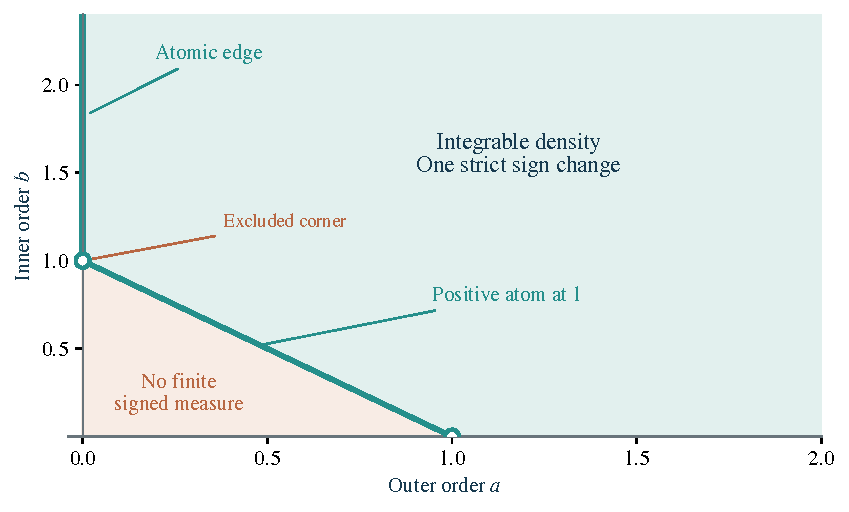
\includegraphics[width=0.8\linewidth]{figures/real_measure_domain.pdf}
\caption{The exact finite signed-measure domain for $a\ge0,b>0$.
The teal edges carry a positive atom at one. The point $(0,1)$ is
excluded, and the horizontal axis $b=0$ is outside the stated domain.
The entire positive quadrant has zero-free principal continuation by
Theorem~\ref{subpick:thm:global}; finite signed-moment existence has the
smaller domain shown here.}
\label{fig:measure-domain}
\end{figure}

\subsection{A regularized positive kernel}

Set
\begin{equation}\label{subunit:eq:q}
 q(t)=\frac1{1-e^{-t}}-\frac1t,\qquad t>0.
\end{equation}
The elementary identities
\[
 q(t)=\frac12+\frac12\coth(t/2)-\frac1t,
 \qquad
 q'(t)=\frac1{t^2}-\frac1{4\sinh^2(t/2)}>0
\]
give $1/2<q(t)<1$, because $\sinh(t/2)>t/2$ and the endpoint
limits are $1/2$ and $1$. In particular $q$ is positive, bounded and
strictly increasing. Also $q(t)=1/2+O(t)$ as $t\downarrow0$.

For later use put $k_v(T)=T^{v-1}/\Gamma(v)$ for $v>0$. The positive convolution satisfies
\begin{align}
 C_{a,b}(T)&=\frac1{\Gamma(a)\Gamma(b)}
 \int_0^T(T-t)^{a-1}t^{b-1}q(t)\,dt
 =k_{a+b}(T)\mathbb E[q(TV)],\quad V\sim\mathrm{Beta}(b,a),
 \label{rw:aux:Cbeta}\\
 \tfrac12 k_{a+b}(T)&<C_{a,b}(T)<k_{a+b}(T),
 \label{rw:aux:Cbounds}\\
 \int_0^\infty e^{-nT}C_{a,b}(T)\,dT
 &=n^{-a}\left(\zeta(b,n)-\frac{n^{1-b}}{b-1}\right)
       \quad(b\ne1).\label{rw:aux:CLaplace}
\end{align}
At $b=1$ the last expression is $n^{-a}(\log n-\psi(n))$.
These identities follow by absolutely convergent convolution integrals.

The classical Hurwitz integral and one elementary subtraction give
\begin{equation}\label{subunit:eq:hurwitz}
 \zeta(b,x)=\frac{x^{1-b}}{b-1}
 +\frac1{\Gamma(b)}\int_0^\infty
              e^{-xt}t^{b-1}q(t)\,dt,
 \qquad x>0,\ b>0,\ b\ne1.
\end{equation}
For $b>1$ this is obtained by splitting $1/(1-e^{-t})=1/t+q(t)$
in the usual Gamma integral. The integral involving $q$ is holomorphic
for $\Re b>0$, so the identity theorem extends the same formula to
$0<b<1$. This is analytic continuation of an absolutely convergent
regularized integral, not subtraction of two divergent real integrals.
The standard starting integral and recurrence are DLMF
25.11.25 and 25.11.4 \cite{intdist:DLMFHurwitz}. For $b=1$ the corresponding formula is
\begin{equation}\label{subunit:eq:digamma}
 \psi(x)=\log x-\int_0^\infty e^{-xt}q(t)\,dt,
\end{equation}
which is DLMF 5.9.13 \cite{rw:DLMFDigamma} and also follows by taking the finite part of
\eqref{subunit:eq:hurwitz} at $b=1$.

For $0<b<1$, we shall use $\zeta(b)<0$. Indeed the alternating
Dirichlet series $\eta(b)$ is positive, while
$\eta(b)=(1-2^{1-b})\zeta(b)$ and $1-2^{1-b}<0$.

\subsection{Explicit densities and their Laplace transforms}

Put $T=-\log u$ and $K_{a,b}(T)=\kappa_{a,b}(e^{-T})$. For
$a>0$, $a+b>1$ and $b\ne1$, define
\begin{align}\label{subunit:eq:generalK}
 K_{a,b}(T)={}&\frac{\zeta(b)T^{a-1}}{\Gamma(a)}
 -\frac{T^{a+b-2}}{(b-1)\Gamma(a+b-1)}\notag\\
 &-\frac1{\Gamma(a)\Gamma(b)}
    \int_0^T(T-t)^{a-1}t^{b-1}q(t)\,dt.
\end{align}
When $b>1$, an equivalent form is
\begin{equation}\label{subunit:eq:largeB}
 K_{a,b}(T)=\frac{\zeta(b)T^{a-1}}{\Gamma(a)}
 -\frac1{\Gamma(a)\Gamma(b)}
   \int_0^T\frac{(T-t)^{a-1}t^{b-1}}{1-e^{-t}}\,dt.
\end{equation}
At $b=1$, define
\begin{align}\label{subunit:eq:bOne}
 K_{a,1}(T)={}&\frac{T^{a-1}}{\Gamma(a)}
       \bigl(\gamma+\psi(a)-\log T\bigr)\notag\\
 &-\frac1{\Gamma(a)}\int_0^T(T-t)^{a-1}q(t)\,dt.
\end{align}
The Gamma factors and the term $\gamma+\psi(a)$ in this last formula
are essential; in particular it reduces at $a=1$ to
$K_{1,1}(T)=-\log(e^T-1)$, agreeing with the original signed kernel.

These functions are integrable against $e^{-T}\,dT$. At zero,
\eqref{subunit:eq:generalK} has only the integrable powers
$T^{a-1}$, $T^{a+b-2}$ and $O(T^{a+b-1})$; the logarithmic factor
in \eqref{subunit:eq:bOne} is likewise integrable for $a>0$.
At infinity all terms have at most polynomial times logarithmic growth.
For $b>1$, the integrability of the convolution in
\eqref{subunit:eq:largeB} at its lower endpoint uses $b>1$ explicitly.

By the Gamma integral and the convolution rule, the Laplace transform
of \eqref{subunit:eq:generalK} is
\begin{align*}
 \int_0^\infty e^{-nT}K_{a,b}(T)\,dT
  &=n^{-a}\left[\zeta(b)-\frac{n^{1-b}}{b-1}
     -\frac1{\Gamma(b)}\int_0^\infty
                         e^{-nt}t^{b-1}q(t)\,dt\right]\\
  &=n^{-a}\bigl(\zeta(b)-\zeta(b,n)\bigr)
   =\frac{H_{n-1}^{(b)}}{n^a}.
\end{align*}
Each convolution interchange is justified absolutely; $q$ is bounded
and the remaining factors have Gamma integrals. Formula
\eqref{subunit:eq:bOne} has Laplace transform
\[
 n^{-a}\left(\gamma+\log n-\int_0^\infty e^{-nt}q(t)\,dt\right)
 =n^{-a}(\gamma+\psi(n))=\frac{H_{n-1}}{n^a}.
\]
Here the Laplace transform of $T^{a-1}\log T$ is obtained by
differentiating the Gamma integral, justified by absolute integrability.
The substitution $u=e^{-T}$ changes $u^{n-1}\,du$ to
$e^{-nT}\,dT$, proving the desired moment normalization. In particular
$n=1$ gives total mass zero.

\subsection{The one-sign-change proof}

For $b>1$, divide \eqref{subunit:eq:largeB} by $T^{a-1}$ and
rescale $t=Tv$:
\[
 T^{1-a}K_{a,b}(T)=\frac{\zeta(b)}{\Gamma(a)}
 -\frac1{\Gamma(a)\Gamma(b)}
  \int_0^1(1-v)^{a-1}v^{b-1}\frac{T^b}{1-e^{-Tv}}\,dv.
\]
For fixed $v>0$, the logarithmic derivative of
$T^b/(1-e^{-Tv})$ is
\[
 \frac bT-\frac{v}{e^{Tv}-1}>\frac{b-1}{T}>0.
\]
Thus the rescaled density is strictly decreasing. Its limit at zero is
$\zeta(b)/\Gamma(a)>0$, and its limit at infinity is $-\infty$.
This proves one strict positive--negative crossing in the $T$ coordinate.

For $b=1$, the rescaled expression is
\[
 \Gamma(a)T^{1-a}K_{a,1}(T)
 =\gamma+\psi(a)-\log T
  -T\int_0^1(1-v)^{a-1}q(Tv)\,dv.
\]
It is strictly decreasing from $+\infty$ to $-\infty$, since $q$ is
positive and increasing. For $0<b<1$, instead divide by
$T^{a+b-2}$ to obtain
\begin{align}\label{subunit:eq:rescaledLowB}
 T^{2-a-b}K_{a,b}(T)={}&
 \frac1{(1-b)\Gamma(a+b-1)}
 +\frac{\zeta(b)}{\Gamma(a)}T^{1-b}\notag\\
 &-\frac{T}{\Gamma(a)\Gamma(b)}
   \int_0^1(1-v)^{a-1}v^{b-1}q(Tv)\,dv.
\end{align}
Now the first term is positive, the second is strictly decreasing
because $\zeta(b)<0$, and the final term is strictly decreasing because
$q$ is positive and increasing. The endpoint limits are a positive
constant and $-\infty$. Thus there is again exactly one strict crossing.
The derivatives of these rescaled expressions are strictly negative;
differentiation is dominated by the same integrable beta weights.
At a zero of $K$, multiplication by the positive rescaling factor does
not affect the sign of its derivative. Reversing $T=-\log u$ gives
the asserted negative--positive sign change and a strictly positive
$u$ derivative at its unique crossing.

\subsection{The critical atom and the exact boundary}

Let $0<b<1$ and $a=1-b$. Replace the middle term of
\eqref{subunit:eq:generalK} by an atom of mass $(1-b)^{-1}$ at $u=1$,
and retain the density
\begin{equation}\label{subunit:eq:criticaldensity}
 K_{1-b,b}(T)=\frac{\zeta(b)T^{-b}}{\Gamma(1-b)}
 -\frac1{\Gamma(1-b)\Gamma(b)}
   \int_0^T(T-t)^{-b}t^{b-1}q(t)\,dt.
\end{equation}
Both terms are strictly negative and integrable against $e^{-T}\,dT$.
Its moments plus the atom are
\[
 \frac1{1-b}+n^{b-1}\left[\zeta(b)
   -\frac1{\Gamma(b)}\int_0^\infty e^{-nt}t^{b-1}q(t)\,dt\right]
 =\frac{H_{n-1}^{(b)}}{n^{1-b}},
\]
by \eqref{subunit:eq:hurwitz}. Thus the measure has total mass zero,
and its negative mass is exactly $(1-b)^{-1}$.

For $a=0$, $b>1$, the formula is especially simple:
\begin{equation}\label{subunit:eq:aZero}
 \nu_{0,b}=\zeta(b)\delta_1+K_{0,b}(-\log u)\,du,
 \qquad K_{0,b}(T)=-\frac{T^{b-1}}{\Gamma(b)(1-e^{-T})}.
\end{equation}
The ordinary Hurwitz integral gives its moments immediately. Its
negative mass is exactly $\zeta(b)$.

Every finite signed measure has bounded moments, since
$|\int u^{n-1}\,d\nu|\leq\|\nu\|_{\mathrm{TV}}$.
If $0<b<1$, elementary integral comparison gives
$H_{n-1}^{(b)}\sim n^{1-b}/(1-b)$, so the moments diverge to
infinity when $a+b<1$. If $a=0,b=1$, they diverge logarithmically.
These are exactly the excluded cases for $a\geq0,b>0$.
Finally, two finite signed measures with the same moments integrate
every polynomial equally; polynomial density in $C([0,1])$ makes the
measures identical. This proves Theorem~\ref{subunit:thm:domain}.

\section{Consequences for complex zeros and angular zeros}

\begin{theorem}[Nonvanishing throughout the finite-measure domain]
\label{subunit:thm:zerofree}
For all parameters in \eqref{subunit:eq:domain}, $F_{a,b}$ has an
analytic continuation to $\mathbb C\setminus[1,\infty)$ and has no
zero there except for its double zero at the origin. Every upper
open semicircle $z=\rho e^{i\theta}$, $0<\rho\leq1$, $0<\theta<\pi$,
has exactly one
simple zero of $\operatorname{Im}F_{a,b}(z)$, and it satisfies
\[
 \arccos\rho<\theta_{a,b}(\rho)<\frac\pi2.
\]
The imaginary part is positive below this angle and negative above
it; its angular derivative at the zero is strictly negative.
In the atomic cases, unit-circle values mean analytic continuation
or Abel boundary values: the original Fourier summands do not tend
to zero, so ordinary Fourier convergence is not asserted.
\end{theorem}

\begin{proof}
The signed transform
\[
 F_{a,b}(z)=z\int_{[0,1]}\frac{d\nu_{a,b}(u)}{1-zu}
\]
follows by geometric expansion in the disk and extends analytically
to the slit plane by uniform domination on compact sets. Let $r$ be
the crossing from Theorem~\ref{subunit:thm:domain}, or let $r=1$ in
the atomic cases. Zero mass gives
\begin{equation}\label{subunit:eq:factor}
 F_{a,b}(z)=\frac{z^2}{1-rz}P_{a,b}(z),\qquad
 P_{a,b}(z)=\int_{[0,1]}\frac{u-r}{1-zu}\,d\nu_{a,b}(u).
\end{equation}
The measure $(u-r)\,d\nu_{a,b}(u)$ is positive and nonzero, including
when $r=1$: its atom disappears but its density is strictly positive
on $(0,1)$. Consequently $\operatorname{Im}P_{a,b}(z)$ has the
strict sign of $\operatorname{Im}z$, while $P_{a,b}(x)>0$ for
$x<1$. Apart from the explicit $z^2$, the factor $(1-rz)^{-1}$ in
\eqref{subunit:eq:factor} is analytic and nonzero on the slit plane. Since $P_{a,b}(0)=A_2=2^{-a}$,
the zero at zero has multiplicity exactly two.

For angular zeros put
\[
 J_\rho(c)=\int_{[0,1]}\frac{d\nu(u)}{1-2\rho cu+\rho^2u^2},
 \qquad
 \operatorname{Im}F(\rho e^{i\theta})
       =\rho\sin\theta\,J_\rho(\cos\theta).
\]
The zero-mass one-crossing sign test holds for our atomic measures as
well: subtract the value of the test function at $r$, and use the
ordered supports of the two signs. It gives $J_\rho(0)<0$.
When $\rho<1$, the kernel at $c=\rho$ is strictly increasing in $u$,
so $J_\rho(\rho)>0$. When $\rho=1$ and the crossing is interior,
separate the two signs before expanding $(1-u)^{-2}$ to obtain
\[
 \lim_{c\uparrow1}J_1(c)
 =\int_{[0,1]}\frac{d\nu(u)}{(1-u)^2}
 =\sum_{n\geq1}n A_n>0,
\]
allowing $+\infty$. The negative part is supported away from one, so
this is the same justified monotone-limit argument as in the original
signed-kernel theorem. In the atomic cases the limiting signed
integral at $c=1$ need not be defined, and we do not use that display.
Instead the limit is $+\infty$ directly: the atom contributes
$M/[2(1-c)]$, and the negative density contributes
$o((1-c)^{-1})$. For the latter assertion, multiply its integral by
$1-c$ and use dominated convergence: the multiplier
$(1-c)/(1-2cu+u^2)$ is bounded by $1$ for $0\leq c<1$ and tends to zero for
every $u<1$. The negative density is integrable and has no atom at one.

For $c'>c$, the quotient of the two kernels has derivative
\[
 \frac{d}{du}\frac{1-2\rho cu+\rho^2u^2}
                         {1-2\rho c'u+\rho^2u^2}
 =\frac{2\rho(c'-c)(1-\rho^2u^2)}
       {(1-2\rho c'u+\rho^2u^2)^2}>0\quad(0<u<1).
\]
At any zero, apply the sign test to the signed measure obtained by
weighting $\nu$ with the positive kernel. It follows that $J_\rho$
is positive at every larger $c$ and negative at every smaller $c$;
this proves uniqueness and the signs. Finally its derivative at its
zero is positive, because the additional factor
$2\rho u/(1-2\rho cu+\rho^2u^2)$ is strictly increasing in $u$.
The angular derivative is therefore
$-\rho\sin^2\theta\,J_\rho'(\cos\theta)<0$.
\end{proof}

\begin{corollary}[Ordinary and analytic boundary values]\label{rw:cor:boundary}
For $a,b>0$ with $a+b>1$, the defining series converges ordinarily
at every $|z|=1,z\ne1$, and equals its analytic continuation. At
$a+b\le1$, or on the axis $a=0,b>0$, its terms do not tend to zero
at those boundary points. There the stated values are analytic or Abel values.
\end{corollary}
\begin{proof}
In the absolutely continuous finite-measure case, expand the finite geometric
sum and use domination of $z(1-(zu)^N)/(1-zu)$ against the total variation;
there is no atom at one. Harmonic asymptotics give a positive nonzero limit
or unbounded coefficients in the remaining cases, so the term test fails.
The axis formula and the subsequent Stieltjes factorization still give
well-defined continuation and radial Abel limits away from the cut.
\end{proof}

\section{A positive two-variable representation at all positive orders}
\label{rw:sec:double}

The threshold in Theorem~\ref{subunit:thm:domain} concerns a
\emph{one-variable finite signed measure}. It is not a threshold for
analytic continuation or every positivity property.

\begin{theorem}[Positive double kernel]\label{rw:thm:double}
For every $a,b>0$ and $z\in\realcut$,
\begin{equation}\label{rw:eq:double}
 F_{a,b}(z)=z^2\int_{0<y<x<1}
 \frac{W_{a,b}(x,y)}{(1-xz)(1-yz)}\dd y\dd x,
\end{equation}
where
\begin{equation}\label{rw:eq:W}
 W_{a,b}(x,y)=\frac{(-\log x)^{a-1}(\log(x/y))^{b-1}}
 {\Gamma(a)\Gamma(b)}.
\end{equation}
The weight is strictly positive and has total mass $2^{-a}$.
\end{theorem}
\begin{proof}
For $|z|<1$, expand the two denominators. Substitution $y=xv$
gives, for nonnegative integers $j,k$,
\[
 \int_{0<y<x<1}W_{a,b}(x,y)x^jy^k\dd y\dd x
 =\frac1{(j+k+2)^a(k+1)^b}.
\]
Summing over $j+k=n-2$ yields $c_n$. Absolute convergence justifies
the rearrangement, and taking $j=k=0$ gives the total mass.
On each compact subset of $\realcut$, both denominators are bounded
away from zero uniformly in $x,y\in[0,1]$. The integral is consequently
holomorphic there and supplies the stated continuation.
\end{proof}

\begin{corollary}[Disk nonvanishing below and above the threshold]
\label{rw:cor:disk}
For all $a,b>0$, $F_{a,b}$ has no nonzero zeros in
$\{z:|z|\le1,\ z\ne1\}$. More precisely, when $\Imag z>0$ and
$|z|\le1$,
\begin{equation}\label{rw:eq:diskpick}
 \Imag\frac{F_{a,b}(z)}z>0.
\end{equation}
At any upper-half-disk zero of $\Imag F_{a,b}(z)$, the value
$F_{a,b}(z)$ itself is strictly negative real.
\end{corollary}
\begin{proof}
A direct calculation gives
\[
 \Imag\frac{z}{(1-xz)(1-yz)}
 =\frac{(\Imag z)(1-xy|z|^2)}{|1-xz|^2|1-yz|^2}>0
\]
for $0<y<x<1$, proving \eqref{rw:eq:diskpick}. The lower half follows
by conjugation. On the real interval $z<1$, the integral
$F(z)/z^2$ is strictly positive. Finally, if $F(z)=R\in\R$ with
$\Imag z>0$, then $\Imag(R/z)=-R\Imag z/|z|^2>0$, so $R<0$.
\end{proof}

\begin{corollary}[Gaussian negativity and strict log-convexity]
\label{rw:cor:gaussian}
For every $a,b>0$,
\begin{equation}\label{rw:eq:gaussianpositive}
 -g_{a,b}=\int_{0<y<x<1}W_{a,b}(x,y)
       \frac{x+y}{(1+x^2)(1+y^2)}\dd y\dd x>0,
\end{equation}
and
\begin{equation}\label{rw:eq:gaussianbounds}
 \frac{H_2^{(b)}}{4\,3^a}<-g_{a,b}<\frac{H_2^{(b)}}{3^a}.
\end{equation}
The function $(a,b)\mapsto\Gamma(a)\Gamma(b)(-g_{a,b})$ is strictly
log-convex on the positive quadrant.
\end{corollary}
\begin{proof}
Set $z=\iu$ in \eqref{rw:eq:double} and rationalize the denominator.
Since $1<(1+x^2)(1+y^2)<4$ and
$\int W(x+y)=c_3=H_2^{(b)}/3^a$, the bounds follow.
For log-convexity apply H\"older's inequality to the positive integral
with the gamma factors removed. Its parameter dependence is the
exponential of
$(a-1)\log(-\log x)+(b-1)\log\log(x/y)$.
Equality in H\"older would require a nontrivial real linear combination
of these two logarithms to be constant almost everywhere on the open
triangle, which is impossible. This proves strictness for every
nontrivial line segment of parameter pairs.
\end{proof}

\subsection{All-order integral identities}
\begin{theorem}[Hurwitz--polylogarithm transport]\label{rw:thm:transport}
For $a,b>0$, $b\ne1$, and $z\in\realcut$,
\begin{align}\label{rw:eq:transport}
 F_{a,b}(z)={}&\zeta(b)\Li_a(z)-\frac{\Li_{a+b-1}(z)}{b-1}\notag\\
 &-\frac1{\Gamma(b)}\int_0^\infty t^{b-1}q(t)\Li_a(ze^{-t})\dd t.
\end{align}
At $b=1$ the pole-free identity is
\begin{equation}\label{rw:eq:transport1}
 F_{a,1}(z)=\gamma\Li_a(z)-\partial_a\Li_a(z)
       -\int_0^\infty q(t)\Li_a(ze^{-t})\dd t.
\end{equation}
In particular, the index $a+b-1$ in \eqref{rw:eq:transport} is allowed
to be zero or negative.
\end{theorem}
\begin{proof}
Inside the disk, multiply \eqref{subunit:eq:hurwitz}, with $x=n$, by
$n^{-a}z^n$ and sum. Exponential decay at infinity, boundedness of
$q$, and $b>0$ justify termwise integration. The Hurwitz difference
is $H_{n-1}^{(b)}$, so coefficient comparison gives
\eqref{rw:eq:transport}. At $b=1$, use
$H_{n-1}=\gamma+\log n-\int_0^\infty e^{-nt}q(t)\dd t$;
the sum of $(\log n)n^{-a}z^n$ is $-\partial_a\Li_a(z)$.
The integral expressions on the right are locally holomorphic on the
slit plane. Near $t=0$, $\Li_a(ze^{-t})$ stays bounded on compact
slit sets, and at infinity it is $O(e^{-t})$. Analytic continuation
therefore proves the identities throughout the claimed domain.
Standard conventions for $\Li_s$ are those of DLMF 25.12
\cite{rw:DLMFPolylog}.
\end{proof}

These identities are useful even when no signed Hausdorff measure
exists. They are transformations to a depth-one polylogarithm integral,
not assertions that a depth-two constant has been reduced to a finite
basis of depth-one periods.

\section{Below the measure threshold: positive differences settle the zero question}
\label{subpick:sec:main}
The failure of finite signed-moment representability below $a+b=1$
does not imply a failure of positivity after a discrete derivative.
Consecutive differences supply a finite positive measure and resolve
the slit-plane nonvanishing and angular-uniqueness questions left open
by the real-order reports. They also extend the right-endpoint radial
mechanism from the critical line to the entire subcritical region.

Write $c_n=H_{n-1}^{(b)}/n^a$ and $F_{a,b}(z)=\sum_{n\ge1}c_nz^n$.
For $a>0$, $b>0$, $w=a+b<1$, put $s=w-1\in(-1,0)$ and
\begin{align}
 k_v(T)&=T^{v-1}/\Gamma(v),\\
 \mathfrak h(t)&=(1-e^{-t})^{-1}-t^{-1},\\
 \mathcal C_{a,b}(T)&=\frac1{\Gamma(a)\Gamma(b)}
  \int_0^T(T-t)^{a-1}t^{b-1}\mathfrak h(t)\,dt,\\
 R_{a,b}(T)&=-\zeta(b)k_a(T)-\frac{k_s(T)}{1-b}
                +\mathcal C_{a,b}(T).\label{subpick:eq:R}
\end{align}
Here $k_s$ is a signed function, not a positive Gamma density:
$\Gamma(s)=\Gamma(s+1)/s<0$. Since $0<b<1$, $\zeta(b)<0$,
and $1/2<\mathfrak h(t)<1$, all three terms of $R_{a,b}$ are
strictly positive. The regularized Hurwitz identity used here is
\[
 \zeta(b,n)=\frac{n^{1-b}}{b-1}
 +\frac1{\Gamma(b)}\int_0^\infty e^{-nt}t^{b-1}\mathfrak h(t)\,dt;
\]
it follows from the convergent Hurwitz integral by subtraction and
analytic continuation in $b$, as in the preceding construction
\cite{intdist:DLMFHurwitz}.

\begin{theorem}[Positive Hausdorff differences]
\label{subpick:thm:differences}
For $a,b>0$ with $a+b<1$, define
\[
 d\omega_{a,b}(u)=(1-u)R_{a,b}(-\log u)\,du,\qquad 0<u<1.
\]
This is a finite positive measure, with strictly positive density and
mass $2^{-a}$. For every $n\ge1$,
\begin{align}
 c_n&=\int_0^1(1-u^{n-1})R_{a,b}(-\log u)\,du,
       \label{subpick:eq:bernstein}\\
 c_{n+1}-c_n&=\int_0^1u^{n-1}\,d\omega_{a,b}(u).
       \label{subpick:eq:differences}
\end{align}
The first measure has infinite mass, but every displayed integral is
absolutely convergent. Thus the shifted sequence $c_{n+1}$ is a discrete
Bernstein sequence, and its differences are strictly completely monotone.
Here $\Delta f_n=f_{n+1}-f_n$. In particular, for all $j\ge0$ and $n\ge1$,
\[
 (-1)^j\Delta^j(c_{n+1}-c_n)
   =\int_0^1u^{n-1}(1-u)^j\,d\omega_{a,b}(u)>0.
\]
The positive difference measure is uniquely determined by these moments.
\end{theorem}
\begin{proof}
At $T=0$, the leading term of $R$ is a positive constant times
$T^{w-2}$; the other terms have orders $T^{a-1}$ and $T^{w-1}$.
Multiplication by $1-e^{-T}$ therefore makes it integrable, since
$w>0$. At infinity all terms grow at most polynomially and the change
of variables $u=e^{-T}$ supplies $e^{-T}$. This proves finiteness of
$\omega$, convergence of \eqref{subpick:eq:bernstein}, and divergence
of the unweighted mass at $u=1$.

For $s\in(-1,0)$, integration by parts gives the convergent identity
\[
 \int_0^\infty(e^{-T}-e^{-nT})k_s(T)\,dT=1-n^{-s}.
\]
Both boundary terms vanish: near zero their order is $T^{s+1}$,
and infinity has exponential decay. For $k_a$ the same identity is
the ordinary Gamma integral. The convolution has Laplace transform
\[
 \int_0^\infty e^{-nT}\mathcal C_{a,b}(T)\,dT
 =n^{-a}\left(\zeta(b,n)+\frac{n^{1-b}}{1-b}\right).
\]
Every convolution interchange is absolute. Insert these three identities
into \eqref{subpick:eq:R}, with the factor $e^{-T}-e^{-nT}$ retained.
The constant and power terms cancel, leaving
$n^{-a}(\zeta(b)-\zeta(b,n))=c_n$. No divergent Laplace transforms
are subtracted. Subtract the two convergent formulas at $n+1$ and $n$
to obtain \eqref{subpick:eq:differences}. At $n=1$ this gives mass
$c_2=2^{-a}$. The difference formula proves every strict sign, and
polynomial density on $[0,1]$ proves uniqueness of the finite measure.
\end{proof}

On the critical line $a=1-b>0$, use instead
$R_{a,b}=-\zeta(b)k_a+\mathcal C_{a,b}$. Its finite mass is $1/a$,
and its Laplace transform is $1/a-c_n$, so the same formulas for
$\omega=(1-u)R(-\log u)\,du$ hold. This is precisely the negative
density of the critical signed measure; its positive atom at one
disappears after multiplication by $1-u$.
On the whole axis $a=0,b>0$, the difference measure is simply
\[
 d\omega_{0,b}(u)=\frac{(-\log u)^{b-1}}{\Gamma(b)}\,du,
 \qquad c_{n+1}-c_n=n^{-b},
\]
and $F_{0,b}(z)=z\Li_b(z)/(1-z)$. These measures also have strictly
positive densities, with mass $2^{-a}$ and no endpoint atoms.

\begin{corollary}[A sharp complementary positivity classification]
\label{subpick:cor:classification}
For $a\ge0,b>0$, the consecutive differences $c_{n+1}-c_n$ are
moments of a finite positive measure on $[0,1]$ if and only if
$a=0$ or $a+b\le1$. In the same parameter region the function
\[
 \Phi_{a,b}(t)=(t+1)^{-a}
       \{\zeta(b)-\zeta(b,t+1)\},\qquad t\ge0,
\]
with $\gamma+\psi(t+1)$ replacing the braces at $b=1$, is a
Bernstein function: $\Phi(0)=0$, $\Phi(t)>0$ for $t>0$, and
$(-1)^j\Phi^{(j+1)}(t)>0$ for all $j\ge0$.
\end{corollary}
\begin{proof}
The preceding proof works for every real $n\ge1$, since the Gamma
and regularized Hurwitz identities used there do not require integer
$n$. Thus $\Phi(t)=\int(1-u^t)\,d\rho(u)$ with
$d\rho=d\omega/(1-u)$. Differentiation gives
\[
 (-1)^j\Phi^{(j+1)}(t)
   =\int_0^1(-\log u)^{j+1}u^t\,d\rho(u)>0.
\]
All these integrals converge even at $t=0$: the endpoint at one is
controlled by $\int(1-u)\,d\rho<\infty$, and the logarithmic-coordinate
density at zero has exponential decay times polynomial growth.
The same representation follows on the axis from the ordinary Hurwitz
integral, or its convergent difference at $b\le1$.

Conversely, for $a>0,a+b>1$, elementary harmonic asymptotics give
$c_n\to0$ while $c_2=2^{-a}>0$. The sequence cannot be nondecreasing,
so its differences cannot all be positive-measure moments and its
continuous interpolation cannot be a Bernstein function. This proves
both sharp parameter statements.
\end{proof}

\begin{theorem}[Global nonvanishing at all positive inner orders]
\label{subpick:thm:global}
For every $a\ge0$, $b>0$, the principal continuation of $F_{a,b}$
has no zero on $\C\setminus[1,\infty)$ except its double zero at zero.
For $a>0$, $a+b\le1$, and also for $a=0,b>0$, the stronger factorization is
\begin{equation}\label{subpick:eq:factor}
 F_{a,b}(z)=\frac{z^2}{1-z}P_{a,b}(z),\qquad
 P_{a,b}(z)=\int_0^1\frac{d\omega_{a,b}(u)}{1-zu}.
\end{equation}
In particular $P(0)=2^{-a}$, $\Imag P(z)$ has the strict sign of
$\Imag z$, and $P(x)>0$ for every real $x<1$.
\end{theorem}
\begin{proof}
The coefficient of $z^m$ in $(1-z)F(z)/z^2$ is
$c_{m+2}-c_{m+1}$, including $m=0$ because $c_1=0$.
The difference moments give \eqref{subpick:eq:factor} in the disk.
The finite positive measure gives holomorphic continuation to the slit
plane, where its imaginary-part and real-axis signs prove nonvanishing.
The mass proves multiplicity exactly two. For $a>0,a+b>1$, the
one-crossing finite signed measure already gives
$F=z^2P_r/(1-rz)$ with a nonzero positive Stieltjes transform and
$0<r<1$. The same argument applies. This proves the complete parameter
statement while retaining the sharp boundary for finite signed moments.
\end{proof}

\subsection{Angular uniqueness and a full subcritical radial theorem}
\begin{theorem}[Right-endpoint Stieltjes geometry]
\label{subpick:thm:radial}
For $a,b>0$ with $a+b\le1$, and for $a=0,b>0$, every open upper
semicircle of radius $0<\rho\le1$ has exactly one simple zero of
$\Imag F_{a,b}$. Its angle satisfies
\[
 \arccos\rho<\theta_{a,b}(\rho)<\arccos(\rho/2),
 \qquad \tfrac12<\eta_{a,b}(\rho)=\cos\theta_{a,b}(\rho)/\rho<1.
\]
The imaginary part is positive before that angle and negative after it.
The normalized quantity $\eta_{a,b}$ is strictly increasing in $\rho$.
Together with the supercritical angular theorem, this proves angular
uniqueness for every $a\ge0,b>0$, including the formerly conjectural
subcritical region. Boundary values are analytic or Abel values where
the ordinary Fourier series does not converge.
\end{theorem}
\begin{proof}
The following argument works for any finite positive measure $\omega$
with a strictly positive density on $(0,1)$. Set $x=\rho^2$,
$m=2\cos\theta/\rho-1$, and
\[
 D(u)=1+x\{u^2-(1+m)u\},\qquad
 G(m,x)=\int_0^1\frac{m-u}{D(u)}\,d\omega(u).
\]
From \eqref{subpick:eq:factor}, direct rationalization gives
\[
 \Imag F(\rho e^{i\theta})
  =\frac{\rho^3\sin\theta}{|1-\rho e^{i\theta}|^2}G(m,x).
\]
For $0<m<1$ all denominators are positive, and
\[
 G_m=\int_0^1\frac{1-xu}{D(u)^2}\,d\omega(u)>0.
\]
We have $G(0,x)<0$. For $x<1$, $G(1,x)>0$.
At $x=1$, its negative part for $u>m\ge1/2$ is bounded in magnitude
by $2\omega((m,1))$, which tends to zero. Its positive part tends
pointwise to $d\omega(u)/(1-u)$ and has a strictly positive limit
inferior by Fatou's lemma, with infinity allowed. Hence $G(m,1)>0$
for some $m<1$. This proves a unique root in $(0,1)$ even when
$\omega/(1-u)$ has infinite mass. Outside that interval the numerator
has a fixed sign, proving uniqueness on the full upper arc.
At the zero, the angular derivative is
$-2\rho^2\sin^2\theta\,G_m/|1-\rho e^{i\theta}|^2<0$.

At a root, the probability measure proportional to $d\omega/D$ has
mean $m$. For $d(u)=u^2-(1+m)u$, the identities
$d(m)=-m$ and $d(u)-d(m)=(u-m)(u-1)$ give
\[
 G_x=-\frac1{1-xm}\int_0^1
                 \frac{(u-m)^2(1-u)}{D(u)^2}\,d\omega(u)<0.
\]
Consequently
\[
 \frac{dm}{dx}
 =\frac{\displaystyle\int (u-m)^2(1-u)D(u)^{-2}\,d\omega(u)}
 {(1-xm)\displaystyle\int(1-xu)D(u)^{-2}\,d\omega(u)}>0,
 \qquad \eta'(\rho)=\rho m'(\rho^2)>0.
\]
All differentiations are dominated locally at the interior root,
including at $x=1$ since $m<1$. The implicit-function theorem proves
smooth dependence. This argument uses only the finite measure $\omega$;
it does not apply a finite-measure limit theorem to its infinite
unweighted predecessor.
\end{proof}

\subsection{One-sided Euler certificates even for divergent boundary series}
\begin{theorem}[Subcritical Euler continuation and a sharp fixed-pair constant]
\label{subpick:thm:euler}
For the parameters of Theorem~\ref{subpick:thm:radial}, put
$A_k=c_{2k+1}$, $g_{a,b}=\Imag F_{a,b}(i)$ and
\[
 E_N=\sum_{j=0}^{N-1}2^{-j-1}
             \sum_{k=0}^j(-1)^k\binom jk A_k.
\]
Then $E_N$ decreases strictly to the analytic Gaussian value, and
\begin{align}
 -g_{a,b}&=\frac12\int_0^1\frac{1+u}{1+u^2}\,d\omega(u),\\
 E_N-g_{a,b}&=2^{-N}\int_0^1
       \frac{(1+u)(1-u^2)^{N-1}}{1+u^2}\,d\omega(u)>0.
       \label{subpick:eq:euler-tail}
\end{align}
The least constant in $E_N-g\le C2^{-N}$ for all $N\ge1$ is
$C=-2g$, and
\[
 2^{-a}<-2g_{a,b}<\frac{1+\sqrt2}{2}\,2^{-a}<\frac54.
\]
Thus $E_N-(5/4)2^{-N}<g_{a,b}<E_N$ is a rational enclosure throughout
this domain. It concerns analytic continuation when the ordinary
alternating series diverges.
\end{theorem}
\begin{proof}
For $j\ge1$, the finite binomial difference of $A_k$ is
\[
 -\int_0^1(1+u)(1-u^2)^{j-1}\,d\omega(u),
\]
while the order-zero difference is $A_0=0$. Sum the geometric tail
against the finite measure to get \eqref{subpick:eq:euler-tail}.
Evaluating \eqref{subpick:eq:factor} at $i$ gives the same limiting
value. The scaled errors decrease strictly to zero, and their largest
value is $2(E_1-g)=-2g$. Finally $(1+u)/(1+u^2)$ has minimum one
at the endpoints and maximum $(1+\sqrt2)/2$ at $u=\sqrt2-1$.
The positive density makes both bounds strict, and the measure has
mass $2^{-a}$. Since $\sqrt2<3/2$, the rational bound follows.
\end{proof}

The global integer-outer-order normalized-radius conjecture remains open.
The new radial theorem covers the full subcritical and critical region
and the zero outer-order axis; it does not assert the same radial
direction in the supercritical region, where fractional turning points
are possible. Finite signed-moment existence, analytic nonvanishing,
angular uniqueness and radial motion now have explicitly different scopes.

\begin{corollary}[An exact Gaussian identity on the outer-order axis]
\label{subpick:cor:axis}
For every $b>0$, with analytic or Abel interpretation when necessary,
\[
 g_{0,b}=-\frac12\left(\beta(b)+2^{-b}\eta(b)\right),
 \qquad \eta(b)=\sum_{n\ge1}\frac{(-1)^{n-1}}{n^b}.
\]
In particular $g_{0,1}=-\pi/8-\log2/4$ and
$g_{0,2}=-G/2-\pi^2/96$.
\end{corollary}
\begin{proof}
The defining residue classes give
$\Li_b(i)=-2^{-b}\eta(b)+i\beta(b)$. Since
$F_{0,b}(i)=i\Li_b(i)/(1-i)=(-1+i)\Li_b(i)/2$,
its imaginary part is the claimed expression. Both Dirichlet series
converge for $b>0$; the depth-two series retains its stated boundary
interpretation. These formulas also identify the sharp fixed-pair
Euler constant as $\beta(b)+2^{-b}\eta(b)$ on this axis.
\end{proof}

\begin{theorem}[Strict Gaussian decrease in the real outer order]
\label{subpick:thm:Gaussian-order}
For every fixed $b>0$, the positive magnitude $-g_{a,b}$ decreases
strictly as $a$ runs through $[0,\infty)$. In particular, for $a>0$,
\[
 0<-2g_{a,b}<\beta(b)+2^{-b}\eta(b)<\frac{1+\sqrt2}{2}.
\]
The supremum over nonnegative outer orders is the explicit axis value.
This is a magnitude bound; it is not an Euler remainder constant in
parameter regions where the right-endpoint Stieltjes factorization
does not apply.
\end{theorem}
\begin{proof}
The outer Gamma integral, first by coefficient comparison in the disk
and then by locally dominated continuation to the slit plane, is
\[
 F_{a,b}(z)=\frac1{\Gamma(a)}\int_0^\infty
                      t^{a-1}F_{0,b}(ze^{-t})\,dt\qquad(a>0).
\]
Near zero its boundary value at $z=i$ is bounded; at infinity the
integrand without $t^{a-1}$ is $O(e^{-2t})$. Let
$h_b(t)=e^t[-\Imag F_{0,b}(ie^{-t})]$. The positive axis measure gives,
with $\rho=e^{-t}$,
\[
 h_b(t)=\int_0^1
  \frac{(1+u)\rho^2}{(1+\rho^2)(1+u^2\rho^2)}\,d\omega_{0,b}(u).
\]
The derivative in $\rho$ of the displayed kernel is
\[
 \frac{2\rho(1+u)(1-u^2\rho^4)}
 {(1+\rho^2)^2(1+u^2\rho^2)^2}>0\qquad(0<\rho\le1,\ 0<u<1).
\]
Thus $h_b$ is positive, bounded and strictly decreasing in $t$.
The Gamma integral is equivalently
$-g_{a,b}=\mathbb E[h_b(T_a)]$, where $T_a\sim\mathrm{Gamma}(a,1)$.
Independent Gamma variables satisfy $T_{a+d}\overset{d}=T_a+T_d$;
strict decrease of $h_b$ proves strict decrease of the expectation.
At $a=0$ take $T_0=0$, and bounded continuity gives the same strict
comparison and the limit as $a\downarrow0$.
For $a>0$, differentiation also gives the exact negative covariance
$\partial_a(-g_{a,b})=\Cov(\log T_a,h_b(T_a))<0$.
The axis identity and its positive-measure bound complete the proof.
\end{proof}

\begin{theorem}[Gaussian monotonicity at every fixed total order]
\label{subpick:thm:fixed-total}
For every $w>0$, $a\mapsto-2g_{a,w-a}$ decreases strictly on $(0,w)$.
Its endpoint limits give the exact strict inequalities
\[
 2\{\beta(w)-\beta(w-1)\}
 <-2g_{a,w-a}<\beta(w)+2^{-w}\eta(w).
\]
Here $\beta(w-1)$ uses analytic continuation when necessary.
In particular, this proves the previously conjectural strict decrease
on the entire critical line $w=1$.
\end{theorem}
\begin{proof}
In the positive double kernel put $x=e^{-s}$, $y=e^{-(s+t)}$,
then $T=s+t$ and $R=s/T$. Its Gaussian value becomes
\[
 -g_{a,b}=\mathbb E[K(R,T)],\qquad
 K(R,T)=\frac{X(X+Y)}{(1+X^2)(1+Y^2)},\quad
 X=e^{-RT},\quad Y=e^{-T},
\]
where $T\sim\mathrm{Gamma}(w,1)$ and $R\sim\mathrm{Beta}(a,w-a)$
are independent. The Jacobian gives $e^{-2s-t}=e^{-T}X$;
the remaining power is $T^{w-1}$, so every normalization is explicit.
For fixed $T>0$ the derivative with respect to $X$ is
\[
 \frac{2X+Y-YX^2}{(1+X^2)^2(1+Y^2)}>0.
\]
Thus $K$ decreases strictly in $R$. The beta score along fixed $w$
is an increasing function of $R$, namely $\log(R/(1-R))$ minus
its mean. Differentiation therefore gives a strictly negative covariance.
All logarithmic beta moments are finite for $0<a<w$.
At $a\downarrow0$, $R\to0$ in probability; at $a\uparrow w$,
$R\to1$. Bounded convergence gives the two endpoint values. The
first is the axis formula. The second also follows from
$F_{w,0}(z)=\Li_{w-1}(z)-\Li_w(z)$ and its analytic value at $i$.
\end{proof}

\subsection{A unique global Gaussian maximum and the sharp critical Euler constant}
Put $C(b)=\beta(b)+2^{-b}\eta(b)$ and
$\phi(T)=(1+e^{-T})/(1+e^{-2T})$.
The axis measure gives $C(b)=\mathbb E[\phi(T_b)]$ for
$T_b\sim\mathrm{Gamma}(b,1)$. The function $\phi$ increases and then
decreases, with its unique maximum at $T=\log(1+\sqrt2)$.

\begin{theorem}[A unique, nondegenerate axis maximum]
\label{subpick:thm:axis-maximum}
The function $C$ has exactly one stationary point $b_*$ on $(0,\infty)$.
It is a nondegenerate global maximum; $C'>0$ below $b_*$ and $C'<0$
above it. Moreover,
\[
 1<b_*<2,\qquad \frac{227}{200}<C(b_*)<\frac{1+\sqrt2}{2}.
\]
The supremum of $-2g_{a,b}$ over $a\ge0,b>0$ is this maximum,
attained only at $(a,b)=(0,b_*)$. Over $a,b>0$ it is a supremum
approached at the same axis point.
\end{theorem}
\begin{proof}
The gamma law tends to zero in probability as $b\downarrow0$ and
to infinity in probability as $b\to\infty$. Hence $C(b)\to1$ at
both ends. For every finite $b>0$, $1<C(b)<\max\phi$, since the
density is positive throughout $(0,\infty)$. Thus an interior maximum exists.

We prove a strict two-intersection property. For
$1<\lambda<\max\phi$, the function
$f(T)=\phi(T)-\lambda$ has sign pattern negative, positive, negative,
with exactly two sign changes $T_1<T_2$. If $C(b_i)=\lambda$ at
three distinct orders $b_1<b_2<b_3$, each of the three integrals
$\int f(T)T^{b_i-1}e^{-T}\,dT$ vanishes. Write
$v=T^{b_2-b_1}$ and $p=(b_3-b_1)/(b_2-b_1)>1$.
Subtract from $v^p$ its secant line through the values at $T_1,T_2$,
and multiply by $-T^{b_1-1}$. Strict convexity gives a linear
combination of the three powers with the same sign pattern as $f$.
Its integral against $f(T)e^{-T}$ is strictly positive, contradicting
the three vanishing integrals. Thus every horizontal level has at most
two intersections.

At a stationary point $b_0$, take $\lambda=C(b_0)$. If also
$C''(b_0)=0$, the Mellin integral and its first two derivatives
vanish there. Their linear combination with kernel
$-T^{b_0-1}(\log T-\log T_1)(\log T-\log T_2)$ again has strictly
positive integral, a contradiction. Therefore every stationary point
is nondegenerate. It cannot be a local minimum: the end limits one,
the minimum itself, and the two adjacent larger values would give
three distinct intersections with its own horizontal level. Every
stationary point is consequently a strict maximum, and there can be
only one. This proves both derivative signs and nondegeneracy.

The exact axis certificate at $b=3/2$ gives $C(3/2)>227/200$.
For comparison, $\pi<22/7$ and $\log2<25/36$ give
$C(1)<571/504<227/200$. The latter logarithmic bound follows by
summing the first two terms of its artanh series and bounding the
remaining positive geometric tail. Also the first five terms of the
alternating Catalan series give $G<37/40$, hence
$C(2)=G+\pi^2/48<37/40+121/588<227/200$.
Strict unimodality now forces $1<b_*<2$. The magnitude theorem proves
the remaining supremum assertions.
\end{proof}

The numerical axis experiment finds
$b_*\approx1.30221658710124120959$ and
$C(b_*)\approx1.13656110333950956095$. These decimal locations are
diagnostics; the proved enclosure is $1<b_*<2$ and the preceding
exact value bounds. The uniqueness argument does not rely on a scan
or the numerical stationary-point solver.

\begin{corollary}[The sharp uniform constant on and below the critical line]
\label{subpick:cor:sharp-critical}
For every $a,b>0$ with $a+b\le1$ and every integer $N\ge1$,
\[
 0<E_N-g_{a,b}<C_{\mathrm{critical}}2^{-N},\qquad
 C_{\mathrm{critical}}=\frac\pi4+\frac{\log2}{2}.
\]
This is the least constant uniform over the critical line and is also
the least constant uniform over the whole positive subcritical triangle.
Thus the critical constant conjecture and its stronger strict-monotonicity
claim are both settled. The rational choice $57/50$ is valid on this triangle.
\end{corollary}
\begin{proof}
On the critical line, Theorem~\ref{subpick:thm:fixed-total} bounds
$-2g$ strictly by its left endpoint $C(1)=C_{\mathrm{critical}}$.
For $a+b<1$, the outer-order magnitude theorem gives
$-2g_{a,b}<C(b)$, and $b<1<b_*$ gives $C(b)<C(1)$.
Apply the fixed-pair Euler constant theorem. Sharpness follows from
the critical endpoint limit $a\downarrow0,b\uparrow1$ and the error
at $N=1$, where $E_1=0$. Finally $C(1)<571/504<57/50$.
The conclusion does not extend the same bound to arbitrary supercritical
orders or to the entire outer-order axis.
\end{proof}

\begin{figure}[htbp]
\centering
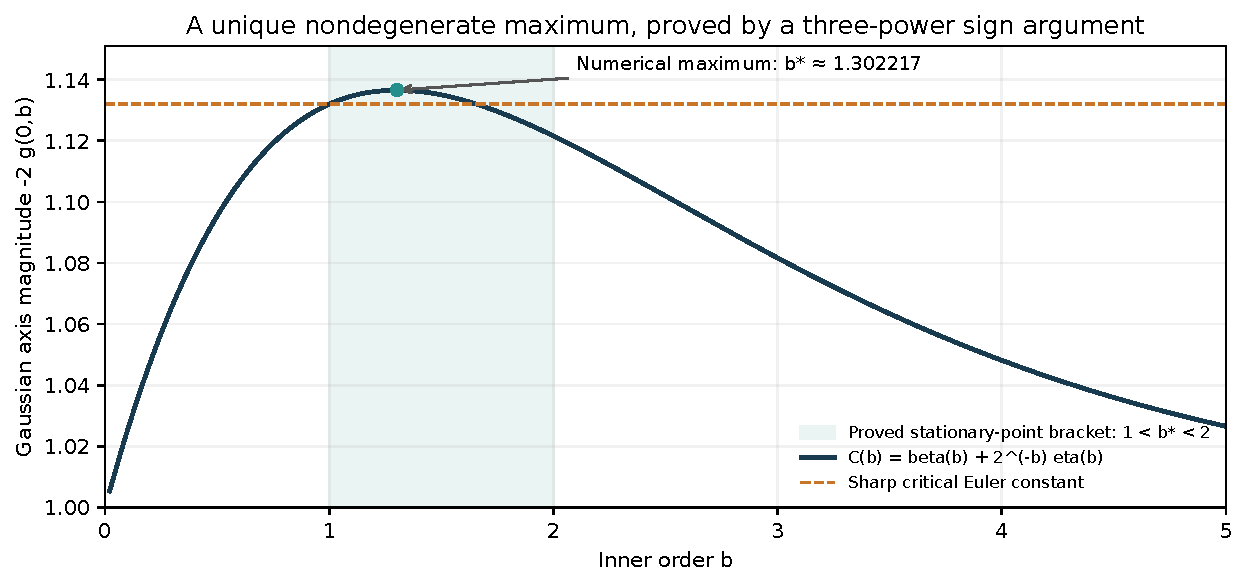
\includegraphics[width=\textwidth]{figures/Gaussian_axis_maximum.pdf}
\caption{Numerical values of the exact Gaussian axis expression and its
stationary-point marker. The shaded interval is the proved bracket for
the unique maximum; the horizontal line is the proved sharp critical
Euler constant. The maximum's displayed decimal location is diagnostic.
The larger global Gaussian maximum does not supply a universal Euler
constant in arbitrary supercritical parameter regions.}
\label{subpick:fig:Gaussian-axis}
\end{figure}

\section{Strict Gaussian envelope shape and a certified maximum}
\label{envref:sec:main}
The incoming extremal continuation~\cite{envref:report} independently
develops the axis maximum and strengthens its description. Its strict
normalized Mellin comparison gives a second proof of unimodality, Turan
inequalities and a rigorous enclosure of the maximum. We retain the
earlier three-power proof as a distinct route and reconcile the common
axis normalization before using the stronger certificate.

\begin{lemma}[A strict normalized Mellin comparison]\label{envref:lem:Mellin}
Suppose $f:(0,\infty)\to(0,\infty)$ is strictly log-concave, and that
its Mellin integrals and their first two parameter derivatives are finite
and admit differentiation under the integral. Then
\[
 M(p)=\frac1{\Gamma(p)}\int_0^\infty T^{p-1}f(T)\,dT\quad(p>0)
 \quad\text{satisfies}\quad (\log M)''(p)<0.
\]
\end{lemma}
\begin{proof}
Normalize $T^{p-1}f(T)$ to a probability density $P$. Choose the gamma
density $Q$ of shape $p$ and rate $\lambda>0$ so that
$\psi(p)-\log\lambda=\mathbb E_P\log T$.
The two densities have matching mass and matching logarithmic mean.
Their log likelihood ratio is $\log f(T)+\lambda T$ plus a constant,
hence strictly concave. Its positive set is an interval, and matching
mass forces both signs. A single crossing at $T_0$ is impossible:
$\log(T/T_0)(P-Q)$ would have one strict sign while its integral is
zero by the two matching moments. There must therefore be two crossings
$T_1<T_2$ and the sign pattern of $P-Q$ is negative, positive, negative.

It follows that
\[
 \int(\log T-\log T_1)(\log T-\log T_2)(P-Q)(T)\,dT<0.
\]
The constant and linear terms vanish by the matching moments. Thus
$\operatorname{Var}_P(\log T)<\operatorname{Var}_Q(\log T)=\psi_1(p)$.
Differentiation of $\log M$ gives exactly this variance difference.
\end{proof}

\begin{theorem}[Strict envelope log-concavity]\label{envref:thm:shape}
Put $D(b)=C(b)-1$, with $C$ defined in
Theorem~\ref{subpick:thm:axis-maximum}. For every $b>0$,
\[
 D(b)>0,\qquad (\log D)''(b)<0.
\]
Consequently $D(b)^2>D(b-h)D(b+h)$ for $0<h<b$.
Moreover $2^bD(b)$ increases strictly from zero to one.
\end{theorem}
\begin{proof}
Subtract the ordinary gamma integral for one from the axis integral:
\[
 D(b)=\frac1{\Gamma(b)}\int_0^\infty T^{b-1}f(T)\,dT,
 \qquad f(T)=\frac{e^{-T}(1-e^{-T})}{2\cosh T}.
\]
Here $f(T)=T/2+O(T^2)$ near zero, $f(T)<e^{-2T}$ at infinity, and
\[
 (\log f)''(T)=-\frac{e^T}{(e^T-1)^2}-\operatorname{sech}^2T<0.
\]
All differentiated integrals are locally dominated on $b>0$, so the
lemma applies. Strict midpoint concavity gives the Turan inequality.
The endpoint limits $D(b)\to0$ at zero and infinity also give a second
proof of a unique nondegenerate maximum: at its stationary point
$D''=D(\log D)''<0$.

For the final assertion let $T_b$ have gamma shape $b$ and rate two.
Then
\[
 2^bD(b)=\mathbb E\frac{1-e^{-T_b}}{1+e^{-2T_b}}.
\]
The displayed function increases strictly from zero to one. Gamma
addition gives strict increase with $b$. The gamma laws tend to zero
and infinity in probability at the respective parameter endpoints;
bounded convergence proves the limits.
\end{proof}

For example, the Turan inequality at $b=2,h=1$ gives the explicit
constant comparison
\[
 \left(G+\frac{\pi^2}{48}-1\right)^2>
 \left(\frac\pi4+\frac{\log2}{2}-1\right)
 \left(\frac{\pi^3}{32}+\frac{3\zeta(3)}{32}-1\right).
\]

\subsection{Outward rational enclosure of the axis maximum}
\begin{theorem}[Certified location and height]\label{envref:thm:certificate}
The unique maximum satisfies the rational inequalities
\begin{gather*}
 1.30221658710124120959237170<b_*<1.30221658710124120959237171,\\
 1.136561103339509560952586375779942387681723540
 <C(b_*)\\
 C(b_*)<1.136561103339509560952586375779942387681723541.
\end{gather*}
In particular $C(b_*)<57/50$.
\end{theorem}
\begin{proof}
The incoming standard-library verifier
\src{code/certify_gaussian_envelope.py} was replayed on an isolated copy.
We give the analytic budgets used in its finite certificate, so its
transcendental enclosures have explicit proof premises.
For $d=1,2$, put
\[
 A_d(b)=\sum_{j\ge0}\frac{(-1)^j}{(dj+1)^b},\qquad
 T_{d,N}(b)=2^{-N}\sum_{j=0}^{N-1}\frac{(-1)^j}{(dj+1)^b}
                          \sum_{h=j+1}^N\binom Nh.
\]
These give $A_1=\eta$ and $A_2=\beta$. For $T$ with gamma shape $b$
and rate one, finite geometric summation gives
\[
 A_d-T_{d,N}=2^{-N}\mathbb E
             \frac{(1-e^{-dT})^N}{1+e^{-dT}}\in(0,2^{-N}).
\]
Differentiating the gamma density introduces the centered score
$\log T-\psi(b)$. Cauchy--Schwarz and
$\sqrt{\psi_1(b)}\le\pi/\sqrt6<2$ for $b\ge1$ yield
$|A_d'-T_{d,N}'|<2^{1-N}$.
For $C_N=T_{2,N}+2^{-b}T_{1,N}$ this proves
\[
 0<C-C_N\le(1+2^{-b})2^{-N},\qquad
 |C'-C_N'|<4\,2^{-N}\quad(1\le b\le2).
\]

The finite terms are enclosed on an outward-rounded $10^{90}$ grid.
After reducing an integer logarithm to $1\le r\le2$, its expansion
\[
 \log r=2\sum_{j=0}^{M-1}\frac{v^{2j+1}}{2j+1}+R_M,
 \quad v=\frac{r-1}{r+1},\quad
 0\le R_M\le\frac{2v^{2M+1}}{(2M+1)(1-v^2)}
\]
uses $M=160$. Exponentials are scaled to $[0,1]$, bounded by their
positive Taylor polynomial through degree 180 and twice the first
omitted term, then recovered by four outward-rounded squarings and
positive reciprocals. Multiplication by the logarithm gives the
derivative enclosure with the same rational arithmetic.

With $N=160$, the resulting certificate proves $C'(\ell)>0$ and
$C'(u)<0$ at the displayed location endpoints. Its separate checks
give $C'(1)>0.03260$ and $C'(2)<-0.03561$.
Strict log-concavity of $D$ provides the tangent upper bound
\[
 D(b_*)\le D(\ell)
    \exp\left(\frac{C'(\ell)}{D(\ell)}(u-\ell)\right).
\]
The outward upper endpoint of this expression and the lower bound
$C(\ell)$ give the displayed value interval. The fresh exact receipt is
\src{verification/fifth-replay/extremal/results/gaussian_envelope_certificate.json}.
The final comparison with $57/50$ is rational. No numerical optimizer
or floating-point library evaluation is a premise.
\end{proof}

The old plotted stationary-point marker remains a diagnostic. The
enclosures above now certify its location and the axis height to the
displayed widths; they do not certify every plotted value.
The further inverse generalized-power expansion in the incoming report
is retained as a separate analytic integration task.

\section{Cartesian motion of the complete real-order zero arc}
\label{rwcart:sec:motion}
The normalized radial motion can have different signs above the critical
line, but its Cartesian abscissa has one direction throughout the entire
nonnegative-outer-order domain.

\begin{theorem}[Strict outward abscissa motion]
\label{rwcart:thm:motion}
For every $a\ge0,b>0$, put $s=\rho^2$ and
$X_{a,b}(s)=\rho\cos\theta_{a,b}(\rho)$. The unique upper-arc zero
has a real-analytic abscissa on $(0,1]$, extending real analytically
through zero, with
\[
 0<X_{a,b}(s)<s,\qquad X_{a,b}'(s)>0\quad(0<s\le1).
\]
This is an abscissa theorem; it does not assert one direction for
$\cos\theta/\rho$ in every supercritical parameter pair.
\end{theorem}
\begin{proof}
For $a>0,a+b>1$, let $\nu$ be the finite signed measure of
Theorem~\ref{subunit:thm:domain}. Set
\[
 G(X,s)=\int_0^1\frac{d\nu(u)}{D(u)},\qquad
 D(u)=1-2Xu+su^2.
\]
The angular root satisfies $G=0$ and $0<X<s\le1$.
At that root the measure $d\tau=d\nu/D$ has zero total mass and
the same ordered signs. The sign test gives
\begin{align*}
 G_X&=2\int\frac uD\,d\tau>0,
 &\left(\frac uD\right)'&=\frac{1-su^2}{D^2}>0,\\
 G_s&=-\int\frac{u^2}D\,d\tau<0,
 &\left(\frac{u^2}D\right)'&=\frac{2u(1-Xu)}{D^2}>0.
\end{align*}
Thus $X'=-G_s/G_X>0$. At $(X,s)=(0,0)$, $G=0$ and
$G_X=2c_2>0$, proving analytic extension by the implicit-function theorem.

For $a+b\le1$ and on the full axis, the right-endpoint factorization
gives $X=s\eta(\sqrt s)$, with $\eta>0$ and
$\partial_s\eta>0$ by Theorem~\ref{subpick:thm:radial}.
Its positive-measure equation has derivative $G_m=\omega([0,1])>0$
at $s=0$, so $m$ and $\eta=(1+m)/2$ are analytic there.
This proves the same derivative conclusion. In every case the root
is away from the cut at $s=1$, and all denominators are locally
uniformly nonzero; the analytic implicit argument also applies there.
\end{proof}

\subsection{The opposite endpoint mechanism in the large-inner-order limit}
For fixed $a>0$, the disk coefficients tend as $b\to\infty$ to
$c_1=0$, $c_n=n^{-a}$ for $n\ge2$. The limit function is
$F_{a,\infty}(z)=\Li_a(z)-z$. Its signed measure is the positive
Gamma moment law minus a unit atom at zero. Thus its normalized-radius
motion has the opposite direction from the right-endpoint case.

\begin{theorem}[Strict decrease for the left-endpoint limit]
\label{rwcart:thm:left-atom}
For every $a>0$, the unique upper-arc zero of
$\Imag F_{a,\infty}$ satisfies
\[
 \arccos(\rho/2)<\theta_{a,\infty}(\rho)<\pi/2,
 \qquad 0<\eta_{a,\infty}(\rho)<\tfrac12,
 \qquad \eta_{a,\infty}'(\rho)<0
\]
for $0<\rho\le1$.
\end{theorem}
\begin{proof}
Let $U=e^{-Y}$, $Y\sim\mathrm{Gamma}(a,1)$, and let
$d\omega(u)=u\,d\Pr(U\le u)$. The measure has strictly positive
density on $(0,1)$ and mass $2^{-a}$. Moment expansion gives
\[
 F_{a,\infty}(z)=z^2\int_0^1\frac{d\omega(u)}{1-zu}.
\]
Set $x=\rho^2$, $m=2\cos\theta/\rho$, and
\[
 D(u)=1+x(u^2-mu),\qquad
 G(m,x)=\int_0^1\frac{m-u}{D(u)}\,d\omega(u).
\]
Direct rationalization shows that the imaginary part has the sign of
$G$. We have $G(0,x)<0<G(1,x)$, and
$G_m=\int D^{-2}\,d\omega>0$. Outside $0<m<1$ the numerator has
a fixed sign. Thus the zero is unique and simple on the full upper arc.
At the root, differentiation gives
\[
 G_x=\int\frac{u(u-m)^2}{D(u)^2}\,d\omega(u)>0,
 \qquad
 \frac{dm}{dx}=-\frac{\int u(u-m)^2D(u)^{-2}\,d\omega(u)}
                       {\int D(u)^{-2}\,d\omega(u)}<0.
\]
All denominators are uniformly positive at $0<m<1$, $0\le x\le1$.
Hence $\eta'(\rho)=\rho m'(\rho^2)<0$, proving the claims.
The theorem concerns the exact limit family, not an unproved transfer
of its radial sign to every finite inner order.
\end{proof}

\section{Critical defects and the emergence of the atom}
\label{rw:sec:defects}

\begin{theorem}[Completely monotone critical defects]\label{rw:thm:defect}
Let $a=1-b\in(0,1)$ and
\[
 D_n=\frac1a-\frac{H_{n-1}^{(b)}}{n^a},\qquad n\ge1.
\]
Then $D_n=\int_0^1u^{n-1}\dd\sigma_{a,b}(u)$ where $d\sigma_{a,b}(u)=-K_{1-b,b}(-\log u)\,du$ is the strictly positive critical negative part. If $\Delta D_n=D_{n+1}-D_n$,
then $(-1)^k\Delta^kD_n>0$ for every $k\ge0,n\ge1$. Moreover,
\begin{equation}\label{rw:eq:defectbounds}
 -\zeta(b)n^{-a}+\frac1{2n}<D_n
 <-\zeta(b)n^{-a}+\frac1n.
\end{equation}
Every finite Hankel matrix $(D_{j+k+1})_{j,k=0}^r$ is positive
definite, and $D_nD_{n+2}>D_{n+1}^2$.
\end{theorem}
\begin{proof}
Subtract the critical signed-measure moments from its atomic mass. Then
\[
 (-1)^k\Delta^kD_n=\int_0^1u^{n-1}(1-u)^k\dd\sigma(u)>0.
\]
On $w=1$, $k_w(T)=1$, so \eqref{rw:aux:Cbounds} reads
$1/2<C_{a,b}(T)<1$. Integrating these inequalities against
$e^{-nT}\dd T$ gives \eqref{rw:eq:defectbounds}.
For a nonzero real vector $(v_0,\ldots,v_r)$,
\[
 \sum_{j,k=0}^rv_jv_kD_{j+k+1}
 =\int_0^1\left(\sum_{j=0}^rv_ju^j\right)^2\dd\sigma(u)>0,
\]
since a nonzero polynomial cannot vanish on an interval and the
density is positive everywhere inside $(0,1)$. Strict log-convexity
follows either from its $2\times2$ minors or from strict
Cauchy--Schwarz with the weight $u^{n-1}\dd\sigma$.
\end{proof}

The theorem also gives a continuous version. For $q>0$,
\begin{equation}\label{rw:eq:continuousdefect}
 D(q)=\frac1a-q^{-a}\bigl(\zeta(b)-\zeta(b,q)\bigr)
 =\int_0^\infty e^{-qT}
   \bigl[-\zeta(b)k_a(T)+C_{a,b}(T)\bigr]\dd T.
\end{equation}
Thus $(-1)^jD^{(j)}(q)>0$ for all integers $j\ge0$.
All derivatives are justified by exponential domination. These are
inequalities for specific harmonic/Hurwitz expressions, not claims
about independence of their special values.

\section{Elementary critical-kernel identities and Hurwitz inequalities}
\label{rw:sec:criticalidentities}

In this section $0<b<1$, $a=1-b$, and
$C_b(T)=C_{1-b,b}(T)=\E[q(TV)]$ with
$V\sim\mathrm{Beta}(b,1-b)$. In particular $1/2<C_b(T)<1$ and
$C_b$ is strictly increasing.

\begin{theorem}[An elementary convergent series]\label{rw:thm:elementary}
For every $T>0$,
\begin{equation}\label{rw:eq:elementary}
 C_b(T)=\frac12+\sum_{k=1}^\infty
 \frac{\sin\!\bigl(b\arctan(T/(2\pi k))\bigr)}
 {\pi k\bigl(1+(T/(2\pi k))^2\bigr)^{b/2}}.
\end{equation}
Every summand is positive. The tail after $K\ge1$ terms is bounded by
\begin{equation}\label{rw:eq:elementarytail}
 0<C_b(T)-\frac12-\sum_{k=1}^K(\text{summand})
 \le\frac{bT}{2\pi^2K}.
\end{equation}
For $|T|<2\pi$ it also has the convergent expansion
\begin{equation}\label{rw:eq:Bernoulli}
 C_b(T)=\frac12+\sum_{j=1}^\infty
 \frac{B_{2j}(b)_{2j-1}}{(2j)!(2j-1)!}T^{2j-1},
\end{equation}
where $(b)_m$ is the rising factorial and $B_{2j}$ is a Bernoulli
number, not a Bernoulli polynomial evaluated at $b$.
\end{theorem}
\begin{proof}
The classical partial fraction for $\coth$ gives
\begin{equation}\label{rw:eq:hpartial}
 q(t)=\frac12+2t\sum_{k=1}^\infty\frac1{t^2+(2\pi k)^2}.
\end{equation}
This follows from DLMF 4.36.3 after rescaling
\cite{rw:DLMFHyperbolic}. The summands are positive for $t>0$, so
Tonelli permits averaging over $V$.
For $|z|<1$, the beta moments yield
\[
 \E\frac1{1-zV}=\sum_{j\ge0}z^j\frac{(b)_j}{j!}=(1-z)^{-b}.
\]
Both sides are analytic for $z\in\realcut$, so the same identity holds
there. At $z=\iu q$, its imaginary part is
\[
 \E\frac{qV}{1+q^2V^2}
 =\frac{\sin(b\arctan q)}{(1+q^2)^{b/2}}.
\]
Taking $q=T/(2\pi k)$ proves \eqref{rw:eq:elementary}.
Since $\sin(b\arctan q)\le bq$ and the denominator factor is at
least one, its tail is at most
$bT(2\pi^2)^{-1}\sum_{k>K}k^{-2}\le bT/(2\pi^2K)$.

The usual Bernoulli expansion of \eqref{subunit:eq:q} has radius $2\pi$:
$q(t)=1/2+\sum_{j\ge1}B_{2j}t^{2j-1}/(2j)!$.
For $|T|<2\pi$ it is uniformly absolutely convergent for
$0\le V\le1$. Average termwise and use
$\E V^{2j-1}=(b)_{2j-1}/(2j-1)!$ to obtain
\eqref{rw:eq:Bernoulli}.
\end{proof}

For instance,
\begin{equation}\label{rw:eq:Cexample}
 C_{1/2}(T)=\frac12+\frac{T}{24}-\frac{T^3}{2304}
                       +\frac{T^5}{122880}+O(T^7).
\end{equation}
The companion program regenerates exact coefficients through degree
$13$ at $b=1/10,1/2,9/10$ by two algebraically equivalent constructions.
The numerical tests of \eqref{rw:eq:elementary} use independent beta
quadrature, with the analytic tail bound displayed separately.

\begin{theorem}[A completely monotone normalized Hurwitz expression]
\label{rw:thm:hurwitzcm}
For $0<b<1$ and $q>0$, define
\begin{equation}\label{rw:eq:L}
 L_b(q)=q^{b-1}\zeta(b,q)+\frac1{1-b}.
\end{equation}
Then
\begin{equation}\label{rw:eq:criticalLaplace}
 L_b(q)=\int_0^\infty e^{-qT}C_b(T)\dd T,
 \qquad \frac1{2q}<L_b(q)<\frac1q.
\end{equation}
In particular, $(-1)^jL_b^{(j)}(q)>0$ for all $j\ge0$.
The function
\begin{equation}\label{rw:eq:normalizedHurwitz}
 qL_b(q)=q^b\zeta(b,q)+\frac q{1-b}
\end{equation}
decreases strictly from $1$ to $1/2$ as $q$ increases from zero to
infinity.
\end{theorem}
\begin{proof}
Formula \eqref{rw:eq:criticalLaplace} is \eqref{rw:aux:CLaplace} with
$a=1-b$. Bounds and strict complete monotonicity follow from
$1/2<C_b<1$ and differentiating the positive Laplace integral.
Substitution $T=s/q$ gives
\[
 qL_b(q)=\int_0^\infty e^{-s}C_b(s/q)\dd s.
\]
Strict increase of $C_b$ proves strict decrease with $q$.
The endpoint limits follow by dominated convergence and the limits
$C_b(0+)=1/2$, $C_b(\infty)=1$.
\end{proof}

The beta average is the common source of the elementary series and
the Hurwitz inequalities. The inequalities, finite-difference signs,
and Hankel determinants are analytic consequences of a positive
integral, not numerical pattern extrapolations.

\section{A proved local part of the normalized-radius conjecture}
\label{rwloc:sec:local-radius}

The earlier \emph{Angular Zero Continuation} report \cite{rw:AngularReport}
asks whether
\[
 \eta_{a,b}(\rho)=\frac{\cos\theta_{a,b}(\rho)}{\rho}
\]
decreases on the whole interval $0<\rho\le1$ for every integer
$a\ge2$, $b>0$. At $a=1$ it predicts decreasing behavior for $b>1$,
increasing behavior for $0<b<1$, and the constant $1/2$ for $b=1$.
That report identifies the sign of the first nonconstant Taylor
coefficient as a smaller explicit open problem. We solve that problem
for the full stated parameter range and describe the intervening
fractional-order threshold.

Throughout this section put
\[
 U=1+2^{-b},\qquad V=1+2^{-b}+3^{-b},\qquad
 W=1+2^{-b}+3^{-b}+4^{-b}.
\]
The parameter $\rho$ in this section is a disk radius. It is unrelated
to the Lerch deformation parameter used later.

\begin{lemma}[The local radial coefficient]\label{rwloc:lem:radius-coefficient}
For fixed $a\ge1$, $b>0$, $\eta_{a,b}$ extends as a real analytic
even function near $\rho=0$, and
\begin{equation}\label{rwloc:eq:eta-expansion}
 \eta_{a,b}(\rho)=\frac U2\left(\frac23\right)^a
                    +K(a,b)\rho^2+O_{a,b}(\rho^4),
\end{equation}
where
\begin{equation}\label{rwloc:eq:eta-K}
 K(a,b)=UV\,3^{-a}-\frac W2\left(\frac25\right)^a
                  -\frac{U^3}{2}\left(\frac8{27}\right)^a.
\end{equation}
\end{lemma}

\begin{proof}
Set $\delta=\pi/2-\theta$ and divide
$\operatorname{Im}F_{a,b}(\rho e^{i\theta})$ by $2^{-a}\rho^2$.
The resulting equation is analytic near $(\rho,\delta)=(0,0)$
and starts with $\sin(2\delta)$; its $\delta$ derivative there is
$2$. The implicit-function theorem gives a unique analytic solution,
odd under $(\rho,\delta)\mapsto(-\rho,-\delta)$.
Writing $\delta=\alpha\rho+\beta\rho^3+O(\rho^5)$, the modes
with outer indices $2,3,4,5$ give
\[
 \alpha=\frac U2(2/3)^a,\qquad
 \beta=UV\,3^{-a}-\frac W2(2/5)^a
                   -\frac{23U^3}{48}(8/27)^a.
\]
All higher modes enter only at order $\rho^5$ or later in the
normalized equation. Since $\eta=\sin\delta/\rho$, its quadratic
coefficient is $\beta-\alpha^3/6$, which is \eqref{rwloc:eq:eta-K}.
This also rederives the earlier report's local coefficient without
assuming its sign.
\end{proof}

\begin{theorem}[Complete sign in the conjectured local range]
\label{rwloc:thm:radius-local-sign}
The coefficient \eqref{rwloc:eq:eta-K} satisfies
\begin{enumerate}
\item $K(a,b)<0$ for every real $a\ge2$ and every $b>0$;
\item $K(1,b)<0$ if $b>1$, $K(1,b)>0$ if $0<b<1$, and
      $K(1,1)=0$;
\item for $b\ge1$, $K(a,b)<0$ whenever $a>1$;
\item for each $0<b<1$, there is exactly one $a_*(b)\in(1,2)$
      with $K(a_*(b),b)=0$. The coefficient is positive on
      $1\le a<a_*(b)$ and negative for $a>a_*(b)$.
\end{enumerate}
The function $a_*(b)$ is real analytic on $(0,1)$. Every strict
coefficient sign gives the corresponding strict monotonicity of
$\eta_{a,b}$ on some interval $0<\rho<\rho_0(a,b)$. No all-radius
monotonicity claim is made here.
\end{theorem}

\subsection{Monotonicity in the outer order}
Define
\[
 G_a=W+U^3\left(\frac{20}{27}\right)^a
            -2UV\left(\frac56\right)^a.
\]
Then $K(a,b)=-\tfrac12(2/5)^aG_a$, so it suffices to determine
the sign of $G_a$. We first show
\begin{equation}\label{rwloc:eq:G-increasing}
 \frac{\partial G_a}{\partial a}>0\qquad(a\ge1, b>0).
\end{equation}
Put $x=2^{-b}$ and $y=3^{-b}$. Since $y\ge x^2$ and $0<x<1$,
\[
 \frac{U^2}{V}\le\frac{(1+x)^2}{1+x+x^2}\le\frac43.
\]
The last inequality is equivalent to $(1-x)^2\ge0$.
Elementary alternating-series bounds for $\log(1+t)$ give
\[
 \log(27/20)<\frac{7273}{24000},\qquad
 \log(6/5)>\frac9{50}.
\]
Consequently
\[
 \frac{U^2}{2V}
       \frac{\log(27/20)}{\log(6/5)}
 <\frac{7273}{6480}<\frac98
 \le\left(\frac98\right)^a.
\]
This is precisely the inequality obtained by differentiating $G_a$
and moving its negative term to the other side. It proves
\eqref{rwloc:eq:G-increasing}.

\subsection{A finite positive certificate at \texorpdfstring{$a=2$}{a = 2}}
Because $\log_2 3>3/2$, $y\le x^{3/2}$. The coefficient of $y$
in $G_2$ is $-(7+25x)/18<0$. With $x=t^2$, $0<t<1$, we obtain
\begin{equation}\label{rwloc:eq:G2-polynomial}
 G_2\ge P_6(t):=
 \frac{800t^6-2025t^5+1833t^4-567t^3-192t^2+233}{1458}.
\end{equation}
This polynomial has the degree-six Bernstein representation
\[
 P_6(t)=\sum_{j=0}^6 b_j\binom6j t^j(1-t)^{6-j},
\]
with the exact coefficient vector
\begin{equation}\label{rwloc:eq:bernstein-six}
 (b_0,\ldots,b_6)=
 \left(\frac{233}{1458},\frac{233}{1458},\frac{367}{2430},
 \frac{665}{5832},\frac{55}{486},\frac{95}{1458},\frac{41}{729}\right).
\end{equation}
Every coefficient is positive, and the Bernstein basis is nonnegative
and sums to one on $[0,1]$. Hence $G_2>0$. Together with
\eqref{rwloc:eq:G-increasing}, this proves the first assertion of the theorem.
The accompanying verifier expands \eqref{rwloc:eq:bernstein-six} over
$\mathbb Q$ and checks equality with \eqref{rwloc:eq:G2-polynomial}; no
floating-point polynomial sign test is used.

\subsection{The sign change at \texorpdfstring{$a=1$, $b=1$}{a = 1, b = 1}}
A direct simplification gives
\begin{equation}\label{rwloc:eq:G1}
 27G_1=20x^3+42x^2-3x+2-(45x+18)y.
\end{equation}
If $b>1$, let $t=\sqrt{2x}\in(0,1)$. Since
$y=(2x)^{\log_2 3}/3\le t^3/3$, substitution in
\eqref{rwloc:eq:G1} yields
\[
 G_1\ge(1-t)P_5(t),\qquad
 P_5(t)=\frac{-5t^5+10t^4-11t^3+t^2+4t+4}{54}.
\]
The degree-five Bernstein coefficients of $P_5$ are
\begin{equation}\label{rwloc:eq:bernstein-five}
 \left(\frac2{27},\frac4{45},\frac{19}{180},
       \frac{14}{135},\frac1{10},\frac1{18}\right).
\end{equation}
They are all positive, so $G_1>0$ for $b>1$.

Suppose instead $0<b<1$, so $1/2<x<1$. Put $p=\log_2 3$.
The exact integer inequality $2^{11}<3^7$ gives $p>11/7$, while
$p<2$. For $y(x)=x^p$ this implies
\[
 y(1/2)=\frac13,\quad y'(1/2)>\frac{22}{21},\quad
 y''(x)=p(p-1)x^{p-2}>\frac{44}{49}\quad(1/2<x<1).
\]
Taylor's formula with an integral remainder therefore gives
\[
 y\ge\frac13+\frac{22}{21}(x-1/2)
                   +\frac{22}{49}(x-1/2)^2.
\]
Using the negative coefficient of $y$ in \eqref{rwloc:eq:G1}, we find
\[
 G_1\le-\frac{(2x-1)(10x^2-337x+334)}{2646}<0.
\]
Indeed the quadratic is decreasing on $[1/2,1]$ and its value at
one is $7>0$. At $b=1$, direct substitution $x=1/2$, $y=1/3$
gives $G_1=0$. The exact identity
$F_{1,1}(z)=\tfrac12\log^2(1-z)$ gives
$\eta_{1,1}(\rho)=1/2$ for every $0<\rho\le1$.

Finally, $G_a$ is strictly increasing in $a\ge1$. The signs of
$G_1$ and $G_2$ give all the remaining assertions and the unique
threshold. Its analyticity follows from the analytic implicit-function
theorem and \eqref{rwloc:eq:G-increasing}. Differentiating
\eqref{rwloc:eq:eta-expansion} shows that a nonzero $K$ controls the sign
of $\eta'$ for sufficiently small positive $\rho$.

\begin{remark}[What remains of the conjecture]
This proves the local sign statement explicitly requested in the earlier
report, including all real $a\ge2$. It does not show that a derivative
cannot change sign farther from the origin. At the fractional threshold
$a=a_*(b)$, the quadratic coefficient vanishes; its quartic successor is
needed even for local monotonicity. The fractional-turning development
below proves opposite quartic signs at two inner orders, producing both
maxima and minima.
The next section proves the complete $a=1$ full-radius branch. The
higher-integer global problem and the general quartic-sign classification
require separate arguments; the low-order local coefficient does not
exclude later changes of radial direction.
\end{remark}

% Additive fragment for the canonical ProveIt polylogarithm manuscript.
% Requires its existing amsmath/amsthm setup and \Li operator.
% All labels introduced here use the prefix lone:.
\section{Global normalized-radius motion at leading index one}
\label{lone:sec:global-radius}

The local $a=1$ sign extends to the full disk. Here the zero curve is defined by the imaginary part; unrestricted
slit-plane nonvanishing was already proved above.
The continuation~\cite{lone:report} supplies a broader Green-kernel
theorem, an outer-radius cutoff, moment inequalities, and exact sums over
inner orders. The proof needed for the present assertion follows here.

\begin{theorem}[The complete leading-index-one branch]
\label{lone:thm:global-radius}
Let $b>0$, and let $\theta_{1,b}(\rho)$ be the unique upper-arc zero of
$\operatorname{Im}F_{1,b}(\rho e^{\mathrm i\theta})$ for $0<\rho\le1$.
Then $\eta_b(\rho)=\cos\theta_{1,b}(\rho)/\rho$ is strictly decreasing
for $b>1$, strictly increasing for $0<b<1$, and identically $1/2$ for
$b=1$. Its analytic even extension at zero has value
$\eta_b(0)=(1+2^{-b})/3$.
\end{theorem}

Define
\begin{align}
 w_b(u)&=\frac{(-\log u)^{b-1}}{\Gamma(b)},\notag\\
 Q_b(u)&=(1-u)\int_0^u\frac{w_b(t)}{1-t}\,dt
             +u\int_u^1\frac{w_b(t)}t\,dt.
 \label{lone:eq:green}
\end{align}
The ratio $\min(u,t)(1-\max(u,t))/(t(1-t))$ lies in $[0,1]$.
Dominated convergence therefore extends $Q_b$ continuously to zero at
both endpoints. Its first derivative is integrable, since each positive
term in
\[
 Q_b'(u)=\int_u^1\frac{w_b(t)}t\,dt
                 -\int_0^u\frac{w_b(t)}{1-t}\,dt
\]
has integral $1$. Thus $Q_b$ is absolutely continuous, positive inside,
and
\begin{equation}\label{lone:eq:curvature}
 Q_b''(u)=-\frac{w_b(u)}{u(1-u)}<0.
\end{equation}
It is strictly log-concave as well. Direct integration of the Green
kernel gives
\[
 \int_0^1u^jQ_b(u)\,du
       =\frac{H_{j+1}^{(b)}}{(j+1)(j+2)}.
\]
Hence coefficient comparison and integration by parts establish
\begin{equation}\label{lone:eq:stieltjes}
 F_{1,b}(z)=z^2\int_0^1\frac{Q_b(u)}{(1-zu)^2}\,du
           =z\int_0^1\frac{-Q_b'(u)}{1-zu}\,du
\end{equation}
on the principal slit plane. The mean of the probability density $2Q_b$
is $\mu_b=(1+2^{-b})/3$.

\begin{lemma}[A unique nondegenerate Cauchy mode]
\label{lone:lem:mode}
For every $y>0$, the function
$A_y(x)=\int_0^1Q_b(u)((x-u)^2+y^2)^{-1}\,du$ has one stationary point
$m_b(y)\in(0,1)$, and $A_y''(m_b(y))<0$.
\end{lemma}
\begin{proof}
With $K(v)=(v^2+y^2)^{-1}$, $A_y'$ is positive on $x\le0$ and
negative on $x\ge1$. At any stationary point $x$, the signed integrand
$Q_b(x-v)K'(v)$ has zero integral, positive sign for $v<0$, and
negative sign for $v>0$. The score
$S(v)=Q_b'(x-v)/Q_b(x-v)$ is strictly increasing by strict
log-concavity. Integration by parts, then subtraction of $S(0)$, gives
\[
 A_y''(x)=\int_{x-1}^x Q_b(x-v)K'(v)(S(v)-S(0))\,dv<0.
\]
The integrability of $Q_b'$ and the zero endpoint values justify the
calculation even if endpoint scores diverge. Every stationary point
is consequently a strict downward crossing of $A_y'$, so there is
only one. The implicit-function theorem makes $m_b$ real analytic.
\end{proof}

\begin{lemma}[Reflected curvature controls the height derivative]
\label{lone:lem:reflection}
Put
\[
 I(x,t)=\int_0^1\frac{(u-x)Q_b(u)}{((u-x)^2+t)^2}\,du.
\]
At its zero $x=m_b(\sqrt t)$, $I_t>0$ for $b>1$ and $I_t<0$ for
$0<b<1$. For $b=1$ the zero is $x=1/2$ for all $t$.
\end{lemma}
\begin{proof}
Suppose $b>1$, so $w_b$ is strictly decreasing. Extend $Q_b$ by zero
outside $[0,1]$, and let $\Delta_x(v)=Q_b(x+v)-Q_b(x-v)$ for $v\ge0$.
At $x=1/2$, it is strictly convex between two zero endpoint values,
because
\[
 \Delta_{1/2}''(v)=
 \frac{w_b(1/2-v)-w_b(1/2+v)}{1/4-v^2}>0.
\]
Thus $I(1/2,t)<0$, and the unique mode lies below $1/2$.
For $0<x<1/2$ and $0<v<x$,
\[
 \Delta_x''(v)=
 \frac{w_b(x-v)}{(x-v)(1-x+v)}
 -\frac{w_b(x+v)}{(x+v)(1-x-v)}>0.
\]
The first numerator is larger and its denominator smaller. Therefore
$\Delta_x(v)/v$ is strictly increasing on $(0,x)$. Also
$\Delta_x(x)=Q_b(2x)>0$, and $\Delta_x(v)>0$ on $x<v<1-x$.
At the mode, the paired equation
\[
 I(x,t)=\int_0^\infty\frac{v\Delta_x(v)}{(v^2+t)^2}\,dv=0
\]
forces a negative part, so $\Delta_x$ has exactly one
negative-to-positive crossing $v_0\in(0,x)$. Consequently
\[
 I_t=\int_0^\infty\frac{v\Delta_x(v)}{(v^2+t)^2}
       \left(-\frac2{v^2+t}+\frac2{v_0^2+t}\right)\,dv>0.
\]
For $0<b<1$, reflect the increasing weight $w_b$ under $u\mapsto1-u$
and apply the same argument to the resulting decreasing weight; the
sign reverses. At $b=1$ the density is symmetric, so the mode is $1/2$.
\end{proof}

\begin{proof}[Proof of Theorem~\ref{lone:thm:global-radius}]
For $z=(x-\mathrm i y)^{-1}$, \eqref{lone:eq:stieltjes} gives
\[
 \operatorname{Im}F_{1,b}(z)=-2y I(x,y^2).
\]
Thus the upper-half-plane imaginary zero has $x=m_b(y)$.
To convert this to disk radius, set $s=\rho^2$ and
$\mathcal I(x,s)=I(x,s^{-1}-x^2)$. At the angular zero $x=\eta_b(\sqrt s)$.

The signed density $\kappa=-Q_b'$ has zero mass and one strict
negative-to-positive crossing. Put
\[
 J_\rho(c)=\int_0^1\frac{\kappa(u)}{1-2\rho cu+\rho^2u^2}\,du.
\]
At its unique zero, $J_\rho'(c)>0$: the signed measure obtained by
multiplying $\kappa$ by the positive denominator reciprocal still has
zero mass and one crossing, and the derivative score
$2\rho u/(1-2\rho cu+\rho^2u^2)$ is strictly increasing in $u$ for
$0<\rho\le1$. Subtraction of its value at the crossing proves the sign.
The root lies in $0<c<\rho$, since $J_\rho(0)<0<J_\rho(\rho)$;
the upper endpoint at $\rho=1$ is interpreted by monotone convergence
of its positive part.

Since $\operatorname{Im}z=sy$, comparison of the two integral formulas
gives
\[
 J_{\sqrt s}(\sqrt s\,x)=-\frac2s\mathcal I(x,s),
 \qquad \mathcal I_x<0\ \text{at the root}.
\]
At fixed $x$, $\mathcal I_s=-s^{-2}I_t$. Hence
\begin{equation}\label{lone:eq:radial-derivative}
 \frac d{ds}\eta_b(\sqrt s)=\frac{s^{-2}I_t}{\mathcal I_x}.
\end{equation}
Lemma~\ref{lone:lem:reflection} gives all strict signs. Symmetry gives
$\eta_1=1/2$. The local analytic extension and its value at zero follow
either from the existing local coefficient calculation or, after substituting $c=\rho\eta$, from
$J/\rho^2=\eta-\mu_b+O(\rho^2)$.
\end{proof}

\begin{corollary}[The local coefficient is a central moment]
\label{lone:cor:moment}
Let $U_b$ have density $2Q_b$ and mean $\mu_b$. Then
\[
 K(1,b)=-2\mathbb E(U_b-\mu_b)^3.
\]
More generally, every odd central moment of order $2m+1$, $m\ge1$,
has the sign of $b-1$.
\end{corollary}
\begin{proof}
At $x=\mu_b$, the mean identity gives
$\int_0^\infty v\Delta_x(v)\,dv=0$. For $b>1$, the reflected-curvature
argument gives exactly one negative-to-positive crossing $v_0$.
Multiplication by the increasing factor $v^{2m}-v_0^{2m}$ shows
$\int v^{2m+1}\Delta_x(v)\,dv>0$. Reflection handles $b<1$ and symmetry
handles $b=1$. The raw moments from \eqref{lone:eq:green} yield
\[
 \mathbb E(U_b-\mu_b)^3
 =\frac{H_4^{(b)}}{10}
 -\frac{H_2^{(b)}H_3^{(b)}}6
 +\frac{2(H_2^{(b)})^3}{27},
\]
which agrees with $-K(1,b)/2$.
\end{proof}

\begin{remark}[Scope]
The theorem resolves the full-radius branch $a=1$, not the remaining
higher-outer-order problem. Monotonicity should also not be replaced
by a uniform convexity claim: the coefficient of $\rho^4$ in
$\eta_2$ is $-263/777600$, whereas in $\eta_4$ it is
$504047/3149280000$. The separate article proves these values and
provides exact verification artifacts.
\end{remark}

The isolated exact replay certifies 1,938 finite coefficient and moment
checks and eighteen rational angular brackets, including fractional inner
orders $1/4$ and $1/2$; the separate symbolic replay checks five identities.
These catch finite algebra and transcription errors. The continuum
monotonicity theorem rests on the Green-density and single-crossing proof
above, not on the historical quadrature grid. Fresh receipts are in
\src{verification/seventh-replay/leading-one/}.

% Exact local bifurcation result, obtained after the fractional radial scan.
% The parent may adapt labels to its local-radius section.
\section{A proved failure of fractional global monotonicity}
\label{rwloc:turn:sec:main}

The local sign threshold does not extend directly to a classification of
radial monotonicity on the whole unit disk. There are fractional orders
for which $\eta_{a,b}(\rho)=\cos\theta_{a,b}(\rho)/\rho$ first
increases and then decreases. This is an analytic theorem, supported by
a finite exact certificate for its hypotheses.

\subsection{The next local coefficient}

Put $p_n=H_{n-1}^{(b)}/n^a$ and
\[
 \mu=\frac{p_3}{2p_2},\qquad
 K=-\frac{4p_3\mu^2-4p_4\mu+p_5}{2p_2}.
\]
Thus $\mu=\eta_{a,b}(0)$ and $K$ is the previously identified
quadratic coefficient. The next coefficient is
\begin{equation}\label{rwloc:turn:eq:quartic}
 Q=-\frac{(8p_3\mu-4p_4)K
              +8p_4\mu^3-12p_5\mu^2+6p_6\mu-p_7}{2p_2},
\end{equation}
and the convergent local expansion is
\begin{equation}\label{rwloc:turn:eq:etaexp}
 \eta_{a,b}(\rho)=\mu+K\rho^2+Q\rho^4+O(\rho^6).
\end{equation}
The coefficients and remainder are real analytic in $a,b$ locally
within the parameter range under consideration.

To check \eqref{rwloc:turn:eq:quartic}, write $c=\rho\eta$ and use
$\sin(n\theta)=\sin\theta\,U_{n-1}(c)$. Division of the
imaginary-part equation by $\rho^3\sin\theta$ gives
\begin{align*}
 0={}&2p_2\eta-p_3
   +\rho^2(4p_3\eta^2-4p_4\eta+p_5)\\
   &+\rho^4(8p_4\eta^3-12p_5\eta^2+6p_6\eta-p_7)
   +O(\rho^6).
\end{align*}
Every omitted mode has order at least $\rho^6$. This equation is
analytic in $a,b,t=\rho^2,\eta$ near $t=0$; it follows either
from the convergent disk series or from the parity of each Chebyshev
term. Its derivative in $\eta$ at zero is $2p_2>0$. The analytic
implicit-function theorem therefore gives \eqref{rwloc:turn:eq:etaexp},
and substitution proves the formula for $Q$.

\begin{theorem}[Emergence of a strict radial maximum]
\label{rwloc:turn:thm:maximum}
Fix $b=1/2$. There is a unique zero $a_\star$ of $K(a,1/2)$ in
the rational interval
\begin{equation}\label{rwloc:turn:eq:abracket}
 1.31298577512189<a_\star<1.31298577512190.
\end{equation}
There exist $\delta>0$ and $\rho_0>0$ such that, for every
$a\in(a_\star-\delta,a_\star)$, the function
$\eta_{a,1/2}(\rho)$ has exactly one critical point in
$(0,\rho_0)$. It is a strict local maximum: the function increases
before it and decreases after it within that interval.
Writing this point as $\rho_{\max}(a)$, one has
\begin{equation}\label{rwloc:turn:eq:maximumscale}
 \rho_{\max}(a)
 =\left(\frac{\partial_aK(a_\star,1/2)}
                    {2Q(a_\star,1/2)}\right)^{1/2}
       (a_\star-a)^{1/2}
       +O((a_\star-a)^{3/2}).
\end{equation}
The positive prefactor is rigorously enclosed by
\[
 44.0912731287<
 \left(\frac{\partial_aK(a_\star,1/2)}
                    {2Q(a_\star,1/2)}\right)^{1/2}
 <44.0912738633.
\]
In particular these fractional normalized-radius curves are not
monotone on $(0,1]$, despite having $K>0$.
\end{theorem}

\begin{proof}
The accompanying standard-library verifier
\src{certify_fractional_turning.py} uses only integer and rational
arithmetic. Let $I$ be the closed rational interval in
\eqref{rwloc:turn:eq:abracket}. Its output proves
\[
 K(\inf I,1/2)>8.16\cdot10^{-17},\qquad
 K(\sup I,1/2)<-8.72\cdot10^{-17},
\]
and, throughout $I$,
\begin{align*}
 -0.016895831331&<\partial_aK(a,1/2)<-0.016895831329,\\
 -4.345546\cdot10^{-6}&<Q(a,1/2)<-4.345545\cdot10^{-6}.
\end{align*}
These signs alone give existence and uniqueness of $a_\star$ in
$I$, independently of the more general local-threshold theorem.
That theorem also identifies it as the unique threshold in $(1,2)$.

Here is the complete arithmetic basis of the certificate. For
$2\leq n\leq7$, it encloses $\log n$ by the first $120$ terms of
\[
 \log n=2\sum_{j\geq0}\frac{z^{2j+1}}{2j+1},
 \qquad z=\frac{n-1}{n+1},
\]
with positive tail bounded by
$2z^{241}/(241(1-z^2))$. For a nonnegative rational $x$, the first
$60$ terms after the constant term of $e^x$ have tail at most
\[
 \frac{x^{61}}{61!}\frac1{1-x/62};
\]
all arguments used here are less than three. Monotonicity encloses
$e^{a\log n}$ at both ends of the interval arguments, and reciprocation
encloses $n^{-a}$. The factors $j^{-1/2}$ in the harmonic numbers are
bounded by exact integer-square-root operations. All arithmetic
operations round outwards to multiples of $2^{-128}$. Substitution
in the formulas for $K,Q$ and their elementary derivatives proves the
displayed signs. Exact rational endpoints, including the tighter
prefactor enclosure, are recorded in
\src{fractional_turning_certificate.json}. The written tail bounds
and integer inequalities make this a finite exact proof certificate;
no floating-point sign decision is used.

Write $\eta_{a,1/2}(\rho)=\Phi(a,t)$, $t=\rho^2$, using the
analytic function constructed above. Set $U(a,t)=\partial_t\Phi(a,t)$.
Then
\[
 U(a_\star,0)=0,\qquad
 \partial_tU(a_\star,0)=2Q(a_\star,1/2)<0,\qquad
 \partial_aU(a_\star,0)=\partial_aK(a_\star,1/2)<0.
\]
The analytic implicit-function theorem gives a unique local solution
$t=t(a)$ of $U(a,t)=0$, with
\[
 t(a)=\frac{\partial_aK(a_\star,1/2)}{2Q(a_\star,1/2)}
          (a_\star-a)+O((a_\star-a)^2).
\]
It is positive for $a<a_\star$ sufficiently close. On a sufficiently
small fixed rectangle, $\partial_tU<0$; at its upper $t$ boundary,
$U<0$, while $U(a,0)=K(a,1/2)>0$ for $a<a_\star$. Thus there
is exactly one such positive critical point and the derivative
$\partial_\rho\eta=2\rho U(a,\rho^2)$ changes from positive
to negative there. At the critical point its second derivative is
$4t\partial_tU<0$. Taking the positive square root of the expansion
for $t(a)$ proves \eqref{rwloc:turn:eq:maximumscale}.
\end{proof}

\subsection{Exploration beyond the existence theorem}

A separate 70-digit diagnostic evaluates the defining disk series and its
derivative at $b=1/4,1/2,3/4$, at the local threshold and at offsets
$-0.02,-10^{-4},+0.02$, for radii $0.3,0.7,0.9,0.98$. For each
$b$, the offset $-10^{-4}$ gives a positive derivative at $0.3$ and
a negative derivative at $0.98$. Thus the same phenomenon appears
numerically at all three sampled inner orders; the theorem above proves
it at $b=1/2$.

For the exact rational pair $a=21/16$, $b=1/2$, the diagnostic finds
\[
 \eta'(0.9)=1.2937181281564777\cdot10^{-6},\qquad
 \eta'(0.98)=-2.6349934635137804\cdot10^{-6}.
\]
These two particular signs are numerical observations, not an extra
certified instance of the theorem's unspecified interval in $a$.
The disk-series truncation errors for $F$ and $zF'$ are bounded
analytically by $10^{-50}$, but rounding is not interval-enclosed.
The existence theorem relies instead on the exact finite coefficient
certificate above. Extending this argument to other $b$ requires
determining the sign of $Q(a_\star(b),b)$. The complementary
minimum theorem below proves that this sign is not always negative.

% Continuation of fractional_turning.tex; uses its definitions of K and Q.
\subsection{A complementary minimum and a change of quartic sign}
\label{rwloc:turn:sec:minimum}

The sign of the quartic coefficient along the local threshold also
changes. In particular, the negative sign at $b=1/2$ cannot extend to
every $0<b<1$. The following exact certificate exhibits the opposite
local bifurcation at a rational inner order close to one.

\begin{theorem}[Emergence of a strict radial minimum]
\label{rwloc:turn:thm:minimum}
Set $b_0=999/1000$. The unique local threshold $a_0=a_\star(b_0)$
satisfies the rational enclosure
\begin{equation}\label{rwloc:turn:eq:minbracket}
 1.00057049936559087278<a_0<1.00057049936559087279.
\end{equation}
Moreover,
\[
 Q(a_0,b_0)>0,\qquad \partial_a K(a_0,b_0)<0.
\]
There exist $\delta>0$ and $\rho_0>0$ such that, for every
$a\in(a_0,a_0+\delta)$, the function $\eta_{a,b_0}(\rho)$
has exactly one critical point in $(0,\rho_0)$. It is a strict local
minimum: the function decreases before it and increases after it
within this interval. Its location satisfies
\begin{equation}\label{rwloc:turn:eq:minimumscale}
 \rho_{\min}(a)
 =\left(\frac{-\partial_a K(a_0,b_0)}{2Q(a_0,b_0)}\right)^{1/2}
       (a-a_0)^{1/2}+O((a-a_0)^{3/2}),
\end{equation}
where the prefactor has the certified enclosure
\[
 17076.2396129683<
 \left(\frac{-\partial_a K(a_0,b_0)}{2Q(a_0,b_0)}\right)^{1/2}
 <17076.2396548521.
\]
Thus fractional normalized-radius curves can also fail global
monotonicity while their initial quadratic coefficient is negative.
The theorem asserts a sufficiently small neighborhood; it gives no
numerical lower bound on $\delta$.
\end{theorem}

\begin{proof}
Let $I$ be the closed rational interval in
\eqref{rwloc:turn:eq:minbracket}. The exact interval verifier
\src{certify_fractional_minimum.py} proves
\[
 K(\inf I,b_0)>4.08027\cdot10^{-23},\qquad
 K(\sup I,b_0)<-1.29944\cdot10^{-22}.
\]
Throughout $I$, it also proves
\begin{align*}
 2.92779195\cdot10^{-11}
     &<Q(a,b_0)<2.92779198\cdot10^{-11},\\
 -0.017074763285092
     &<\partial_a K(a,b_0)<-0.017074763285091.
\end{align*}
The arithmetic uses the same outward dyadic intervals and rational
logarithm/exponential remainder bounds as the maximum certificate.
For this rational inner order, each $j^{-b_0}$ is enclosed as the
reciprocal of $e^{b_0\log j}$, for $1\leq j\leq6$; each
$n^{-a}$ is enclosed in the same way, for $2\leq n\leq7$.
All exponential arguments are less than three. Substitution into
the finite formulas for $K,Q$ and $\partial_aK$ establishes the
signs. Exact rational endpoints and the sharper prefactor interval
are in \src{fractional_minimum_certificate.json}. Thus both the
small positive quartic coefficient and the much smaller endpoint
values of $K$ are certified without floating-point arithmetic.

Write $\eta_{a,b_0}(\rho)=\Phi(a,t)$ with $t=\rho^2$, and
let $U=\partial_t\Phi$. At $(a_0,0)$ one has
\[
 U=0,\qquad U_t=2Q(a_0,b_0)>0,\qquad
 U_a=\partial_aK(a_0,b_0)<0.
\]
The analytic implicit-function theorem gives a unique local zero
$t=t(a)$ with
\[
 t(a)=\frac{-\partial_aK(a_0,b_0)}{2Q(a_0,b_0)}
                (a-a_0)+O((a-a_0)^2).
\]
It is positive for $a>a_0$ sufficiently close. On a sufficiently
small fixed rectangle, $U_t>0$; hence $U$ has exactly one zero in
the indicated positive $t$ interval and changes from negative to
positive there. Since $\eta_\rho=2\rho U$, this is the asserted
minimum, with $\eta_{\rho\rho}=4tU_t>0$ at the critical point.
Taking its positive square root proves
\eqref{rwloc:turn:eq:minimumscale}.
\end{proof}

\begin{corollary}[A zero of the quartic coefficient along the threshold]
\label{rwloc:turn:cor:quarticzero}
There exists $b_\dagger\in(1/2,999/1000)$ for which
\[
 Q(a_\star(b_\dagger),b_\dagger)=0.
\]
\end{corollary}

\begin{proof}
The threshold equation has nonzero $a$ derivative at every
$a_\star(b)$, so $a_\star(b)$ is real analytic on $(0,1)$.
The finite formula for $Q$ then makes
$q(b)=Q(a_\star(b),b)$ real analytic there. The exact maximum and
minimum certificates give $q(1/2)<0<q(999/1000)$, so the
intermediate value theorem applies.
\end{proof}

The finite-coefficient diagnostic
\src{locate_quartic_sign_transition.py}, run at 100 decimal
digits, locates one apparent sign change at
\[
 b_\dagger\approx0.9974937898734204210746055931,\qquad
 a_\star(b_\dagger)\approx1.0014301809614951381293517294.
\]
These displayed decimal locations are diagnostic, not certified
enclosures. No uniqueness of $b_\dagger$ is claimed. The 11-point
finite-coefficient sweep has negative $q(b)$ at every requested
sample from $0.001$ through $0.99$, and positive $q(0.999)$;
the latter sign is proved by the independent exact certificate.
Determining the number of zeros of $q$ and the higher-order radial
behavior at its zeros remains a concrete research problem.

\section{The two atomic edges and the logarithmic corner}

\begin{theorem}[Boundary-layer scale and weak convergence]
\label{subunit:thm:boundarylayer}
Fix $0<b<1$, let $a=1-b+\varepsilon$ with $\varepsilon>0$, and
let $T_\varepsilon=-\log r_{a,b}$. Define
\[
 \tau_\varepsilon=
 \left(\frac{\Gamma(1-b+\varepsilon)}
 {(1-b)(-\zeta(b))\Gamma(\varepsilon)}\right)^{1/(1-b)}.
\]
Then, as $\varepsilon\downarrow0$,
\begin{equation}\label{subunit:eq:layerexact}
 T_\varepsilon=\tau_\varepsilon
 \left(1+O_b\left(\frac{\tau_\varepsilon}{\varepsilon}\right)\right),
 \qquad 0<T_\varepsilon<\tau_\varepsilon,
\end{equation}
and in particular
\begin{equation}\label{subunit:eq:layerleading}
 1-r_{1-b+\varepsilon,b}\sim
 \left(\frac{\Gamma(1-b)}{(1-b)(-\zeta(b))}
       \varepsilon\right)^{1/(1-b)}.
\end{equation}
The measures converge weakly to the critical measure in
Theorem~\ref{subunit:thm:domain}, and their positive masses converge
to $(1-b)^{-1}$ while their positive supports shrink to $u=1$.
\end{theorem}

\begin{proof}
In \eqref{subunit:eq:rescaledLowB}, put
$A_\varepsilon=((1-b)\Gamma(\varepsilon))^{-1}$ and
$B_\varepsilon=(-\zeta(b))/\Gamma(1-b+\varepsilon)$.
The zero equation is
\[
 A_\varepsilon-B_\varepsilon T^{1-b}-T C_\varepsilon(T)=0,
 \quad
 C_\varepsilon(T)=\frac1{\Gamma(a)\Gamma(b)}
 \int_0^1(1-v)^{a-1}v^{b-1}q(Tv)\,dv.
\]
Since $1/2<q<1$ and $a+b=1+\varepsilon$,
\[
 \frac1{2\Gamma(1+\varepsilon)}
 <C_\varepsilon(T)<\frac1{\Gamma(1+\varepsilon)}.
\]
By definition $B_\varepsilon\tau_\varepsilon^{1-b}
=A_\varepsilon$, so the equation at $T=\tau_\varepsilon$ has
strictly negative left side and $T_\varepsilon<\tau_\varepsilon$.
Furthermore
\[
 0\leq1-(T_\varepsilon/\tau_\varepsilon)^{1-b}
 =\frac{T_\varepsilon C_\varepsilon(T_\varepsilon)}
       {A_\varepsilon}
 \leq\frac{(1-b)\tau_\varepsilon}{\varepsilon}.
\]
The final equality in the upper bound uses
$\Gamma(1+\varepsilon)=\varepsilon\Gamma(\varepsilon)$.
Now $\tau_\varepsilon=O_b(\varepsilon^{1/(1-b)})$, hence
$\tau_\varepsilon/\varepsilon\to0$. The last inequality proves
\eqref{subunit:eq:layerexact}. Expanding the Gamma ratio and using
$1-e^{-T}\sim T$ proves \eqref{subunit:eq:layerleading}.

For weak convergence, the positive term in
\eqref{subunit:eq:generalK}, regarded as a measure in the $T$
coordinate, is
\[
 \frac1{1-b}\frac{e^{-T}T^{\varepsilon-1}}
 {\Gamma(\varepsilon)}\,dT.
\]
It is $(1-b)^{-1}$ times a Gamma$(\varepsilon,1)$ law. Its mean
is $\varepsilon$, so it converges weakly to mass $(1-b)^{-1}$
at $T=0$, equivalently at $u=1$. The two negative components in
\eqref{subunit:eq:generalK} converge in $L^1(e^{-T}\,dT)$ to
those in \eqref{subunit:eq:criticaldensity}. For the power term,
dominated convergence holds with an exponent bounded above $-1$.
For the convolution, either use the rescaled beta integral and the
same domination, or use $L^1$ continuity of the Gamma densities and
the integrable convolution factor $e^{-t}t^{b-1}q(t)$.

The unique positive support is $0<T<T_\varepsilon$, which shrinks
to zero. The Gamma$(\varepsilon,1)$ mass in this interval tends to
one: since $T_\varepsilon$ is a fixed power of $\varepsilon$ to
leading order,
\[
 \frac1{\Gamma(\varepsilon)}\int_0^{T_\varepsilon}
 e^{-T}T^{\varepsilon-1}\,dT
 =\frac{T_\varepsilon^\varepsilon}{\Gamma(1+\varepsilon)}(1+o(1))
 \longrightarrow1.
\]
The negative components have vanishing mass on the shrinking interval
by their $L^1$ convergence to an integrable limit. Thus the actual
positive mass of the signed density tends to $(1-b)^{-1}$, completing
the proof.
\end{proof}

\subsection{The other edge and the logarithmic corner}

The second atomic edge has a complementary power law. The corner $b=1$
has an exponential scale and no finite limiting measure.

\begin{proposition}[Two further endpoint scales]
\label{subunit:prop:otheredges}
For fixed $b>1$, as $a\downarrow0$,
\begin{equation}\label{subunit:eq:otheredge}
 1-r_{a,b}\sim\bigl(\Gamma(b)\zeta(b)a\bigr)^{1/(b-1)}.
\end{equation}
The measures converge weakly to $\nu_{0,b}$, and their positive masses
converge to $\zeta(b)$. For $b=1$, set
$\sigma_a=\exp(\gamma+\psi(a))$. Then
\begin{equation}\label{subunit:eq:logcorner}
 -\log r_{a,1}=\sigma_a\bigl(1+O(\sigma_a/a)\bigr),
 \qquad 0<-\log r_{a,1}<\sigma_a,
\end{equation}
where
\[
 \sigma_a=\exp\bigl(-1/a+\zeta(2)a-\zeta(3)a^2+O(a^3)\bigr).
\]
If $M_{a,1}$ denotes either signed mass of $\nu_{a,1}$, then
\begin{equation}\label{subunit:eq:divergingmass}
 M_{a,1}\sim\frac1{e a}.
\end{equation}
Thus the finite signed measures have unbounded total variation at this
corner, consistently with the impossibility of a finite measure at
$a=0,b=1$.
\end{proposition}

\begin{proof}
For $b>1$, the equation obtained from
\eqref{subunit:eq:generalK} after division by $T^{a-1}$ is
\[
 0=\frac{\zeta(b)}{\Gamma(a)}
 -\frac{T^{b-1}}{(b-1)\Gamma(a+b-1)}
 -\frac{T^b}{\Gamma(a)\Gamma(b)}
       \int_0^1(1-v)^{a-1}v^{b-1}q(Tv)\,dv.
\]
The last integral, after its Gamma normalization, lies between
$1/(2\Gamma(a+b))$ and $1/\Gamma(a+b)$. The ratio of this
last term to the preceding negative term is therefore $O_b(T)$,
uniformly for small positive $a$. The balancing point of the first
two terms is
\[
 \left(\frac{(b-1)\Gamma(a+b-1)\zeta(b)}{\Gamma(a)}\right)^{1/(b-1)}
 \sim\bigl(\Gamma(b)\zeta(b)a\bigr)^{1/(b-1)}.
\]
The strict monotonicity of the rescaled density, or the same two-sided
comparison used in Theorem~\ref{subunit:thm:boundarylayer}, makes the
actual zero asymptotic to this point. The positive term is $\zeta(b)$
times a Gamma$(a,1)$ law in the $T$ coordinate. The negative term in
\eqref{subunit:eq:largeB}, after multiplication by $e^{-T}$, is the
convolution of that Gamma probability density with
$e^{-t}t^{b-1}/(\Gamma(b)(1-e^{-t}))$, an integrable function of mass
$\zeta(b)$. As $a\downarrow0$, this convolution converges in $L^1$
to the latter function; Gamma$(a,1)$ is an approximate identity since
its mean tends to zero. This proves weak convergence. As before,
the Gamma mass below the crossing tends to one, since $a\log T\to0$,
and the limiting negative density is integrable. Hence the positive
mass tends to $\zeta(b)$.

For $b=1$, put
$J_a(T)=\int_0^1(1-v)^{a-1}q(Tv)\,dv$, so that
$1/(2a)<J_a(T)<1/a$. At the crossing $T_a$, formula
\eqref{subunit:eq:bOne} says
\[
 \log(\sigma_a/T_a)=T_aJ_a(T_a),\qquad
 0<\log(\sigma_a/T_a)<\sigma_a/a.
\]
This gives \eqref{subunit:eq:logcorner}. The digamma expansion
$\psi(a)=-1/a-\gamma+\zeta(2)a-\zeta(3)a^2+O(a^3)$ gives
the stated scale.

Finally the positive mass is the integral of
$e^{-T}T^{a-1}[\log(\sigma_a/T)-T J_a(T)]/\Gamma(a)$
over $0<T<T_a$. Omitting the factor $e^{-T}$, the $TJ_a$ term,
and the vanishing interval between $T_a$ and $\sigma_a$ changes
the result by a relative $o(1)$. To see this explicitly, the first
omission has relative error at most $\sigma_a$; the $TJ_a$ integral
is at most $\sigma_a^{a+1}/(a(a+1)\Gamma(a))$, whereas the main
integral is $\sigma_a^a/(a^2\Gamma(a))$. For the removed interval,
write $T=\sigma_a v$ and use
$1-T_a/\sigma_a=O(\sigma_a/a)$; its relative contribution is
$O(\sigma_a^2)$. Therefore
\[
 M_{a,1}\sim\frac{\sigma_a^a}{a^2\Gamma(a)}
 \sim\frac1{ea},
\]
as asserted.
\end{proof}

\section{Power-scale corrections and exponential mass concentration}
\label{rwbound:real:sec:boundary}

The atom in Theorem~\ref{subunit:thm:domain} raises a quantitative
question: how does an absolutely continuous positive part collapse into
that atom? Two distinct scales occur. Its outermost point approaches the
endpoint by a power of the distance to the critical line. Most of its
mass lies much closer to the endpoint, on an exponential scale described
by a limiting exponential distribution.

Fix $b\in(0,1)$, and write
\begin{equation}\label{rwbound:real:eq:boundary-parameters}
 p=1-b,\qquad a=p+\varepsilon,\qquad
 K_\varepsilon(T)=K_{p+\varepsilon,b}(T),\qquad
 0<\varepsilon\leq\varepsilon_0<b.
\end{equation}
Let $T_\varepsilon$ be the unique logarithmic crossing of
$K_\varepsilon$, so $K_\varepsilon>0$ on $(0,T_\varepsilon)$.
All constants below may depend on the fixed $b$; the local expansion
constants may also depend on its chosen radius $T_0$.

\begin{lemma}[A uniform local kernel expansion]
\label{rwbound:real:lem:boundary-expansion}
For any fixed $T_0<2\pi$, uniformly for
$0\leq\varepsilon\leq\varepsilon_0$ and $0<T\leq T_0$,
\begin{equation}\label{rwbound:real:eq:boundary-expansion}
\begin{split}
 K_\varepsilon(T)=T^{\varepsilon-1}\biggl\{
 &\frac{\varepsilon}{p\Gamma(1+\varepsilon)}
 +\frac{\zeta(b)}{\Gamma(p+\varepsilon)}T^p
 -\frac{T}{2\Gamma(1+\varepsilon)}\\
 &-\frac{bT^2}{12\Gamma(2+\varepsilon)}+O_{b,T_0}(T^4)
 \biggr\}.
\end{split}
\end{equation}
More generally the bracket has the convergent expansion
\begin{equation}\label{rwbound:real:eq:boundary-series}
\begin{split}
 &\frac{\varepsilon}{p\Gamma(1+\varepsilon)}
 +\frac{\zeta(b)}{\Gamma(p+\varepsilon)}T^p
 -\frac{T}{2\Gamma(1+\varepsilon)}\\
 &\hspace{8mm}
 -\sum_{\ell\geq1}\frac{B_{2\ell}\Gamma(b+2\ell-1)}
 {(2\ell)!\,\Gamma(b)\Gamma(\varepsilon+2\ell)}T^{2\ell},
 \qquad 0<T<2\pi.
\end{split}
\end{equation}
Here $B_{2\ell}$ are the Bernoulli numbers, with $B_2=1/6$.
\end{lemma}

\begin{proof}
In \eqref{subunit:eq:generalK}, put $a=p+\varepsilon$ and
$a+b=1+\varepsilon$. The common regularizer has the convergent expansion
\[
 q(t)=\frac12+\sum_{\ell\ge1}\frac{B_{2\ell}}{(2\ell)!}t^{2\ell-1},
 \qquad |t|<2\pi.
\]
Its positive convolution therefore has expansion
\[
 C_{a,b}(T)=\frac{T^\varepsilon}{2\Gamma(1+\varepsilon)}
 +\sum_{\ell\ge1}\frac{B_{2\ell}\Gamma(b+2\ell-1)}
 {(2\ell)!\Gamma(b)\Gamma(\varepsilon+2\ell)}T^{\varepsilon+2\ell-1}.
\]
The beta integral evaluates each coefficient. Substitute this into
\eqref{subunit:eq:generalK} and use
$\Gamma(1+\varepsilon)=\varepsilon\Gamma(\varepsilon)$ to obtain
\eqref{rwbound:real:eq:boundary-series}. For uniform remainders choose
$T_0<T_1<2\pi$; Cauchy estimates bound the regularizer's Taylor remainder
on $|t|\le T_0$, while $v^{b-1}(1-v)^{p-1}$ dominates all beta weights.
The Gamma factors are bounded on the fixed compact parameter interval.
This proves the uniform truncation and the full locally convergent series.
\end{proof}

\begin{theorem}[Crossing scale and its first correction]
\label{rwbound:real:thm:boundary-crossing}
Define
\begin{equation}\label{rwbound:real:eq:tau}
 \tau_\varepsilon=
 \left\{\frac{\Gamma(p+\varepsilon)\varepsilon}
 {p[-\zeta(b)]\Gamma(1+\varepsilon)}\right\}^{1/p}.
\end{equation}
As $\varepsilon\downarrow0$,
\begin{equation}\label{rwbound:real:eq:crossing-correction}
 T_\varepsilon
 =\tau_\varepsilon-\frac{\tau_\varepsilon^2}{2\varepsilon}
   +O_b\!\left(\frac{\tau_\varepsilon^3}{\varepsilon^2}\right).
\end{equation}
In particular, with
\begin{equation}\label{rwbound:real:eq:boundary-constant}
 K_b=\left\{\frac{\Gamma(1-b)}{(1-b)[-\zeta(b)]}\right\}^{1/(1-b)},
\end{equation}
one has
\begin{equation}\label{rwbound:real:eq:crossing-leading}
 T_\varepsilon\sim K_b\varepsilon^{1/(1-b)},\qquad
 1-r_{p+\varepsilon,b}\sim K_b\varepsilon^{1/(1-b)}.
\end{equation}
\end{theorem}

\begin{proof}
For every fixed $T>0$, the kernel depends continuously on
$\varepsilon$ and its limit $K_{p,b}(T)$ is strictly negative by
\eqref{subunit:eq:criticaldensity}. The unique crossing therefore
satisfies $T_\varepsilon\to0$. At that crossing, multiply the
bracket in \eqref{rwbound:real:eq:boundary-expansion} by
$\Gamma(1+\varepsilon)$ and write
\[
 C_\varepsilon=
 \frac{[-\zeta(b)]\Gamma(1+\varepsilon)}{\Gamma(p+\varepsilon)}>0.
\]
This gives
\begin{equation}\label{rwbound:real:eq:crossing-equation}
 \frac{\varepsilon}{p}
 =C_\varepsilon T_\varepsilon^p+
   \frac{T_\varepsilon}{2}
   +\frac{bT_\varepsilon^2}{12(1+\varepsilon)}
   +O_b(T_\varepsilon^4).
\end{equation}
Since $p<1$, the last three terms are lower order than
$T_\varepsilon^p$. Hence
$T_\varepsilon/\tau_\varepsilon\to1$.

Put $y=T_\varepsilon/\tau_\varepsilon$ and
$q=\tau_\varepsilon/\varepsilon$.
The leading equivalence implies $q=O_b(\varepsilon^{b/p})\to0$.
Dividing \eqref{rwbound:real:eq:crossing-equation} by $\varepsilon/p$
gives, uniformly for $y$ near one,
\[
 1=y^p+\frac p2 qy+O_b(\varepsilon q^2).
\]
The mean value theorem first yields $y-1=O_b(q)$. Taylor expansion
then yields $p(y-1)+(p/2)q=O_b(q^2)$, so
$y=1-q/2+O_b(q^2)$. This proves
\eqref{rwbound:real:eq:crossing-correction}. Formula
\eqref{rwbound:real:eq:crossing-leading} follows from continuity of the
gamma factors and $1-e^{-T}\sim T$.
\end{proof}

At the symmetric boundary point $b=p=1/2$, the analytic correction
from the gamma quotient and the nonlinear root correction have the
same relative order. Using $\psi(1/2)=-\gamma-2\log2$ gives the
explicit consequence
\begin{equation}\label{rwbound:real:eq:half-boundary}
\begin{split}
 T_\varepsilon={}&\frac{4\pi}{\zeta(1/2)^2}\varepsilon^2
 \left[1-
 \left(4\log2+\frac{2\pi}{\zeta(1/2)^2}\right)\varepsilon
 +O(\varepsilon^2)\right].
\end{split}
\end{equation}
For other $b$, retaining the exact gamma quotient in
$\tau_\varepsilon$ keeps the algebraic and fractional-power
corrections in \eqref{rwbound:real:eq:crossing-correction} unambiguous.

\begin{theorem}[Condensation and the exponential positive-mass law]
\label{rwbound:real:thm:boundary-mass}
Let $\nu_\varepsilon=\nu_{p+\varepsilon,b}$, and denote its positive
and negative parts by $\nu_\varepsilon^+$ and
$\nu_\varepsilon^-$, so $\nu_\varepsilon=
\nu_\varepsilon^+-\nu_\varepsilon^-$. Then
\begin{equation}\label{rwbound:real:eq:boundary-measures}
 \nu_\varepsilon^-\longrightarrow
       -\kappa_{p,b}(u)\,du\quad\hbox{in total variation},\qquad
 \nu_\varepsilon^+\Longrightarrow\frac1p\delta_1.
\end{equation}
In particular $\nu_\varepsilon\Longrightarrow\nu_{p,b}$.

Let $\lambda_\varepsilon$ be the pushforward of the finite positive
measure $p\,K_\varepsilon(T)^+e^{-T}\,dT$ under
$Y_\varepsilon=-\varepsilon\log T$. For all sufficiently small
$\varepsilon$ it is supported in $[0,\infty)$ and
\begin{equation}\label{rwbound:real:eq:exponential-law}
 \left\|\lambda_\varepsilon-e^{-y}\mathbf1_{y>0}\,dy
       \right\|_{\rm TV}
 =O_b\!\left(\varepsilon|\log\varepsilon|\right).
\end{equation}
The same convergence and rate hold after normalizing
$\lambda_\varepsilon$ to a probability measure.
\end{theorem}

\begin{proof}
For $T\leq T_0<1$, Lemma~\ref{rwbound:real:lem:boundary-expansion} gives
\begin{equation}\label{rwbound:real:eq:boundary-leading-density}
 K_\varepsilon(T)=
 \frac{\varepsilon}{p\Gamma(1+\varepsilon)}T^{\varepsilon-1}
       +R_\varepsilon(T),\qquad
 |R_\varepsilon(T)|\leq C_bT^{p+\varepsilon-1}.
\end{equation}
The first term is positive, so the negative part is bounded by
$C_bT^{p-1}$, an integrable bound independent of $\varepsilon$.
For $T\geq T_0$, formula~\eqref{subunit:eq:generalK} and
$0<C_{a,b}(T)<k_{a+b}(T)$ give a common polynomial majorant as
$a$ ranges over $[p,p+\varepsilon_0]$; hence
$e^{-T}|K_\varepsilon(T)|\leq
C_be^{-T}(1+T^{\varepsilon_0})$. Pointwise convergence and dominated
convergence prove the negative-part assertion in
\eqref{rwbound:real:eq:boundary-measures}. Its limiting mass is $1/p$ by
Theorem~\ref{subunit:thm:domain}. Each $\nu_\varepsilon$ has total
mass zero, so the positive masses have the same limit. Their supports
lie in $(e^{-T_\varepsilon},1)$, which shrinks to $1$; this proves
the positive weak limit.

For the quantitative distributional statement set
$y_\varepsilon=-\varepsilon\log T_\varepsilon$.
Theorem~\ref{rwbound:real:thm:boundary-crossing} gives
$y_\varepsilon=O_b(\varepsilon|\log\varepsilon|)$ and
$y_\varepsilon>0$ for small $\varepsilon$.
On the positive support $0<T<T_\varepsilon$, replace the density
in \eqref{rwbound:real:eq:boundary-leading-density} by its leading term
and replace $e^{-T}$ by one. The total variation error is at most
\[
 C_bT_\varepsilon^{p+\varepsilon}
     +C_b\varepsilon T_\varepsilon^{1+\varepsilon}
 =O_b(\varepsilon),
\]
because $T_\varepsilon^p=O_b(\varepsilon)$.
Total variation cannot increase under pushforward. With
$T=e^{-y/\varepsilon}$, the pushforward of the resulting leading
measure is exactly
\[
 \frac{e^{-y}}{\Gamma(1+\varepsilon)}
          \mathbf1_{y>y_\varepsilon}\,dy.
\]
Its total variation difference from the unit exponential density
is at most
$O(\varepsilon)+\int_0^{y_\varepsilon}e^{-y}\,dy$.
This proves \eqref{rwbound:real:eq:exponential-law}. Its mass consequently
differs from one by the same order; normalizing changes the total
variation by at most that mass discrepancy.
\end{proof}

Thus the power-law crossing width does not describe the typical
positive-mass location. Under the normalized positive part,
$-\varepsilon\log(-\log u)$ tends to an exponential random variable
of mean one. A typical logarithmic distance $T=-\log u$ is therefore
exponentially small in $1/\varepsilon$, even though the outer edge of
the positive region is of order $\varepsilon^{1/(1-b)}$.

The accompanying boundary diagnostics compare the two-term root formula
at $b=1/4,1/2,3/4$ and decreasing $\varepsilon$, and compare positive-mass
distribution functions with the exponential law. The convergent series
\eqref{rwbound:real:eq:boundary-series} provides a stable evaluator with a
recorded analytic truncation bound. Numerical rounding is still separate
from that bound; these are diagnostics, not new proof assumptions.

\begin{figure}[htbp]
\centering
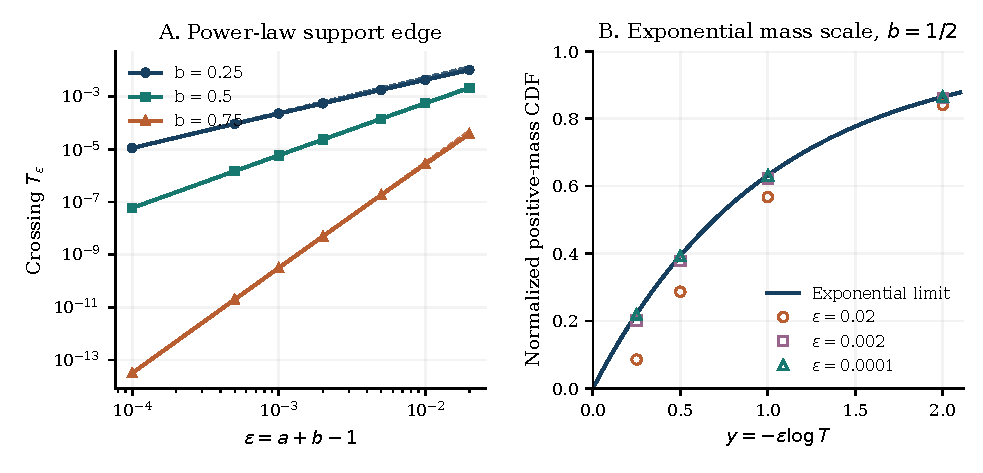
\includegraphics[width=\textwidth]{figures/real_boundary_two_scales.pdf}
\caption{The two scales of endpoint concentration. Left: numerical
crossings (markers) and the leading power laws (dashed curves) at three
fixed inner orders. Right: four sampled distribution-function values
for each indicated $\varepsilon$ at $b=1/2$, compared with the proved
unit-exponential limit. These are diagnostics of the analytic results.}
\label{rwbound:real:fig:boundary}
\end{figure}

All limits in this section keep $b$ fixed. As $b\downarrow0$, the
small parameter $\tau_\varepsilon/\varepsilon$ has exponent
$b/(1-b)\downarrow0$, so the stated hierarchy is not uniform at that
endpoint. As $b\uparrow1$, the exponent $1/(1-b)$ and the constants
become singular. Joint limits involving either endpoint require
additional analysis and are not consequences of these theorems.

\section{Euler enclosures and the failure of an unrestricted constant one}
\label{rw:sec:euler}

Let $a,b>0$ with $w\ge1$. Define
\begin{equation}\label{rw:eq:eulerdef}
 f(n)=c_{2n+1}=\frac{H_{2n}^{(b)}}{(2n+1)^a},\qquad
 d_k=\sum_{n=0}^k(-1)^n\binom kn f(n),\qquad
 E_N=\sum_{k=0}^{N-1}\frac{d_k}{2^{k+1}}.
\end{equation}
The error is measured against $g_{a,b}=\Imag F_{a,b}(\iu)$.
On the critical line this is an Abel value; the ordinary alternating
series with terms $(-1)^nf(n)$ diverges by the term test.

\begin{theorem}[Extended one-sided Euler bounds]\label{rw:thm:euler}
For every $k\ge1$ one has $d_k<0$, while $d_0=0$. The $E_N$ decrease
strictly to $g_{a,b}$, and
\begin{equation}\label{rw:eq:exacteuler}
 E_N-g_{a,b}=-2^{-N}\int_{[0,1]}
       \frac{(1-u^2)^N}{1+u^2}\dd\nu_{a,b}(u)>0.
\end{equation}
Consequently
\begin{equation}\label{rw:eq:eulerenclosure}
 E_N-M(a,b)2^{-N}<g_{a,b}<E_N\qquad(N\ge1),
\end{equation}
with the following elementary choices:
\begin{equation}\label{rw:eq:Mchoices}
 M(a,b)=
 \begin{cases}
 1,&a\ge1,\\
 (1-b)^{-1},&0<a<1,\ 0<b<1,\ w\ge1,\\
 b/(b-1),&0<a<1,\ b>1,\\
 1+1/a,&0<a<1,\ b=1.
 \end{cases}
\end{equation}
On the critical line the sharper uniform choice is proved in
Corollary~\ref{subpick:cor:sharp-critical}; its matching subcritical
Euler theorem uses the positive difference measure.
The choice one in the first line is the prior optimal universal
constant on that restricted domain; it is not asserted to work in
the other lines.
\end{theorem}
\begin{proof}
The binomial theorem and \eqref{subunit:eq:moments} give
$d_k=\int(1-u^2)^k\dd\nu(u)$. Thus $d_0=0$, while the strictly
decreasing weight gives $d_k<0$ for $k\ge1$. With
$m=m(\nu)$, we have $|d_k|\le m$. Therefore the Euler series is
absolutely convergent and may be summed under the measure integral:
\[
 \sum_{k\ge0}\frac{d_k}{2^{k+1}}
 =\int\frac{\dd\nu(u)}{1+u^2}=\Imag F(\iu).
\]
Summing the geometric tail gives \eqref{rw:eq:exacteuler}. Its weight
is strictly decreasing, bounded by one, and strictly less than one
for every $u>0$. Since the negative Jordan part has no atom at zero,
$0<E_N-g<m2^{-N}$. It remains to bound $m$.

For $b<1,w>1$, rewrite \eqref{subunit:eq:generalK} as
\[
 K_{a,b}=\frac{k_{w-1}}{1-b}
          -\bigl[-\zeta(b)k_a+C_{a,b}\bigr].
\]
The two displayed densities are positive, and each has mass
$1/(1-b)$ in the $u$ measure, by zero total mass. Hence
$m<1/(1-b)$. On $w=1$ the exact Jordan mass is $1/a=1/(1-b)$.
For $b>1$, \eqref{subunit:eq:generalK} is a difference of positive densities
$\zeta(b)k_a$ and $k_{w-1}/(b-1)+C_{a,b}$, so
$m<\zeta(b)<1+1/(b-1)=b/(b-1)$.

For $b=1$ and $0<a<1$, use a translation estimate rather than the
singular limit of either of these bounds. Let $\sigma_a$ be the
probability law of $u=e^{-Y}$ with $Y\sim\mathrm{Gamma}(a,1)$.
Its logarithmic density $p_a(s)=e^{-s}s^{a-1}/\Gamma(a)$ decreases
strictly. If $D_{e^{-t}}$ denotes pushforward under $u\mapsto e^{-t}u$,
then direct comparison of $p_a(s)$ and $p_a(s-t)$ gives
\[
 \|\sigma_a-D_{e^{-t}}\sigma_a\|_{\mathrm{TV}}
 =2\int_0^tp_a(s)\dd s
 \le\frac{2t^a}{\Gamma(a+1)}.
\]
The signed-measure integral
\[
 \widetilde\nu=\int_0^\infty
       \frac{\sigma_a-D_{e^{-t}}\sigma_a}{e^t-1}\dd t
\]
converges in total variation. Its $(n-1)$st moment is
$n^{-a}\int_0^\infty(1-e^{-(n-1)t})(e^t-1)^{-1}\dd t=c_n$.
By uniqueness it is $\nu_{a,1}$, and
\[
 m\le\frac1{\Gamma(a+1)}\int_0^\infty\frac{t^a}{e^t-1}\dd t
 =\zeta(a+1)<1+1/a.
\]

Finally, for $a\ge1$ the earlier sharper bound can be recovered
without any fractional-order gap. At $a=1$ the equivalent base density is
\[
 K_{1,b}(T)=-\frac{T^b}{\Gamma(b+1)}
 +\frac1{\Gamma(b)}\int_T^\infty\frac{t^{b-1}}{e^t-1}\dd t.
\]
Its $n$th Laplace value is
$-n^{-b-1}+n^{-1}\sum_{j=1}^n j^{-b}=H_{n-1}^{(b)}/n$,
by Tonelli and a finite geometric sum. Moment uniqueness therefore
identifies this base density with \eqref{subunit:eq:generalK} or \eqref{subunit:eq:bOne}.
Both positive terms in this difference have $e^{-T}\dd T$ integral
one. For the second term, interchange the integrals and use
$(1-e^{-t})/(e^t-1)=e^{-t}$; the first is a gamma integral.
Their positive overlap makes the Jordan mass strictly less than one.
For $a>1$, convolution by $k_{a-1}$ in the $T$ coordinate preserves
moments after multiplication by $n^{-(a-1)}$ and contracts the
$L^1(e^{-T}\dd T)$ norm, because
$\int_0^\infty e^{-T}k_{a-1}(T)\dd T=1$.
Moment uniqueness identifies the result with the present kernel,
so $m<1$ for every real $a\ge1$. This proves all four choices.
\end{proof}

The same translation proof gives, when $0<a\le1$ and $a+b>1$,
the optional non-elementary bound
\[
 m\le\frac{\Gamma(a+b)\zeta(a+b)}{\Gamma(a+1)\Gamma(b)}.
\]
It may improve a particular estimate, but diverges as $a+b\downarrow1$.
The critical atomic construction is therefore not replaced by this
translation argument.

\begin{proposition}[Exact finite Euler weights]\label{rw:prop:weights}
For $N\ge1$,
\begin{equation}\label{rw:eq:weights}
 E_N=2^{-N}\sum_{n=0}^{N-1}(-1)^nf(n)
                  \sum_{j=n+1}^N\binom Nj.
\end{equation}
Thus the finite sum can be formed without constructing a triangular
difference table.
\end{proposition}
\begin{proof}
Substitute the definition of $d_k$ and interchange the finite sums.
The coefficient identity is
\[
 \sum_{k=n}^{N-1}2^{N-k-1}\binom kn=\sum_{j=n+1}^N\binom Nj,
\]
which follows by induction from Pascal's identity. Harmonic numbers
and binomial tails can then each be updated successively. This
rearrangement is already used in the integer-order manuscript; the
new feature in the implementation here is certified rational
interval arithmetic for fractional powers.
\end{proof}

\begin{theorem}[A certified scope obstruction]\label{rw:thm:counterexample}
For $a=1/10$ and $b=9/10$,
\begin{align}\label{rw:eq:counterinterval}
 -0.5297619322857712630946293655
 &<g_{1/10,9/10}\notag\\
 &<-0.5297619322857712630946293653.
\end{align}
In particular, $g_{1/10,9/10}<-13/25<-1/2$.
Since $E_1=0$, the inequality $E_N-2^{-N}<g_{a,b}$ fails at $N=1$
for this pair. A uniform constant one cannot be extended to the
entire region $a+b\ge1$. The failure also occurs strictly above
the threshold, with ordinary boundary convergence:
\begin{align}\label{rw:eq:counterordinary}
 -0.5308442529661593261720712602
 &<g_{1/10,1}\notag\\
 &<-0.5308442529661593261720712600<-0.53.
\end{align}
\end{theorem}
\begin{proof}
The accompanying standard-library program \texttt{code/certify.py}
evaluates \eqref{rw:eq:weights} with $N=96$ by outward rational interval
arithmetic. Every fractional power is bounded by integer tenth-root
inequalities, as detailed in Section~\ref{rw:sec:certificates}. The
critical mass bound is the exact rational $M=10$. Subtracting
$10\,2^{-96}$ from the lower endpoint of the finite Euler enclosure
and leaving its upper endpoint unchanged gives the interval recorded
in \texttt{data/exact\_certificates.json}. Outward decimal rounding
yields \eqref{rw:eq:counterinterval}; exact rational comparisons verify
its upper endpoint is less than $-13/25$. No numerical polylogarithm,
floating-point root, or unproved identity enters this certificate.
For $(a,b)=(1/10,1)$ the same computation uses $M=1+1/a=11$
and proves \eqref{rw:eq:counterordinary}. Its ordinary boundary
convergence follows from $a+b=11/10>1$ and
Corollary~\ref{rw:cor:boundary}.
\end{proof}

This is \emph{not} a counterexample to the baseline theorem, which
explicitly assumes $a\ge1$. It is a counterexample to dropping that
hypothesis while retaining the same universal error constant.

\begin{proposition}[The exact critical constant for fixed parameters]
\label{rw:prop:fixedconstant}
On $a+b=1$, put $d\sigma=-K_{1-b,b}(-\log u)\,du$. The scaled errors $2^N(E_N-g_{a,b})$ decrease strictly
to zero for $N\ge1$. The smallest constant in the non-strict estimate
$E_N-g_{a,b}\le C2^{-N}$, valid for all integers $N\ge1$ at that fixed
pair, is $C=-2g_{a,b}$.
\end{proposition}
\begin{proof}
The endpoint atom contributes zero to \eqref{rw:eq:exacteuler} when
$N\ge1$. Hence
\[
 2^N(E_N-g)=\int_0^1\frac{(1-u^2)^N}{1+u^2}\dd\sigma(u).
\]
Strict pointwise decrease and dominated convergence prove the first
claim. Its largest value occurs at $N=1$ and is $2(E_1-g)=-2g$.
For the corresponding strict inequality the infimum of admissible
constants is the same, but equality at $N=1$ prevents attaining it.
\end{proof}


\subsection{Exact arithmetic and independent native evidence}
\label{rw:sec:certificates}
The new standard-library verifier encloses every rational fractional power
by integer root inequalities on a $10^{100}$ grid. Products, harmonic sums
and finite Euler weights are then combined as exact rational intervals.
It certifies 616 strictly positive Hausdorff-difference signs, 112 negative
Euler increments and seven Gaussian analytic-value enclosures at 192
Euler terms. The six triangle cases use the rational budget $57/50$;
the remaining axis case uses $5/4$. The axis case $b=3/2$ also proves
$-2g_{0,3/2}>227/200$, supplying the finite arithmetic premise in the
axis-maximum theorem.

A separate native Wolfram calculation at 100 working digits evaluates
the outer Gamma integral of a depth-one polylogarithm, or the direct
axis value. All seven values lie inside their rational Euler enclosures.
The native quadrature is a numerical diagnostic, not interval quadrature.
The sign and remainder theorems depend on the written positive-measure
proofs. The original threshold report's tenth-root certificates are
preserved unchanged with its delivered code and data.

\section{A sharp Euler constant at every positive real order}
\label{univeuler:sec:main}
The Gaussian maximum does not bound arbitrary Euler errors merely because
it bounds the value of the function. A contraction inequality for the
Euler kernel supplies the missing implication. It removes the divergent
parameter-dependent budgets near the signed-measure threshold, while
retaining the stronger constant one on the earlier domain $a\ge1$.

\begin{lemma}[A difference-of-powers bound]\label{univeuler:lem:powers}
For $m\ge2$, $0\le r\le1$ and $0\le v\le1$,
\[
 0\le(1-rv)^m-(1-r)^m\le\frac{1-v}{1+v}.
\]
For $0<v<1$, equality on the right is possible only when $m=2$,
and then it holds precisely at $r=1/(1+v)$.
\end{lemma}
\begin{proof}
The endpoints $v=0,1$ are immediate. Fix $0<v<1$ and put
$q=v^{1/(m-1)}$. Differentiation shows that the unique maximum over
$r\in[0,1]$ is at $r=(1-q)/(1-vq)$, where its value is
\[
 \frac{(1-v)^m}{(1-v^{m/(m-1)})^{m-1}}.
\]
Let $p=m/(m-1)\in(1,2]$. The function
$p\mapsto\log(1-v^p)$ has strictly negative second derivative
$-(\log v)^2v^p/(1-v^p)^2$. Its chord between $p=1$ and $p=2$
therefore gives
\[
 1-v^p\ge(1-v)(1+v)^{p-1},
\]
strictly when $1<p<2$. Substitution in the maximum proves the bound
and both equality assertions.
\end{proof}

\begin{lemma}[Contraction of the Euler tail kernel]
\label{univeuler:lem:contraction}
For an integer $N\ge1$, set $H_N(t)=(1-t)^N/(1+t)$ on $[0,1]$.
For $0\le r,v\le1$,
\begin{equation}\label{univeuler:eq:contraction}
 0\le H_N(rv)-H_N(r)\le\frac{1-v}{1+v}.
\end{equation}
If $0<v<1$, equality on the right holds precisely when $N=1$ and $r=1$.
\end{lemma}
\begin{proof}
For $N=1$, the difference between the right side and the middle
expression factors exactly as
\[
 \frac{(1-v)(1-r)(1-rv)}{(1+v)(1+rv)(1+r)}.
\]
For $N\ge2$, the uniformly convergent positive expansion
\[
 H_N(t)=\sum_{k\ge0}\frac{(1-t)^{N+k}}{2^{k+1}}
\]
expresses its difference as a probability-weighted sum of the preceding
power differences. Each is bounded as claimed, and the terms with
$N+k>2$ make the upper inequality strict for $0<v<1$. Decrease of
$H_N$ proves the lower inequality.
\end{proof}

Let $\omega_b$ be the probability measure
\[
 d\omega_b(v)=\frac{(-\log v)^{b-1}}{\Gamma(b)}\,dv,
 \qquad 0<v<1.
\]
Let $\pi_a$ be the law of $X=e^{-T_a}$ with
$T_a\sim\mathrm{Gamma}(a,1)$ when $a>0$, and put $\pi_0=\delta_1$.
These measures are independent. They retain ordinary probability mass
throughout the parameter domain, including the critical and subcritical
regions where the unweighted one-variable moment measure is not finite.

\begin{theorem}[All-order Euler representation and the sharp universal constant]
\label{univeuler:thm:sharp}
For every $a\ge0,b>0$, define $d_k$ and $E_N$ from the coefficients
$c_{2n+1}$ as in \eqref{rw:eq:eulerdef}, and use the analytic value
$g_{a,b}=\Imag F_{a,b}(i)$. Then $d_0=0$, $d_k<0$ for $k\ge1$,
and $E_N$ decreases strictly to $g_{a,b}$. Its exact error is
\begin{equation}\label{univeuler:eq:tail}
 2^N(E_N-g_{a,b})=
 \int\!\!\int
 \frac{H_N(x^2v^2)-H_N(x^2)}{1-v}\,d\pi_a(x)\,d\omega_b(v).
\end{equation}
Consequently, for every $N\ge1$,
\begin{equation}\label{univeuler:eq:axisbudget}
 0<2^N(E_N-g_{a,b})\le C(b),\qquad
 C(b)=\beta(b)+2^{-b}\eta(b).
\end{equation}
Equality in the upper bound holds exactly when $a=0$ and $N=1$.
The sharp uniform constant over all nonnegative outer orders is
\[
 C_* = C(b_*),
\]
where $b_*$ is the unique nondegenerate maximum from
Theorem~\ref{subpick:thm:axis-maximum}. It satisfies
\[
 \frac{227}{200}<C_*<\frac{1+\sqrt2}{2}<\frac54.
\]
For positive $a,b$ the strict inequality
$0<E_N-g_{a,b}<C_*2^{-N}$ holds, and $C_*$ is its least possible
uniform constant. When $a=0$ is included, the non-strict upper bound
is attained only at $a=0,b=b_*,N=1$.
\end{theorem}
\begin{proof}
The elementary moment laws give, for $n\ge0$,
\[
 c_{2n+1}=\int\!\!\int x^{2n}
             \frac{1-v^{2n}}{1-v}\,d\pi_a(x)\,d\omega_b(v).
\]
Indeed the two factors integrate to $(2n+1)^{-a}$ and $H_{2n}^{(b)}$.
The quotient is a finite geometric sum, so this identity includes $n=0$
without an endpoint singularity. Finite binomial expansion now gives
\[
 d_k=\int\!\!\int
       \frac{(1-x^2)^k-(1-x^2v^2)^k}{1-v}
                 \,d\pi_a(x)\,d\omega_b(v).
\]
For $k\ge1$ its integrand is strictly negative and has absolute value
at most $2k$, by the mean-value theorem. Finite summation is therefore
legitimate for every pair of parameters.

The Gaussian double kernel, or the axis formula when $a=0$, gives
\[
 g_{a,b}=\int\!\!\int
 \frac{(1+x^2)^{-1}-(1+x^2v^2)^{-1}}{1-v}
                    \,d\pi_a(x)\,d\omega_b(v).
\]
Its integrand is $-x^2(1+v)/((1+x^2)(1+x^2v^2))$, hence bounded.
Subtract the finite geometric sum defining $E_N$ from this identity
to obtain \eqref{univeuler:eq:tail}; no divergent boundary series is used.

Apply Lemma~\ref{univeuler:lem:contraction} with $r=x^2$ and its
variable $v$ replaced by $v^2$. The resulting majorant is
\[
 \frac{1-v^2}{(1-v)(1+v^2)}=\frac{1+v}{1+v^2}.
\]
Its $\omega_b$ integral is $C(b)$ by the axis identity.
It is bounded by $(1+\sqrt2)/2$, so the exact error tends to zero
at least geometrically. The strict signs of $d_k$ give the strict
decrease of $E_N$. The contraction equality criterion and the positive
densities of both probability measures prove the fixed-$b$ equality claim.

The unique axis maximum supplies the uniform constant and its bounds.
Sharpness over $a,b>0$ follows by fixing $b=b_*$, taking $a\downarrow0$
at $N=1$, and using bounded convergence in the Gaussian probability
integral. Thus the supremum is approached at the axis, while inclusion
of the axis gives the stated unique attaining triple.
\end{proof}

This theorem closes the previously open universal real-order Euler-budget
question. The separate contraction argument is essential: Gaussian
magnitude alone would not control later scaled errors. In particular,
this result does not say that their maximum at each positive parameter
pair is the first error, nor that the scaled errors always decrease.
The constant one remains sharper on $a\ge1$, and the sharp critical
constant $\pi/4+\log2/2$ remains sharper on $a+b\le1$.
The decimal diagnostic $C_*\approx1.13656110333950956095$ inherits the
axis experiment's status; the exact definition and inequalities above
are proved without relying on those digits.

\section{A uniform rational kernel inequality}
\label{latebudget:sec:ineq}
The independent continuations~\cite{latebudget:sharp,latebudget:golden}
separate the first Euler step from every later one. Retain the residual
function $H_N(t)$ above, and define the continuously extended kernel
\[
 K_N(p,y)=\frac{H_N(py^2)-H_N(p)}{1-y},\qquad
 K_N(p,1)=-2pH_N'(p).
\]
It is nonnegative. The following finite polynomial certificate and analytic
mixture reduction prove a stronger uniform budget for $N\ge2$.

\begin{theorem}[Kernel bound for every later truncation]\label{latebudget:thm:kernel}
For every integer $N\ge2$ and $0\le p,y\le1$,
\begin{equation}\label{latebudget:eq:kernel-bound}
 0\le K_N(p,y)<\frac98.
\end{equation}
The lower bound is strict when $p>0$ and $y<1$. The strict upper bound includes the continuous boundary values.
\end{theorem}
The proof has two finite base cases and an all-$N$ envelope. We give enough information to reconstruct every rational certificate without a symbolic algebra system.

\subsection{Two explicit polynomial base cases}
Multiplication by the positive denominator shows that $K_N<9/8$ is equivalent to positivity of
\[
 P_N(p,y)=8(1+p)(1+py^2)\{9/8-K_N(p,y)\}.
\]
For $N=2,3$ these are the following polynomials:
\begin{align}
P_2={}&8y^2(1+y)p^3+(8y^3+17y^2+8y+8)p^2\notag\\
&+(9y^2-24y-15)p+9,\label{latebudget:eq:P2}\\
P_3={}&-8y^2(y+1)(y^2+1)p^4\notag\\
&+(-8y^5-8y^4+16y^3+16y^2-8y-8)p^3\notag\\
&+(24y^3+33y^2+24y+24)p^2
 +(9y^2-32y-23)p+9.\label{latebudget:eq:P3}
\end{align}
An identity check can avoid rational-function division altogether:
\begin{align}\label{latebudget:eq:polynomial-check}
(1-y)P_N={}&9(1-y)(1+p)(1+py^2)\notag\\
&-8\{(1-py^2)^N(1+p)-(1-p)^N(1+py^2)\}.
\end{align}
Both verifiers check this identity or independently reconstruct its quotient.

For a polynomial $P(x,y)=\sum c_{kl}x^ky^l$ of bidegree at most $(r,s)$, its tensor Bernstein coefficients on the unit square are
\begin{equation}\label{latebudget:eq:bernstein}
 B_{ij}=\sum_{k\le i,\,l\le j}c_{kl}
 \frac{\binom ik}{\binom rk}\frac{\binom jl}{\binom sl}.
\end{equation}
The Bernstein basis functions are nonnegative and sum to one. Hence a strictly positive minimum of these coefficients proves strict positivity of $P$ on the whole square, including its boundary.

For a mesh of denominator $d$, first substitute
$p=(u+i)/d$, $y=(v+j)/d$ on each cell. Formula \eqref{latebudget:eq:bernstein} then gives an exact certificate. The data are summarized by
\begin{center}
\begin{tabular}{lrrrr}
\toprule
Polynomial & Bidegree & Mesh & Coefficients & Smallest coefficient\\
\midrule
$P_2$ & $(3,3)$ & $8\times8$ & $1024$ & $631/12288$\\
$P_3$ & $(4,5)$ & $4\times4$ & $480$ & $11337/40960$\\
\bottomrule
\end{tabular}
\end{center}
Every coefficient is stored as a rational number in the accompanying JSON file. More importantly, the standard-library verifier regenerates all of them from \eqref{latebudget:eq:P2}--\eqref{latebudget:eq:bernstein}; it does not trust a stored minimum. These finitely many exact additions and multiplications prove the two base cases.

\subsection{An envelope for binomial differences}
Introduce
\[
 J_m(p,y)=\frac{(1-py^2)^m-(1-p)^m}{1-y},\qquad m\ge2.
\]
For fixed $0<y<1$, differentiation in $p$ gives a unique interior maximum at
\begin{equation}\label{latebudget:eq:pmax}
 p_m(y)=\frac{1-y^{2/(m-1)}}{1-y^{2m/(m-1)}}.
\end{equation}
Indeed the derivative changes sign exactly when
$1-p=y^{2/(m-1)}(1-py^2)$. Its sign is positive at $p=0$ and negative at $p=1$. Substitution yields the exact envelope
\begin{equation}\label{latebudget:eq:envelope}
 J_m(p,y)\le B_m(y):=(1+y)
 \left(\frac{1-y^2}{1-y^{2m/(m-1)}}\right)^{m-1}.
\end{equation}
The endpoint values follow by continuity.

\begin{lemma}[The binomial envelope decreases in its index]\label{latebudget:lem:envelope}
For every $0<y<1$, $B_{m+1}(y)<B_m(y)$ for $m\ge2$.
\end{lemma}
\begin{proof}
Put $k=m-1$, $t=-2\log y>0$ and
$h(v)=\log(1-e^{-(1+v)t})$. Direct differentiation gives $h''(v)<0$ for $v\ge0$. Apart from $\log(1+y)$, the logarithm of \eqref{latebudget:eq:envelope} is
\[
 k\{h(0)-h(1/k)\}=-\frac{h(1/k)-h(0)}{1/k}.
\]
The secant slope of a strictly concave function decreases as the right endpoint increases. Thus the displayed negative secant slope decreases strictly when $k$ increases. Exponentiation proves the claim.
\end{proof}

\subsection{The fourth envelope is below nine eighths}
Set $y=t^3$, $0\le t\le1$. The inequality $B_4(y)<9/8$ is equivalent away from $t=1$ to
\begin{equation}\label{latebudget:eq:Qfactor}
9(1-t^8)^3-8(1+t^3)(1-t^6)^3=(1-t^2)^3Q(t)>0,
\end{equation}
where
\begin{align}\label{latebudget:eq:Q}
Q(t)={}&9t^{18}+27t^{16}-8t^{15}+54t^{14}-24t^{13}+82t^{12}
 -48t^{11}\notag\\
&+84t^{10}-56t^9+60t^8-48t^7+34t^6-24t^5
 +6t^4-8t^3+3t^2+1.
\end{align}
The degree-18 Bernstein coefficients after $t=u/2$ and $t=(1+u)/2$ have respectively the strictly positive minima
\begin{equation}\label{latebudget:eq:Qmin}
 \frac{192789}{262144},\qquad \frac{690189}{1949696}.
\end{equation}
There are only $38$ coefficients. Formula \eqref{latebudget:eq:bernstein} with one variable regenerates them. At $y=1$ the envelope limit is
$B_4(1)=2(3/4)^3=27/32<9/8$, so the endpoint is covered as well.

\subsection{The infinite family follows without an infinite computation}
Since $1/(1+v)=\sum_{j\ge0}(1-v)^j/2^{j+1}$ on $[0,1]$,
\begin{equation}\label{latebudget:eq:mixture}
 K_N(p,y)=\sum_{j=0}^{\infty}2^{-j-1}J_{N+j}(p,y).
\end{equation}
For $y<1$ this follows by subtracting the two convergent geometric series. If $N\ge4$, \eqref{latebudget:eq:envelope}, Lemma~\ref{latebudget:lem:envelope} and \eqref{latebudget:eq:Qfactor} give
\[
 J_{N+j}(p,y)\le B_{N+j}(y)\le B_4(y)<9/8.
\]
Averaging proves $K_N\le B_4<9/8$ for every $N\ge4$. Continuity covers $y=1$. The polynomial base cases cover $N=2,3$, completing Theorem~\ref{latebudget:thm:kernel}.


\begin{corollary}[A smaller uniform budget after the first step]
\label{latebudget:cor:error}
For every $a\ge0,b>0$ and integer $N\ge2$,
\[
 0<2^N(E_N-g_{a,b})<\frac98.
\]
\end{corollary}
\begin{proof}
Take expectations of the strict pointwise inequality in
\eqref{univeuler:eq:tail}, with $p=x^2$ and $y=v$.
The measures are probability measures, and their kernel is strictly
positive almost everywhere, including the $a=0$ axis.
\end{proof}
The first-step maximum $C_*$ is strictly larger than $9/8$, already by
$C_*>227/200$ in Theorem~\ref{univeuler:thm:sharp}. This does not imply
that scaled errors decrease at each fixed pair: the exact incoming replay
certifies $R_2(4,1)>R_1(4,1)$, where $R_N=2^N(E_N-g)$.
The unscaled $E_N$ still decrease by the theorem above.


\begin{remark}[Nature of the finite computation]
The inequality is a computer-assisted ordinary proof: three stated polynomial identities, a stated rational basis conversion, and $1542$ strictly positive rational numbers close its finite component. The all-index reduction is analytic. The check is reproducible under Python's optimized mode and is not a test of finitely many real sample points. The supplied SymPy replay independently derives the two rational kernels rather than importing their coefficient arrays.
\end{remark}

The fresh standard-library replay regenerates all 1,542 coefficients on
82 cells, checks the three defining polynomial identities, and rejects a
corrupted polynomial. The same verifier succeeds with optimized Python,
whose disabled assertions do not bypass its explicit validations. A
separate SymPy program reconstructs the base rational kernels. Receipts
are preserved in \src{verification/sixth-replay/sharp/}. The independently
replayed golden/Cayley delivery uses another positive-mixture route and
its own finite base certificates; it is supporting evidence for the same
bound, not a second definition of the sharp all-index constant.


\section{A geometric evaluation formula that survives \texorpdfstring{$xy=1$}{xy=1}}
\label{cert:sec:spectral}
The preceding sections concern finite identities. We now give an evaluation
method for the full double polylogarithm, including components for which
no finite classical reduction has been established.

\begin{lemma}[One-dimensional integral]
\label{cert:lem:integral}
For $a,b\ge1$, $|x|\le1$, $x\ne1$, and $|y|\le1$,
\begin{equation}
 \Li_{a,b}(x,y)=\frac{x}{(a-1)!}
  \int_0^1\frac{(-\log t)^{a-1}\Li_b(xyt)}{1-xt}\,dt.
\label{cert:eq:integral}
\end{equation}
\end{lemma}
\begin{proof}
For $|x|<1$, the Mellin identity
$n^{-a}=\int_0^1 t^{n-1}(-\log t)^{a-1}\,dt/(a-1)!$
and absolute convergence give
\[
 \sum_{n>m\ge1}(xt)^ny^m/m^b
 =\frac{xt}{1-xt}\Li_b(xyt).
\]
This proves \eqref{cert:eq:integral}. For a nontrivial unit outer argument,
$1-rxt$ stays uniformly away from zero for $r$ sufficiently close to one.
Also $|\Li_b(rxyt)|\le\Li_b(t)$, and
\begin{equation}
 \frac1{(a-1)!}\int_0^1(-\log t)^{a-1}\Li_b(t)\,dt
 =\sum_{m\ge1}\frac1{m^b(m+1)^a}\le\zeta(a+b).
\label{cert:eq:momentbound}
\end{equation}
Dominated convergence and summation by parts in the nested series therefore give the boundary
case. Notice that $xy=1$ causes no problem: the logarithmic endpoint at
$b=1$ is integrable in \eqref{cert:eq:momentbound}.
\end{proof}

Let $T_n$ denote the Chebyshev polynomial defined by
$T_n(\cos u)=\cos(nu)$. Put
\begin{equation}
 d=\sqrt{1-x},\qquad r=\frac{1-d}{1+d},\qquad R=|r|,
\label{cert:eq:dr}
\end{equation}
where the square root has positive real part. For $|x|\le1$, $x\ne1$,
we have $\Real d>0$ and therefore $R<1$.

\begin{lemma}[The kernel expansion]
\label{cert:lem:kernel}
Uniformly for $0\le t\le1$,
\begin{equation}
 \frac1{1-xt}=\frac1d\left(1+2\sum_{n\ge1}r^nT_n(2t-1)\right).
\label{cert:eq:kernel}
\end{equation}
\end{lemma}
\begin{proof}
For $s\in[-1,1]$, summing the two geometric series associated with
$s=\cos u$ gives the classical identity
\[
 1+2\sum_{n\ge1}r^nT_n(s)=\frac{1-r^2}{1-2rs+r^2}.
\]
This is also a direct consequence of the generating function in
\cite{hstruct:DLMF}. Substituting \eqref{cert:eq:dr} shows
\[
 1-xt=d\frac{1-2r(2t-1)+r^2}{1-r^2}.
\]
The series is uniform because $|T_n(s)|\le1$ and $R<1$.
\end{proof}

\begin{definition}
For $v=xy$ and $n\ge0$, define the Chebyshev moment
\begin{equation}
 \mathcal M_n^{a,b}(v)=\frac1{(a-1)!}
 \int_0^1(-\log t)^{a-1}T_n(2t-1)\Li_b(vt)\,dt.
\label{cert:eq:Chebmoment}
\end{equation}
\end{definition}

\begin{theorem}[Certified Chebyshev--moment expansion]
\label{cert:thm:spectral}
Under the hypotheses of Lemma~\ref{cert:lem:integral}, with $x\ne0$,
\begin{equation}
 \Li_{a,b}(x,y)=\frac{x}{d}
 \left(\mathcal M_0^{a,b}(v)+2\sum_{n\ge1}r^n\mathcal M_n^{a,b}(v)\right).
\label{cert:eq:spectral}
\end{equation}
For $K\ge1$, let $E_K$ be the difference between the left side and the
truncation with indices $0\le n<K$. Then
\begin{equation}
 |E_K|\le
 \frac{2|x|\zeta(a+b)}{|d|(1-R)}R^K.
\label{cert:eq:error}
\end{equation}
This estimate is uniform over $|y|\le1$, including $xy=1$.
For nontrivial level-three or level-four outer roots,
\begin{equation}
 |E_K|\le\frac{16}{3\,4^K}.
\label{cert:eq:uniformerror}
\end{equation}
\end{theorem}
\begin{proof}
Insert \eqref{cert:eq:kernel} into \eqref{cert:eq:integral}. The integrable majorant
in \eqref{cert:eq:momentbound} justifies termwise integration and gives
$|\mathcal M_n^{a,b}(v)|\le\zeta(a+b)$ for all $n$.
The tail of the resulting geometric series is \eqref{cert:eq:error}.
For the specified roots, direct substitution in \eqref{cert:eq:dr} gives
$R<1/4$ and $|d|>1$; the code also proves these inequalities by interval
arithmetic before using them. Since $\zeta(a+b)\le\zeta(2)<2$, the
bound becomes $4(1/4)^K/(1-1/4)=16/(3\,4^K)$.
The zero outer argument, omitted only to avoid unnecessary notation,
gives $\Li_{a,b}(0,y)=0$ directly.
\end{proof}

The proof does not appeal to cancellation in a sampled sequence, a fitted
asymptotic expansion, or an empirical convergence diagnostic. In particular,
when the product of two roots is one, the same argument and the same bound
apply. The only new feature is the elementary cancellation in the exact
moment formula, to which we now turn.

\section{Every moment reduces to classical polylogarithms}
\label{cert:sec:moments}
Write the shifted Chebyshev polynomial as
\begin{equation}
 Q_n(t):=T_n(2t-1)=\sum_{j=0}^n c_{n,j}t^j.
\label{cert:eq:Q}
\end{equation}
Its coefficients are integers and can be generated without symbolic
integration:
\begin{equation}
 Q_0=1,\quad Q_1=2t-1,\quad Q_{n+1}=2(2t-1)Q_n-Q_{n-1}.
\label{cert:eq:Qrec}
\end{equation}
Thus
\begin{equation}
 \mathcal M_n^{a,b}(v)=\sum_{j=0}^n c_{n,j}J_{a,b}(j+1;v),
\label{cert:eq:momentpoly}
\end{equation}
where
\begin{equation}
 J_{a,b}(c;v)=\sum_{m\ge1}\frac{v^m}{m^b(m+c)^a},\qquad c\in\Z_{>0}.
\label{cert:eq:J}
\end{equation}
The power series in \eqref{cert:eq:J} is absolutely convergent for $|v|\le1$.

\begin{lemma}[Two-pole partial fractions]
\label{cert:lem:partial}
Put
\begin{align}
 A_s&=(-1)^{b-s}\binom{a+b-s-1}{a-1}c^{-(a+b-s)}
          &&(1\le s\le b),\notag\\
 C_s&=(-1)^b\binom{a+b-s-1}{b-1}c^{-(a+b-s)}
          &&(1\le s\le a).
\label{cert:eq:AC}
\end{align}
Then, for $u\ne0,-c$,
\begin{equation}
 \frac1{u^b(u+c)^a}=\sum_{s=1}^b\frac{A_s}{u^s}
                          +\sum_{s=1}^a\frac{C_s}{(u+c)^s}.
\label{cert:eq:partial}
\end{equation}
In particular, $A_1+C_1=0$.
\end{lemma}
\begin{proof}
The principal part at $u=0$ follows by expanding
$(u+c)^{-a}=c^{-a}(1+u/c)^{-a}$. Its coefficient of $u^{-s}$ after
multiplication by $u^{-b}$ is exactly $A_s$.
At $u=-c$, write $w=u+c$ and expand
$u^{-b}=(-1)^bc^{-b}(1-w/c)^{-b}$; this gives $C_s$.
The difference between the two sides has no finite poles and tends to
zero at infinity, so it is identically zero.
The equality $A_1=-C_1$ follows from
$\binom{a+b-2}{a-1}=\binom{a+b-2}{b-1}$.
\end{proof}

For $s\ge1$, let
$H_c^{(s)}(v)=\sum_{k=1}^c v^k/k^s$ and $H_c^{(s)}=H_c^{(s)}(1)$.
A coefficient outside the ranges in \eqref{cert:eq:AC} is understood to be
zero in the following theorem.

\begin{theorem}[Finite classical moment formula]
\label{cert:thm:moments}
For $0<|v|\le1$, $v\ne1$,
\begin{equation}
 J_{a,b}(c;v)=\sum_{s=1}^b A_s\Li_s(v)
       +v^{-c}\sum_{s=1}^a C_s\bigl(\Li_s(v)-H_c^{(s)}(v)\bigr).
\label{cert:eq:momentfinite}
\end{equation}
At the resonant endpoint $v=1$ the finite expression is instead
\begin{equation}
 J_{a,b}(c;1)
 =-C_1H_c^{(1)}+
   \sum_{s=2}^{\max(a,b)}(A_s+C_s)\zeta(s)
   -\sum_{s=2}^a C_sH_c^{(s)}.
\label{cert:eq:momentone}
\end{equation}
No regularized zeta value is needed. At $v=0$, $J_{a,b}(c;0)=0$.
\end{theorem}
\begin{proof}
Multiply \eqref{cert:eq:partial} by $v^m$ and sum over $m\ge1$.
For $|v|<1$, all rearrangements are absolute, and
\[
 \sum_{m\ge1}\frac{v^m}{(m+c)^s}
 =v^{-c}\bigl(\Li_s(v)-H_c^{(s)}(v)\bigr).
\]
Radial limits give \eqref{cert:eq:momentfinite} at $|v|=1$, $v\ne1$.
At $v=1$, combine the two $s=1$ pieces at the level of partial sums:
\[
 A_1\sum_{m=1}^N\frac1m+C_1\sum_{m=1}^N\frac1{m+c}
 =-C_1H_c^{(1)}+C_1\sum_{m=N+1}^{N+c}\frac1m.
\]
The last term tends to zero. Every $s\ge2$ term converges separately,
which gives \eqref{cert:eq:momentone}.
\end{proof}

For example, when $a=b=1$, \eqref{cert:eq:momentone} reduces to
\begin{equation}
 J_{1,1}(c;1)=\frac{H_c}{c}.
\label{cert:eq:J11}
\end{equation}
Consequently the resonant depth-two function has the explicit expansion
\begin{equation}
 \Li_{1,1}(x,x^{-1})=
 \frac{x}{\sqrt{1-x}}\left[
 1+2\sum_{n\ge1}r^n\sum_{j=0}^n c_{n,j}\frac{H_{j+1}}{j+1}
 \right],
\label{cert:eq:resonant11}
\end{equation}
valid for a nontrivial unit outer argument. Its coefficients are rational.
The error after $K$ terms is bounded by \eqref{cert:eq:error}, and the uniform
level-three/four bound \eqref{cert:eq:uniformerror} applies.
This is an exact infinite identity for a conditionally
convergent depth-two case; it is not a finite rational expression in
classical constants.

\subsection{A resonant example beyond the first weight}
For $(a,b)=(2,1)$, the coefficients are
$A_1=c^{-2}$, $C_1=-c^{-2}$, and $C_2=-c^{-1}$, giving
\begin{equation}
 J_{2,1}(c;1)=\frac{H_c}{c^2}+\frac{H_c^{(2)}-\zeta(2)}{c}.
\label{cert:eq:J21}
\end{equation}
Substitution in \eqref{cert:eq:momentpoly} and \eqref{cert:eq:spectral} yields a
geometrically convergent formula for
$\Li_{2,1}(\rho,\rho^{-1})$, $\rho=e^{2\pi\iu/3}$,
whose coefficient data involve only rational numbers and $\zeta(2)$.
The location of the singular product $v=1$ has become an explicit,
finite harmonic-sum correction rather than a numerical failure mode.

\section{Optimal geometric rate and the conductor dependence}
\label{cert:sec:optimal}
The rate in Theorem~\ref{cert:thm:spectral} is not merely an artifact of an
arbitrary expansion point. It is the best exponential rate obtainable
by uniformly approximating its outer rational kernel with polynomials.
This statement concerns the kernel, not the minimal complexity of all
possible algorithms for evaluating a special value.

\begin{theorem}[Sharp exponential rate for polynomial kernels]
\label{cert:thm:optimal}
Fix $0<|x|\le1$, $x\ne1$, and let $d,r,R$ be as in \eqref{cert:eq:dr}.
For $K\ge1$, define
\[
 e_{K-1}(x)=\inf_{\deg p<K}\max_{0\le t\le1}
           \left|\frac1{1-xt}-p(t)\right|,
\]
where the infimum allows complex polynomial coefficients. Then
\begin{equation}
 \frac{R^K}{|d|}\le e_{K-1}(x)
       \le\frac{2R^K}{|d|(1-R)}.
\label{cert:eq:bestpoly}
\end{equation}
In particular,
$\lim_{K\to\infty}e_{K-1}(x)^{1/K}=R$.
\end{theorem}
\begin{proof}
The upper bound is the uniform tail bound in \eqref{cert:eq:kernel}.
For the lower bound, use the $K$th Chebyshev coefficient of
$f(s)=(1-x(s+1)/2)^{-1}$. By \eqref{cert:eq:kernel}, it is $2r^K/d$.
The corresponding coefficient of a polynomial of degree less than $K$
vanishes. For any continuous complex function $g$ on $[-1,1]$,
\[
 \left|\frac2\pi\int_0^\pi g(\cos u)\cos(Ku)\,du\right|
 \le2\|g\|_\infty.
\]
Apply this with $g=f-p$ to obtain
$2R^K/|d|\le2\|f-p\|_\infty$ and take the infimum.
Taking $K$th roots proves the final statement.
\end{proof}

\begin{corollary}[Adjacent roots]
\label{cert:cor:conductor}
For $x_q=e^{2\pi\iu/q}$, as $q\to\infty$,
\begin{equation}
 -\log R_q=2\sqrt{\frac\pi q}+O(q^{-3/2}).
\label{cert:eq:rateq}
\end{equation}
For fixed $a,b$, the bound \eqref{cert:eq:error} guarantees an absolute error
at most $10^{-P}$ using
\begin{equation}
 K=O\bigl(\sqrt q(P+\log q)\bigr)
\label{cert:eq:Kq}
\end{equation}
outer-kernel terms, uniformly in $|y|\le1$.
\end{corollary}
\begin{proof}
With $\theta=2\pi/q$,
$d=\sqrt{1-e^{\iu\theta}}
=e^{-\iu\pi/4}\sqrt\theta\,(1+O(\theta))$.
Hence
\[
 -\log|r|=\Real\left(\log(1+d)-\log(1-d)\right)
 =2\Real(d+d^3/3+\cdots)
 =\sqrt{2\theta}+O(\theta^{3/2}),
\]
which is \eqref{cert:eq:rateq}. Also $|d|\asymp q^{-1/2}$ and
$1-R\asymp q^{-1/2}$, so the prefactor in \eqref{cert:eq:error} is $O(q)$.
Solving the resulting geometric inequality gives \eqref{cert:eq:Kq}.
\end{proof}

For comparison, expansion around $t=1/2$ gives
\[
 \frac1{1-xt}=\frac1{1-x/2}
 \sum_{n\ge0}\left(\frac{x(t-1/2)}{1-x/2}\right)^n.
\]
At a unit outer argument its uniform ratio is
$R_{\mathrm{mid}}=1/|2-x|$. For $x=x_q$,
\begin{equation}
 -\log R_{\mathrm{mid}}
 =\tfrac12\log(5-4\cos(2\pi/q))
 =\frac{4\pi^2}{q^2}+O(q^{-4}).
\label{cert:eq:midrate}
\end{equation}
Thus its corresponding sufficient degree is
$O(q^2(P+\log q))$. This is a comparison between two proved expansions,
not a claim to improve every previously published polylogarithm algorithm.

\paragraph{Arithmetic cost versus approximation degree.}
With weights fixed, the monomial moments for $1\le c\le K$ can be
assembled from finitely many single values and incrementally updated
$H_c^{(s)}(v)$ in $O((a+b)K)$ arithmetic operations.
The triangular transform \eqref{cert:eq:momentpoly} costs $O(K^2)$ operations
in the direct implementation. Thus, after the necessary classical values
are available, $O(K^2+(a+b)K)$ arithmetic operations suffice for the
spectral truncation. These are unit-cost arithmetic counts, not bit
complexity bounds. At general large conductor, computing the inner single
values and representing the algebraic arguments have their own costs.
The implementation supplied here certifies levels three and four; the
analytic theorem has the wider stated domain.

\section{Outward-rounded evaluation and the treatment of cancellation}
\label{cert:sec:cert}
A theorem about a truncation error is not by itself a certificate for a
floating-point implementation. This section specifies how finite
arithmetic errors are enclosed in the accompanying executable code.

\subsection{An independent geometric expansion for the single values}
To avoid using the desired parity identities inside their own numerical
checks, the certified evaluator computes its classical constants from a
separate Euler expansion.

\begin{lemma}[Euler expansion with a simple rigorous tail]
\label{cert:lem:euler}
Let $s\ge1$ be an integer and let $z\ne1$, with
$\tau=z/(z-1)$ satisfying $|\tau|<1$. For the arguments used below,
\begin{equation}
 \Li_s(z)=-\sum_{N\ge1}\tau^N\frac{h_{s-1}^{\star}(N)}{N},
\label{cert:eq:euler}
\end{equation}
where $h_d^{\star}(N)$ is the complete homogeneous symmetric polynomial
of degree $d$ in $1,1/2,\ldots,1/N$, and $h_0^{\star}(N)=1$.
If $|\tau|\le r_0<1$, then the error after $N\le M$ is at most
\begin{equation}
 \frac{r_0^{M+1}}{1-r_0}.
\label{cert:eq:eulertail}
\end{equation}
\end{lemma}
\begin{proof}
In the standard Mellin integral for $\Li_s(z)$, expand
\[
 \frac{z}{1-zt}=-\sum_{N\ge1}\tau^N(1-t)^{N-1}.
\]
The coefficient integral is
\[
 \frac1{(s-1)!}\int_0^1(-\log t)^{s-1}(1-t)^{N-1}\,dt
 =\frac{h_{s-1}^{\star}(N)}{N}.
\]
Indeed, summing its generating series in $u^{s-1}$ gives
\[
 \int_0^1 t^{-u}(1-t)^{N-1}\,dt
 =\frac1N\prod_{j=1}^N(1-u/j)^{-1},
\]
first for $u$ close to zero. This can be proved by the beta integral or
by $N-1$ integrations by parts. Each coefficient integral is between
zero and one, since $(1-t)^{N-1}\le1$. The geometric tail then proves
\eqref{cert:eq:eulertail}.
\end{proof}

For the nontrivial roots of levels three and four, and for $z=-1$,
$|\tau|\le1/\sqrt2<3/4$.
The implementation uses the rational choice $r_0=3/4$ and computes the
coefficients incrementally from
\begin{equation}
 h_d^{\star}(N)=h_d^{\star}(N-1)+\frac{h_{d-1}^{\star}(N)}{N}.
\label{cert:eq:hrec}
\end{equation}
It obtains $\zeta(s)$ for $s\ge2$ from
$-\Li_s(-1)/(1-2^{1-s})$, obtains $\pi$ from
$4\Imag\Li_1(\iu)$, and obtains $L$ from $-\Li_1(-1)$.
No conjectural reduction enters these evaluations.

\subsection{The interval arithmetic contract}
Fix a decimal scale $Q=10^D$. A real interval is stored as integers
$[l,u]/Q$. Addition is exact at this scale. For multiplication, the four
integer endpoint products are enclosed by a floor of their minimum
and a ceiling of their maximum after division by $Q$.
A reciprocal is permitted only when zero is excluded, and is again
rounded outward. A nonnegative square root is enclosed with integer
square roots of $lQ$ and $uQ$. Complex values are rectangular pairs of
such real intervals.

All these rules are elementary rational inequalities. By induction over
the expression tree, the computed rectangle contains the exact finite
expression. The analytic disk radius from \eqref{cert:eq:error} or
\eqref{cert:eq:eulertail} is then added to both real and imaginary coordinate
intervals. Enclosing a disk by a square is conservative but valid.
The square-root branch in \eqref{cert:eq:dr} is fixed by its positive real
part and the sign of the imaginary part of $1-x$.

The executable checks $R<1/4$ and $|d|\ge1$ by interval inequalities
before using \eqref{cert:eq:uniformerror}. It rejects unsupported outer
arguments instead of silently using an unproved bound. In particular,
the supplied certified implementation does not accept outer argument one.

\subsection{Why extra working precision is necessary}
The coefficients in \eqref{cert:eq:Q} alternate in sign and satisfy
\begin{equation}
 \sum_{j=0}^n|c_{n,j}|=T_n(3)
 =\frac{(3+2\sqrt2)^n+(3-2\sqrt2)^n}{2}.
\label{cert:eq:cnnorm}
\end{equation}
The alternating signs follow, for example, from the explicit formula
\[
 c_{n,j}=(-1)^{n-j}\frac{n}{n+j}\binom{n+j}{2j}4^j
 \quad(n\ge1),
\]
and evaluating $Q_n$ at $t=-1$ gives \eqref{cert:eq:cnnorm}.
Thus computing the moments by monomial conversion can lose a number of
digits proportional to $K$, even though the moments themselves are bounded.

The interval code does not assume that this cancellation is harmless.
For target $P=35$ it uses $K=73$ spectral terms and $D=246$ working decimal
places. Each single value uses $M=1997$ Euler terms and its own rigorous
tail. These are conservative choices rather than tuned speed records.
The actual final widths, not a heuristic guard-digit count, determine
whether a certificate is accepted. A future stable recurrence or validated
Clenshaw-style evaluation could reduce the guard overhead; that is not
needed for the present certificates.


\subsection{A positive-measure midpoint alternative}
For inverse colors, the same integral defines the positive measure
\[
 d\mu_{a,b}(t)=\frac{(-\log t)^{a-1}\Li_b(t)}{(a-1)!}\,dt.
\]
Its total mass is $J_{a,b}(1;1)\le J_{1,1}(1;1)=1$.
Set $\alpha=z/(1-z/2)$ and
$m_r=\int_0^1(t-1/2)^r\,d\mu_{a,b}(t)$. The kernel's geometric series gives
\[
 \Li_{a,b}(z,z^{-1})=\alpha\sum_{r\ge0}\alpha^r m_r,
 \qquad q=\frac{|z|}{|2-z|}<1.
\]
The tail after $r<N$ is at most
$|\alpha|J_{a,b}(1;1)q^N/(1-q)$. Each $m_r$ is an exact binomial
combination of $J_{a,b}(j+1;1)$ from Theorem~\ref{cert:thm:moments}.
This is useful at Gaussian and Eisenstein points; near the outer root one,
the Chebyshev expansion has the stronger kernel rate proved above.
Neither rate statement is a lower bound for every evaluation algorithm.

% Independent audit, 2026-10-09. Notes for integration by the parent agent.
\section{Exact rational certificates for Gaussian values}\label{holder:sec:certificates}

We use the outermost-letter-first convention
\[
 G(a_1,\ldots,a_w;z)=\int_0^z
       \frac{G(a_2,\ldots,a_w;t)}{t-a_1}\,dt,
 \qquad G(;z)=1.
\]
Define the permitted alphabet region
\[
 \mathcal A=\{0,1\}\cup
 \{a\in\mathbb Q(i): |a|\geq1,\ |1-a|\geq1\}.
\]
The two inequalities are exact rational comparisons after squaring the
moduli. The Gaussian alphabet and the letter $1-i$ both belong to this
region.

\begin{theorem}[Uniform exact certificate]\label{holder:thm:certificate}
Let $w\geq1$, let $a_1,\ldots,a_w\in\mathcal A$, and assume
$a_1\ne1$ and $a_w\ne0$. Then $G(a_1,\ldots,a_w;1)$ exists as an ordinary
convergent iterated integral. It has the Hölder decomposition
\begin{equation}\label{holder:audit:eq:holder}
 G(a_1,\ldots,a_w;1)
 =\sum_{j=0}^w(-1)^j
  G(1-a_j,\ldots,1-a_1;1/2)
  G(a_{j+1},\ldots,a_w;1/2),
\end{equation}
where a missing word denotes $1$.
Replace each factor by its Taylor polynomial through degree $N$, evaluated
at $1/2$, and call the resulting Gaussian rational number $C_N$. Then
\begin{equation}\label{holder:audit:eq:radius}
 |G(a_1,\ldots,a_w;1)-C_N|
 \leq 2(w+1)\,T_w(N),\qquad
 T_d(N)=2^{-N}\sum_{k=0}^{d-1}\binom Nk.
\end{equation}
Here $\binom Nk=0$ for $k>N$ and $T_0(N)=0$.
All the Taylor polynomials required by one word are computed using
$O(wN)$ exact rational arithmetic operations.
For an integer $P\geq0$, the explicit choice
\begin{equation}\label{holder:audit:eq:Nchoice}
 N=3\bigl(P+w+\lceil\log_2(w+1)\rceil\bigr)
\end{equation}
guarantees an error at most $2^{-P}$. In particular, $N=O(P+w)$.
\end{theorem}

\begin{proof}
The hypotheses exclude singularities in the open integration segment.
They also ensure integrability at its endpoints: the last letter is
nonzero, and any logarithmic singularities at $1$ are integrated against
an outermost kernel regular there. Partition the ordered integration
simplex according to the number $j$ of variables above $1/2$. Replacing
those variables by their complements reverses their word and contributes
$(-1)^j$. This gives \eqref{holder:audit:eq:holder}; this is the standard Hölder
convolution, with its endpoint hypotheses made explicit.

Every nonzero letter in either factor of \eqref{holder:audit:eq:holder} has
modulus at least $1$. Moreover, every nonempty right factor ends at
$a_w\ne0$, and every nonempty left factor ends at $1-a_1\ne0$.
Thus these factors have Taylor series with zero constant coefficient.

Consider a word $v$ of this kind, with $d$ nonzero letters, and write
$G(v;z)=\sum_{n\geq0}c_nz^n$. Coefficientwise absolute values are bounded
by replacing each nonzero kernel with $1/(1-z)$. Inserting a zero kernel
divides the coefficient of $z^n$ by $n\geq1$, so deleting all zero letters
can only increase this majorant. Consequently
\[
 |c_n|\leq[z^n]\frac{(-\log(1-z))^d}{d!}
 \leq\binom{n-1}{d-1}\quad(n\geq d),
 \qquad c_n=0\quad(n<d).
\]
For the second inequality, expand the $d$ logarithms; each composition of
$n$ into $d$ positive parts contributes at most $1$, and the additional
factor $1/d!$ can be discarded. The empty word is handled separately.
It follows that
\[
 |G(v;1/2)|\leq1,\qquad
 \left|\sum_{n=0}^Nc_n2^{-n}\right|\leq1,
\]
because $\sum_{n\geq d}\binom{n-1}{d-1}2^{-n}=1$.
The tail of this majorant is exactly
\[
 \sum_{n>N}\binom{n-1}{d-1}2^{-n}
 =2^{-N}\sum_{k=0}^{d-1}\binom Nk=T_d(N).
\]
One proof interprets the left side as the probability that the $d$th
success in fair independent Bernoulli trials occurs after trial $N$;
the right side counts fewer than $d$ successes among the first $N$
trials. Equivalently, the equality follows by Pascal's identity.

For each product $AB$ in the Hölder sum, with truncations $A_N,B_N$,
\[
 |AB-A_NB_N|
 \leq |A-A_N|\,|B|+|A_N|\,|B-B_N|
 \leq T_{d_A}(N)+T_{d_B}(N)\leq2T_w(N).
\]
Summing over the $w+1$ cuts proves \eqref{holder:audit:eq:radius}.

For the complexity claim, let $b_n$ be the Taylor coefficients of a
tail and $c_n$ those of the word obtained by prepending $a$. For $n\geq1$,
\begin{equation}\label{holder:audit:eq:recurrence}
 c_n=
 \begin{cases}
   b_n/n,&a=0,\\
   \bigl((n-1)c_{n-1}-b_{n-1}\bigr)/(an),&a\ne0.
 \end{cases}
\end{equation}
In both cases $c_0=0$, and the empty tail has $b_0=1$, $b_n=0$ for
$n\geq1$. The second recurrence is coefficient comparison in
$(z-a)G'(a,v;z)=G(v;z)$.
It takes $O(N)$ operations per prepended letter. Compute the original
suffix chain starting from the last letter; this gives every right
factor. Compute the reflected reversed-prefix chain by successively
prepending $1-a_1,1-a_2,\ldots,1-a_w$; this gives every left factor.
Each chain requires $O(wN)$ operations in total. Summing the $w+1$
products adds $O(w)$ operations.

Finally, the binomial theorem gives the useful bound
\[
 T_w(N)\leq 2^{w-1}(3/4)^N.
\]
Indeed, for $k\leq w-1$ one has $2^{-k}\geq2^{-(w-1)}$, so
\[
 \sum_{k=0}^{w-1}\binom Nk
 \leq2^{w-1}\sum_{k=0}^N\binom Nk2^{-k}
 =2^{w-1}(3/2)^N.
\]
With $M=P+w+\lceil\log_2(w+1)\rceil$ and $N=3M$,
\[
 2(w+1)T_w(N)
 \leq(w+1)2^w(3/4)^{3M}
 \leq(w+1)2^{w-M}\leq2^{-P},
\]
since $27/64<1/2$. This proves \eqref{holder:audit:eq:Nchoice}.
\end{proof}

\begin{corollary}[Fixed imaginary quadratic fields]
\label{holder:cor:quadratic-certificate}
Let $K\subset\mathbb C$ be an imaginary quadratic field with its fixed
complex embedding. Replace $\mathbb Q(i)$ in the alphabet definition by
$K$. The same H\"older sum, tail bound, precision prescription, and
$O(wN)$ arithmetic-operation count hold, with the center now in $K$.
\end{corollary}
\begin{proof}
The proof of Theorem~\ref{holder:thm:certificate} uses the coefficient field
only for exact additions, multiplications, and reciprocals. Each
Taylor coefficient therefore lies in $K$, and the analytic majorant
is unchanged. The tests $|a|^2\ge1$ and $|1-a|^2\ge1$ are exact
rational comparisons because these squared moduli are field norms.
Arithmetic in a fixed quadratic field requires a bounded number of
rational operations per field operation.
\end{proof}

In particular, every sixth root of unity satisfies the alphabet
condition: apart from $1$, its distance from $1$ is at least $1$.
Thus the theorem also supplies an exact-certificate route for the
Eisenstein values. The supplied core implementation specializes to
$\mathbb Q(i)$; the four mixed Eisenstein formulas are established
analytically and checked numerically in the independent scripts.

\paragraph{A safe bit-complexity statement.}
The count $O(wN)$ is an arithmetic-operation count; it does not assign
unit cost to arbitrarily large integers. Let $Q$ be a common positive
denominator for the real and imaginary components of the reciprocals
of all nonzero letters used in both Hölder chains. Let
$L_N=\operatorname{lcm}(1,\ldots,N)$. For a word of length $\ell\leq w$,
each component of its degree-$n$ Taylor coefficient has denominator
dividing $Q^nL_n^\ell$. This follows from the convolution form of
\eqref{holder:audit:eq:recurrence}: a term uses total reciprocal-letter degree
$n$ and one integer divisor at most $n$ for each integration.
Thus all evaluated partial sums have denominators dividing
\[
 D_N=(2Q)^N L_N^w.
\]
The coefficient majorant bounds their numerator bit lengths by
\[
 B=O\bigl(N\log(2Q)+wN\log(N+1)+N\bigr),
\]
using only the elementary estimate $L_N\leq N!$.
All product sums have denominator dividing $D_N^2$ and comparable
operand lengths. Therefore standard exact rational arithmetic yields
polynomial bit complexity in $w,N,\log Q$. For an entirely conservative
explicit estimate, naive multiplication and division use $O(B^2)$ bit
operations, the Euclidean algorithm uses at most $O(B)$ such divisions,
and normalization after every operation yields $O(wNB^3)$ bit
operations. This deliberately loose bound requires no fast-arithmetic
assumptions. Standard fast multiplication and gcd algorithms improve it.

\paragraph{What is and is not new here.}
Hölder convolution and its use for numerical multiple-polylogarithm
evaluation are established; see Borwein--Bradley--Broadhurst--Lison\v ek~\cite{gaussian:BBBL2001}
and Vollinga--Weinzierl~\cite{gaussian:VollingaWeinzierl2005}. The contribution of this specialization is the
explicit rational tail certificate, the permitted rational Gaussian
letter region, the reuse of both chains, and the uniform linear bound
$N=O(P+w)$. This is an error bound for computing periods, not a proof of
an identity inferred from a small residual.

\paragraph{Application to the manuscript's constants.}
The letters needed for $\pi$, $\log2$, $\zeta(n)$ for $n\geq2$,
$\beta(n)$, and $\lambda_n=\Im\Li_n((1+i)/2)$ all satisfy the hypotheses:
\[
 \pi=4\Im\Li_1(i),\quad \log2=-2\Re\Li_1(i),\quad
 \Li_n(z)=-G(0^{n-1},z^{-1};1).
\]
For the half point the nonzero letter is $1-i$, whose reflected letter
is $i$. Hence both sides of the Gaussian conjectures can be enclosed
using one exact Gaussian-rational arithmetic framework.

\subsection{Agreement with ordinary boundary series}

For completeness, suppose $s_1,\ldots,s_d$ are positive integers and
$|z_j|=1$. The outer-first colored multiple-polylogarithm series converges
absolutely if $s_1\geq2$, and converges ordinarily if $s_1=1$ and
$z_1\ne1$. These sufficient conditions include every colored value used
in the Gaussian tables.

For $d\geq2$, put
\[
 B_n=\sum_{n>n_2>\cdots>n_d\geq1}
       \prod_{j=2}^d\frac{z_j^{n_j}}{n_j^{s_j}}.
\]
The elementary symmetric harmonic bound gives
$|B_n|=O((1+\log n)^{d-1})$ and
\[
 |B_{n+1}-B_n|
   =O\bigl((1+\log n)^{d-2}/n\bigr).
\]
The first estimate proves absolute convergence for $s_1\geq2$.
For $s_1=1$ set $b_n=B_n/n$. Then $b_n\to0$ and
\[
 |b_{n+1}-b_n|
    =O\bigl((1+\log n)^{d-1}/n^2\bigr),
\]
which is summable. The geometric partial sums of $z_1^n$ are bounded
when $z_1\ne1$, so summation by parts proves convergence of
$\sum z_1^n b_n$. At $d=1$ this is the usual Dirichlet test.

Introduce $0<r<1$ in the outer color, $z_1\mapsto rz_1$. The absolutely
convergent series/integral dictionary gives the GPL with the original
word and endpoint $r$. Abel's theorem identifies the limit of the
series with its ordinary boundary sum. On the integral side, the last
letter is nonzero. Near zero every nonempty suffix is analytic and
$O(t)$. Near one, recursive integration gives at worst powers of
$|\log(1-t)|$ in an interior suffix. The outer letter is either $0$
(when $s_1\geq2$) or $z_1^{-1}\ne1$ (when $s_1=1$), so its kernel is
bounded near one and these logarithmic powers are integrable. Thus the
GPL has a continuous limit as $r\uparrow1$ and agrees with the ordinary
boundary series. No regularization is being silently used in these
cases.

